\documentclass[11pt,a4paper,twoside]{book}\usepackage[]{graphicx}\usepackage[]{color}
%% maxwidth is the original width if it is less than linewidth
%% otherwise use linewidth (to make sure the graphics do not exceed the margin)
\makeatletter
\def\maxwidth{ %
  \ifdim\Gin@nat@width>\linewidth
    \linewidth
  \else
    \Gin@nat@width
  \fi
}
\makeatother

\definecolor{fgcolor}{rgb}{0.345, 0.345, 0.345}
\newcommand{\hlnum}[1]{\textcolor[rgb]{0.686,0.059,0.569}{#1}}%
\newcommand{\hlstr}[1]{\textcolor[rgb]{0.192,0.494,0.8}{#1}}%
\newcommand{\hlcom}[1]{\textcolor[rgb]{0.678,0.584,0.686}{\textit{#1}}}%
\newcommand{\hlopt}[1]{\textcolor[rgb]{0,0,0}{#1}}%
\newcommand{\hlstd}[1]{\textcolor[rgb]{0.345,0.345,0.345}{#1}}%
\newcommand{\hlkwa}[1]{\textcolor[rgb]{0.161,0.373,0.58}{\textbf{#1}}}%
\newcommand{\hlkwb}[1]{\textcolor[rgb]{0.69,0.353,0.396}{#1}}%
\newcommand{\hlkwc}[1]{\textcolor[rgb]{0.333,0.667,0.333}{#1}}%
\newcommand{\hlkwd}[1]{\textcolor[rgb]{0.737,0.353,0.396}{\textbf{#1}}}%
\let\hlipl\hlkwb

\usepackage{framed}
\makeatletter
\newenvironment{kframe}{%
 \def\at@end@of@kframe{}%
 \ifinner\ifhmode%
  \def\at@end@of@kframe{\end{minipage}}%
  \begin{minipage}{\columnwidth}%
 \fi\fi%
 \def\FrameCommand##1{\hskip\@totalleftmargin \hskip-\fboxsep
 \colorbox{shadecolor}{##1}\hskip-\fboxsep
     % There is no \\@totalrightmargin, so:
     \hskip-\linewidth \hskip-\@totalleftmargin \hskip\columnwidth}%
 \MakeFramed {\advance\hsize-\width
   \@totalleftmargin\z@ \linewidth\hsize
   \@setminipage}}%
 {\par\unskip\endMakeFramed%
 \at@end@of@kframe}
\makeatother

\definecolor{shadecolor}{rgb}{.97, .97, .97}
\definecolor{messagecolor}{rgb}{0, 0, 0}
\definecolor{warningcolor}{rgb}{1, 0, 1}
\definecolor{errorcolor}{rgb}{1, 0, 0}
\newenvironment{knitrout}{}{} % an empty environment to be redefined in TeX

\usepackage{alltt}
% We load package by package and set package relevant parameters.
% Topics are summarized later
%%%%%%%%%%%%%%%%%%%%%%%%%%%%%%%%%%%%%%%%%%%%%%%%%%%%%%%%%%%%%%%%%%%%%%%%
% helping packages
\usepackage{ifthen}
\usepackage{calc}

\usepackage[T1]{fontenc}       % provides fonts having  accented characters 
\usepackage[latin1]{inputenc}  % allows the user to input accented characters directly from the keyboard

%%%%%%%%%%%%%%%%%%%%%%%%%%%%%%%%%%%%%%%%%%%%%%%%%%%%%%%%%%%%%%%%%%%%%%%%

\renewcommand{\baselinestretch}{1.2}
\renewcommand{\textfraction}{0}%0.2     % placement of figures
\renewcommand{\topfraction}{1}%.3
\renewcommand{\bottomfraction}{1}%.3
\renewcommand{\floatpagefraction}{1}%.3
\setcounter{bottomnumber}{3}%1

\textwidth6.3in
\textheight9.7in
\topmargin-45pt
\oddsidemargin-.15in
\evensidemargin.15in
\headsep30pt
\headheight15pt
%\footskip20pt


%%%%%%%%%%%%%%%%%%%%%%%%%%%%%%%%%%%%%%%%%%%%%%%%%%%%%%%%%%%%%%%%%%%%%%%%

\usepackage[dvipsnames]{xcolor}
\definecolor{fgcolor}{rgb}{0.345, 0.345, 0.345}
\definecolor{shadecolor}{rgb}{.97, .97, .97}
\definecolor{messagecolor}{rgb}{0, 0, 0}
\definecolor{warningcolor}{rgb}{1, 0, 1}
\definecolor{errorcolor}{rgb}{1, 0, 0}
\definecolor{DarkBlue}{rgb}{0,0,0.5451}
\definecolor{DarkGreen}{rgb}{0,0.39216,0}
\definecolor{LightYellow}{rgb}{1,1,.8}
\definecolor{orange}{rgb}{.9,0.3445,0}



%%%%%%%%%%%%%%%%%%%%%%%%%%%%%%%%%%%%%%%%%%%%%%%%%%%%%%%%%%%%%%%%%%%%%%%%
\usepackage{afterpage}
\usepackage{natbib}
\usepackage{upquote}

\usepackage[english]{babel}

%%%%%%%%%%%%%%%%%%%%%%%%%%%%%%%%%%%%%%%%%%%%%%%%%%%%%%%%%%%%%%%%%%%%%%%%%%%%%%%
%% maxwidth is the original width if it is less than linewidth
%% otherwise use linewidth (to make sure the graphics do not exceed the margin)
\makeatletter
\def\maxwidth{ %
  \ifdim\Gin@nat@width>\linewidth
    \linewidth
  \else
    \Gin@nat@width
  \fi
}
\makeatother

%%%%%%%%%%%%%%%%%%%%%%%%%%%%%%%%%%%%%%%%%%%%%%%%%%%%%%%%%%%%%%%%%%%%%%%%%%%%%%%%%%%%%%%%%%%%%%%%%%%%%%%%%%%%
% from fancyvrb
\usepackage{fancyhdr}
\usepackage{fancyvrb}
\DefineVerbatimEnvironment{Rcode}{Verbatim}{xleftmargin=2em,fontshape=sl,formatcom=\color{DarkGreen}}
\fvset{listparameters={\setlength{\topsep}{0pt}}}

%%%%%%%%%%%%%%%%%%%%%%%%%%%%%%%%%%%%%%%%%%%%%%%%%%%%%%%%%%%%%%%%%%%%%%%%%%%%%%%%%%%%%%%%%%%%%%%%%%%%%%%%%%%%%
\usepackage{float}
\usepackage{graphicx}
\usepackage[margin=2em,labelfont=bf]{caption}


%%%%%%%%%%%%%%%%%%%%%%%%%%%%%%%%%%%%%%%%%%%%%%%%%%%%%%%%%%%%%%%%%%%%%%%%
\usepackage[pdftex,plainpages=false,pdfpagelabels,pagebackref=true,colorlinks=true,pdfpagemode=UseOutlines]{hyperref}


%%%%%%%%%%%%%%%%%%%%%%%%%%%%%%%%%%%%%%%%%%%%%%%%%%%%%%%%%%%%%%%%%%%%%%%%
% now math stuff and other details...
\usepackage{amsmath,amsthm,amssymb}

\newtheorem{pro}{Property}[chapter]
\theoremstyle{definition}
\newtheorem{des}{Definition}[chapter]
\newtheorem{bsp}{Example}[chapter]
\newtheorem{rem}{Remark}[chapter]

\newcommand*\widebar[1]{%
  \vbox{%
    \hrule height 0.5pt%     % Line above with certain width
    \kern0.5ex%             % Distance between line and content
    \hbox{%
      \kern-0.1em%           % Distance between content and left side of box, negative values for lines shorter than content
      \ifmmode#1\else\ensuremath{#1}\fi%  % The content, typeset in dependence of mode
      \kern-0.1em%      % Distance between content and left side of box, negative values for lines shorter than content
    }% end of hbox
  }% end of vbox
}
\def\ds{\displaystyle}

\newcommand{\rr}[1]{{\ttfamily\slshape\color{DarkGreen} #1}}

\makeatletter


% clever trick to circumvent potential redefines after loading packages:
% \providecommand{\something}{}  % if it does not exist, it creates it.
%      has same syntax as \newcommand
% \renewcommand{\something}{....}
% TUGboat 29(2)


\makeatletter
%umdefinierung exisitierender befehle
\let\oldH\H
\let\oldL\L
\let\oldO\H
\let\oldS\S
\let\olda\a
\let\oldb\b
\let\oldc\c
\let\oldd\d
\let\oldk\k
\let\oldv\v
\let\oldl\l
\let\oldt\t
\let\oldu\u
\let\oldIJ\IJ
\let\oldP\P
\let\P\relax
\let\oldnorm\|

%\DefineVerbatimEnvironment{CodeInput}{Verbatim}{fontshape=sl}
%\DefineVerbatimEnvironment{CodeOutput}{Verbatim}{}

% some classical environments, up-right, with chapter numbering.
\theoremstyle{definition}
\newtheorem{definition}{Definition}[chapter]
\newtheorem{example}{Example}[chapter]
\newtheorem{remark}{Remark}[chapter]
\newtheorem{theorem}{Theorem}[chapter]



\renewcommand{\|}{|\!|}         % closer norm
\newcommand{\T}{{}^{\top}}
\newcommand\code[1]{{\tt#1}}



\newcounter{algo}
\newenvironment{algorithm}{%
  \begin{list}{
      (\arabic{algo})
    }{
      \usecounter{algo}
    }%
}{
  \end{list}
}

% some text abbreviation
\newcommand{\GLS}{\text{GLS}}
\newcommand{\RR}{\text{RR}}
\newcommand{\OR}{\text{OR}}
\newcommand{\WLS}{\text{WLS}}
\newcommand{\MLE}{\text{MLE}}
\newcommand{\OLS}{\text{OLS}}
\newcommand{\MAE}{\text{MAE}}
\newcommand{\MAD}{\text{MAD}}
\newcommand{\RMSE}{\text{RMSE}}

\newcommand{\ii}{\text{\i}}

\newcommand{\Bin}{\cB\mathit{\!i\!n}}
\newcommand{\Beta}{\cB\mathit{\!e\!t\!a}}
\newcommand{\Pois}{\cP\mathit{\!o\!i\!s\!s\!o\!n}}
\newcommand{\Exp}{\cE\mathit{\!x\!p}}


\DeclareMathOperator*{\argmin}{argmin}
\DeclareMathOperator*{\argmax}{argmax}
\DeclareMathOperator{\diag}{diag}
\DeclareMathOperator{\diam}{diam}
\DeclareMathOperator{\card}{card}
\DeclareMathOperator{\cov}{Cov}                   
\DeclareMathOperator{\corr}{Corr}                 
\DeclareMathOperator{\var}{Var}                   
\DeclareMathOperator{\trace}{tr}                  
\DeclareMathOperator{\E}{E}                       
\DeclareMathOperator{\P}{P}                       
\DeclareMathOperator{\pred}{p}
\DeclareMathOperator{\vect}{vec}                  
\DeclareMathOperator{\vech}{vech}                 
\DeclareMathOperator{\rank}{rank}                 
\DeclareMathOperator{\e}{e}                       
%\DeclareMathOperator{\cv}{CV}                     
\DeclareMathOperator{\GCV}{GCV}                     
\DeclareMathOperator{\CV}{CV}                     
\DeclareMathOperator{\BLUP}{BLUP}                 
\DeclareMathOperator{\MSE}{MSE}                   
\DeclareMathOperator{\MS}{MS}                   
\DeclareMathOperator{\df}{df}                   
\DeclareMathOperator{\bias}{bias}                   
\DeclareMathOperator{\eig}{eig}                   
\DeclareMathOperator{\Prec}{Prec}
\DeclareMathOperator{\mode}{mode}
\renewcommand{\SS}{\text{SS}}
\renewcommand{\d}{\mathsf{\,d}}

\def\arctanh{\qopname\relax o{arctanh}}  % as in amsopn
\newcommand{\bigo}{\cO}
\newcommand{\lito}{\text{\scriptsize{$\cO$}}}
\newcommand{\cdfPhi}{\itPhi}
\newcommand{\ml}{_\text{ML}}

\newcommand*{\stack@relbin}[3][]{%
  \mathop{#3}\limits
  \toks@{#1}%
  \edef\reserved@a{\the\toks@}%
  \ifx\reserved@a\@empty\else_{#1}\fi
  \toks@{#2}%
  \edef\reserved@a{\the\toks@}%
  \ifx\reserved@a\@empty\else^{#2}\fi
  \egroup
}%
\renewcommand*{\stackrel}{\mathrel\bgroup\stack@relbin}
\newcommand*{\stackbin}{\mathbin\bgroup\stack@relbin}
\newcommand{\simiid}{\stackrel[]{\text{iid}}{\sim}}

% Kalligraphischer Schriftsatz
\newcommand{\cA}{{\cal{A}}}
\newcommand{\cB}{{\cal{B}}} 
\newcommand{\cC}{{\cal{C}}}
\newcommand{\cD}{{\cal{D}}} 
\newcommand{\cE}{{\cal{E}}}
\newcommand{\cF}{{\cal{F}}}
\newcommand{\cG}{{\cal{G}}}
\newcommand{\cH}{{\cal{H}}}
\newcommand{\cI}{{\cal{I}}}
\newcommand{\cJ}{{\cal{J}}}
\newcommand{\cK}{{\cal{K}}}
\newcommand{\cL}{{\cal{L}}}
\newcommand{\cM}{{\cal{M}}} 
\newcommand{\cN}{{\cal{N}}}
\newcommand{\cO}{{\cal{O}}} 
\newcommand{\cP}{{\cal{P}}}
\newcommand{\cQ}{{\cal{Q}}} 
\newcommand{\cR}{{\cal{R}}} 
\newcommand{\cS}{{\cal{S}}} 
\newcommand{\cT}{{\cal{T}}}
\newcommand{\cU}{{\cal{U}}}
\newcommand{\cV}{{\cal{V}}}
\newcommand{\cW}{{\cal{W}}}
\newcommand{\cX}{{\cal{X}}} 
\newcommand{\cY}{{\cal{Y}}}
\newcommand{\cZ}{{\cal{Z}}} 


\newcommand{\IA}{{\mathbb{A}}}
\newcommand{\IB}{{\mathbb{B}}}
\newcommand{\IC}{{\mathbb{C}}}
\newcommand{\ID}{{\mathbb{D}}}
\newcommand{\IE}{{\mathbb{E}}}
\newcommand{\IF}{{\mathbb{F}}}
\newcommand{\IG}{{\mathbb{G}}}
\newcommand{\IH}{{\mathbb{H}}}
\newcommand{\II}{{\mathbb{I}}}
%\newcommand{\IJ}{{\mathbb{J}}}
\newcommand{\IK}{{\mathbb{K}}}
\newcommand{\IL}{{\mathbb{L}}}
\newcommand{\IM}{{\mathbb{M}}}
\newcommand{\IN}{{\mathbb{N}}}
\newcommand{\IO}{{\mathbb{O}}}
\newcommand{\IP}{{\mathbb{P}}}
\newcommand{\IQ}{{\mathbb{Q}}}
\newcommand{\IR}{{\mathbb{R}}}
\newcommand{\IS}{{\mathbb{S}}}
\newcommand{\IT}{{\mathbb{T}}}
\newcommand{\IU}{{\mathbb{U}}}
\newcommand{\IV}{{\mathbb{V}}}
\newcommand{\IW}{{\mathbb{W}}}
\newcommand{\IX}{{\mathbb{X}}}
\newcommand{\IY}{{\mathbb{Y}}}
\newcommand{\IZ}{{\mathbb{Z}}}


% fette griechische kleinbuchstaben
\newcommand{\balpha}{{\boldsymbol{\alpha}}}
\newcommand{\bbeta}{{\boldsymbol{\beta}}}
\newcommand{\bgamma}{{\boldsymbol{\gamma}}}
\newcommand{\bdelta}{{\boldsymbol{\delta}}}
\newcommand{\blambda}{{\boldsymbol{\lambda}}}
\newcommand{\bepsilon}{{\boldsymbol{\epsilon}}}
\newcommand{\bvarepsilon}{{\boldsymbol{\varepsilon}}}
\newcommand{\bzeta}{{\boldsymbol{\zeta}}}
\newcommand{\bfeta}{{\boldsymbol{\eta}}}  %  <----- exception !
\newcommand{\btheta}{{\boldsymbol{\theta}}{}}
\newcommand{\bvartheta}{{\boldsymbol{\vartheta}}}
\newcommand{\biota}{{\boldsymbol{\iota}}}
\newcommand{\bkappa}{{\boldsymbol{\kappa}}}
\newcommand{\bmu}{{\boldsymbol{\mu}}}
\newcommand{\bnu}{{\boldsymbol{\nu}}}
\newcommand{\bxi}{{\boldsymbol{\xi}}}
\newcommand{\bpi}{{\boldsymbol{\pi}}}
\newcommand{\bvarpi}{{\boldsymbol{\varpi}}}
\newcommand{\brho}{{\boldsymbol{\rho}}}
\newcommand{\bvarrhoi}{{\boldsymbol{\varrho}}}
\newcommand{\bsigma}{{\boldsymbol{\sigma}}}
\newcommand{\bvarsigma}{{\boldsymbol{\varsigma}}}
\newcommand{\btau}{{\boldsymbol{\tau}}}
\newcommand{\bvartau}{{\boldsymbol{\vartau}}}
\newcommand{\bupsilon}{{\boldsymbol{\upsilon}}}
\newcommand{\bphi}{{\boldsymbol{\phi}}}
\newcommand{\bvarphi}{{\boldsymbol{\varphi}}}
\newcommand{\bchi}{{\boldsymbol{\chi}}}
\newcommand{\bpsi}{{\boldsymbol{\psi}}}
\newcommand{\bomega}{{\boldsymbol{\omega}}}


% fette griechische grossbuchstaben
\newcommand{\bGamma}{{\boldsymbol{\Gamma}}}
\newcommand{\bDelta}{{\boldsymbol{\Delta}}}
\newcommand{\bTheta}{{\boldsymbol{\Theta}}}
\newcommand{\bLambda}{{\boldsymbol{\Lambda}}{}}
\newcommand{\bXi}{{\boldsymbol{\Xi}}}
\newcommand{\bPi}{{\boldsymbol{\Pi}}}
\newcommand{\bSigma}{{\boldsymbol{\Sigma}}{}}
\newcommand{\bUpsilon}{{\boldsymbol{\Upsilon}}{}}
\newcommand{\bPhi}{{\boldsymbol{\Phi}}}
\newcommand{\bPsi}{{\boldsymbol{\Psi}}}
\newcommand{\bOmega}{{\boldsymbol{\Omega}}}

% italics griechische grossbuchstaben
\newcommand{\itGamma}{{\mathit{\Gamma}}}
\newcommand{\itDelta}{{\mathit{\Delta}}}
\newcommand{\itTheta}{{\mathit{\Theta}}}
\newcommand{\itLambda}{{\mathit{\Lambda}}}
\newcommand{\itXi}{{\mathit{\Xi}}}
\newcommand{\itPi}{{\mathit{\Pi}}}
\newcommand{\itSigma}{{\mathit{\Sigma}}}
\newcommand{\itUpsilon}{{\mathit{\Upsilon}}}
\newcommand{\itPhi}{{\mathit{\Phi}}}
\newcommand{\itPsi}{{\mathit{\Psi}}}
\newcommand{\itOmega}{{\mathit{\Omega}}}



\newcommand{\A}{{\mathbf{A}}}
\newcommand{\B}{{\mathbf{B}}}
\newcommand{\C}{{\mathbf{C}}}
\newcommand{\D}{{\mathbf{D}}}
\newcommand{\bfE}{{\mathbf{E}}}    % \E: expectation
\newcommand{\F}{{\mathbf{F}}}
\newcommand{\G}{{\mathbf{G}}}
\renewcommand{\H}{{\mathbf{H}}}
\newcommand{\I}{{\mathbf{I}}}
\newcommand{\J}{{\mathbf{J}}}
\newcommand{\K}{{\mathbf{K}}}
\renewcommand{\L}{{\mathbf{L}}}
\newcommand{\bfM}{{\mathbf{M}}}
\newcommand{\N}{{\mathbf{N}}}
\renewcommand{\O}{{\mathbf{O}}}
\newcommand{\bfP}{{\mathbf{P}}}  % \P : probability
\newcommand{\Q}{{\mathbf{Q}}}
\newcommand{\bfR}{{\mathbf{R}}}
\renewcommand{\S}{{\mathbf{S}}}
\newcommand{\bfT}{{\mathbf{T}}} % \T transpose
\newcommand{\U}{{\mathbf{U}}}
\newcommand{\V}{{\mathbf{V}}}
\newcommand{\W}{{\mathbf{W}}}
\newcommand{\X}{{\mathbf{X}}}
\newcommand{\Y}{{\mathbf{Y}}}
\newcommand{\Z}{{\mathbf{Z}}}


\newcommand{\0}{{\mathbf{0}}}
\newcommand{\1}{{\mathbf{1}}}
\newcommand{\2}{{\mathbf{2}}}
\newcommand{\3}{{\mathbf{3}}}
\newcommand{\4}{{\mathbf{4}}}
\newcommand{\5}{{\mathbf{5}}}
\newcommand{\6}{{\mathbf{6}}}
\newcommand{\7}{{\mathbf{7}}}
\newcommand{\8}{{\mathbf{8}}}
\newcommand{\9}{{\mathbf{9}}}

\renewcommand{\a}{{\textbf{\textit{a}}}}
\renewcommand{\b}{{\textbf{\textit{b}}}}
\renewcommand{\c}{{\textbf{\textit{c}}}}
\newcommand{\bfd}{{\textbf{\textit{d}}}}  % \d  'dx'
\newcommand{\bfe}{{\textbf{\textit{e}}}}  % \e  l'exponentiel
\newcommand{\f}{{\textbf{\textit{f}}}}
\newcommand{\g}{{\textbf{\textit{g}}}}
\newcommand{\h}{{\textbf{\textit{h}}}}
\newcommand{\bfi}{{\textbf{\textit{i}}}}%\i  complex i, sans 'dot'
\newcommand{\bfj}{{\textbf{\textit{j}}}}
\renewcommand{\l}{{\textbf{\textit{l}}}}
\renewcommand{\k}{{\textbf{\textit{k}}}}
\newcommand{\m}{{\textbf{\textit{m}}}}
\newcommand{\bfn}{{\textbf{\textit{n}}}}
\newcommand{\bfo}{{\textbf{\textit{o}}}}
\newcommand{\p}{{\textbf{\textit{p}}}}
\newcommand{\q}{{\textbf{\textit{q}}}}
\renewcommand{\r}{{\textbf{\textit{r}}}}
\newcommand{\s}{{\textbf{\textit{s}}}}
\renewcommand{\t}{{\textbf{\textit{t}}}}
\newcommand{\bfu}{{\textbf{\textit{u}}}} %\u used in references
\renewcommand{\v}{{\textbf{\textit{v}}}}
\newcommand{\w}{{\textbf{\textit{w}}}}
\newcommand{\x}{{\textbf{\textit{x}}}}
\newcommand{\y}{{\textbf{\textit{y}}}}
\newcommand{\z}{{\textbf{\textit{z}}}}




\ifcsname hlkwd\endcsname%    ... command '#1' exists ...%
\else%  ... command '#1' does not exist ...%

\def\maxwidth{ %
  \ifdim\Gin@nat@width>\linewidth
    \linewidth
  \else
    \Gin@nat@width
  \fi
}

\definecolor{fgcolor}{rgb}{0.345, 0.345, 0.345}
\newcommand{\hlnum}[1]{\textcolor[rgb]{0.686,0.059,0.569}{#1}}%
\newcommand{\hlstr}[1]{\textcolor[rgb]{0.192,0.494,0.8}{#1}}%
\newcommand{\hlcom}[1]{\textcolor[rgb]{0.678,0.584,0.686}{\textit{#1}}}%
\newcommand{\hlopt}[1]{\textcolor[rgb]{0,0,0}{#1}}%
\newcommand{\hlstd}[1]{\textcolor[rgb]{0.345,0.345,0.345}{#1}}%
\newcommand{\hlkwa}[1]{\textcolor[rgb]{0.161,0.373,0.58}{\textbf{#1}}}%
\newcommand{\hlkwb}[1]{\textcolor[rgb]{0.69,0.353,0.396}{#1}}%
\newcommand{\hlkwc}[1]{\textcolor[rgb]{0.333,0.667,0.333}{#1}}%
\newcommand{\hlkwd}[1]{\textcolor[rgb]{0.737,0.353,0.396}{\textbf{#1}}}%

\usepackage{framed}
\newenvironment{kframe}{%
 \def\at@end@of@kframe{}%
 \ifinner\ifhmode%
  \def\at@end@of@kframe{\end{minipage}}%
  \begin{minipage}{\columnwidth}%
 \fi\fi%
 \def\FrameCommand##1{\hskip\@totalleftmargin \hskip-\fboxsep
 \colorbox{shadecolor}{##1}\hskip-\fboxsep
     % There is no \\@totalrightmargin, so:
     \hskip-\linewidth \hskip-\@totalleftmargin \hskip\columnwidth}%
 \MakeFramed {\advance\hsize-\width
   \@totalleftmargin\z@ \linewidth\hsize
   \@setminipage}}%
 {\par\unskip\endMakeFramed%
 \at@end@of@kframe}
\renewenvironment{kframe}{%
 \def\at@end@of@kframe{}%
 \ifinner\ifhmode%
  \def\at@end@of@kframe{\end{minipage}}%
  \begin{minipage}{\columnwidth}%
 \fi\fi%
 \def\FrameCommand##1{\hskip\@totalleftmargin \hskip-0\fboxsep
 \colorbox{shadecolor}{##1}\hskip-0\fboxsep
     % There is no \\@totalrightmargin, so:
     \hskip-\linewidth \hskip-\@totalleftmargin \hskip\columnwidth}%
 \MakeFramed {\advance\hsize-\width
   \@totalleftmargin\z@ \linewidth\hsize
   \@setminipage}}%
 {\par\unskip\endMakeFramed%
 \at@end@of@kframe}


\definecolor{shadecolor}{rgb}{.97, .97, .97}
\definecolor{messagecolor}{rgb}{0, 0, 0}
\definecolor{warningcolor}{rgb}{1, 0, 1}
\definecolor{errorcolor}{rgb}{1, 0, 0}
%\newenvironment{knitrout}{}{} % an empty environment to be redefined in TeX
\newenvironment{knitrout}{\setlength{\topsep}{0mm}\setlength{\fboxsep}{4mm}}{} 

\usepackage{alltt}
\IfFileExists{upquote.sty}{\usepackage{upquote}}{}

  \fi%

\makeatother
   % packages, layout and standard macros
\usepackage{xifthen}            % for \isempty
\usepackage{array}
\usepackage{amssymb}

%%%%%%%%%%%%%%%%%%%%%%%%%%%%% Kommentare %%%%%%%%%%%%%%%%%%%%%%%%%%%%%

% Zum Kommentieren
\newcommand{\komm}[1]{%
  \marginpar{\fbox{% mit Rahmen
    \begin{minipage}{1.4cm}  % Für automatischen Zeilenumbruch im Kommentar
      {\footnotesize\bfseries #1}
    \end{minipage}
  }
 }
} 


% Zum Auskommentieren
\newcommand{\blanco}[1]{  } 
%\usepackage[sumlimits, intlimits, namelimits]{amsmath} 

%%%%%%%%%%%%%%%%%%%%%%%%%%% Formatierung %%%%%%%%%%%%%%%%%%%%%%%%%%%%%%

%\newcommand{\alert}{}
\newcommand{\gqs}{}

% für englische Begriffe: Achtung, falls sich ein Wort anschließt so:
% \english{engWord}{}, d.h. Klammern nicht vergessen  
\newcommand{\english}[1]{\glqq #1\grqq}

% für lateinische Begriffe, z. B. a posteriori, ad hoc, etc
\newcommand{\latin}[1]{\textit{#1}}

% für Definitionen
\newcommand{\define}[1]{\emph{#1}} % jetzt ohne index, das muss manuell gemacht werden

% angeben von Personennamen
\newcommand{\name}[1]{\textsc{#1}} 

% Abkürzungen richtig setzen ("z.B.") 
\newcommand{\abks}[1]{\mbox{\scriptsize #1}\xdot}
\newcommand{\abk}[1]{\mbox{#1}\xdot}
\DeclareRobustCommand\xdot{\futurelet\token\Xdot}
\def\Xdot{%
  \ifx\token\bgroup.%
  \else\ifx\token\egroup.%
  \else\ifx\token\/.%
  \else\ifx\token\ .%
  \else\ifx\token!.%
  \else\ifx\token,.%
  \else\ifx\token:.%
  \else\ifx\token;.%
  \else\ifx\token?.%
  \else\ifx\token/.%
  \else\ifx\token'.%
  \else\ifx\token).%
  \else\ifx\token-.%
  \else\ifx\token+.%
  \else\ifx\token~.%
  \else\ifx\token.%
  \else.\ %
  \fi\fi\fi\fi\fi\fi\fi\fi\fi\fi\fi\fi\fi\fi\fi\fi%
}

\newcommand{\etc}{\abk{etc}}
\newcommand{\Prof}{\abk{Prof}}
\newcommand{\Dr}{\abk{Dr}}
\newcommand{\vgl}{\abk{vgl}}
\newcommand{\zB}{\abk{z.\,B}}
\newcommand{\bzgl}{\abk{bzgl}}
\newcommand{\bzw}{\abk{bzw}}
\newcommand{\dH}{\abk{d.\,h}}
\newcommand{\ua}{\abk{u.\,a}}
\newcommand{\ca}{\abk{ca}}
\newcommand{\ggf}{\abk{ggf}}
\newcommand{\eg}{\abk{\latin{e.\,g}}}
\newcommand{\ie}{\abk{\latin{i.\,e}}}
\newcommand{\cf}{\abk{\latin{cf}}}

% Grafikskalierung
\newcommand{\graphicSize}[1]{\setkeys{Gin}{width = #1\textwidth, keepaspectratio}}
\newcommand{\fullwidth}{\setkeys{Gin}{width = \textwidth, keepaspectratio}}

\newlength{\halbebreite}
\setlength{\halbebreite}{\textwidth / 2 - 0.5cm}
\newcommand{\halfwidth}{\setkeys{Gin}{width = \halbebreite, keepaspectratio}}

% Referenzierung von Listenelementen
%\newcommand{\subref}[1]{\ref{#1})}

%%%%%%%%%%%%%%%%%%%%%%%%%%%%%% Befehle %%%%%%%%%%%%%%%%%%%%%%%%%%%%%%%

% Verteilungen (- bedeutet: im Appendix eingetragen)
\DeclareMathOperator{\Ber}{B} % Bernoulli - 
% \DeclareMathOperator{\Bin}{Bin} % Binomial Distribution - 
\DeclareMathOperator{\Cauchy}{C} % Cauchy Distribution (special Student -
                                % dist.) 
\DeclareMathOperator{\Par}{Par} % Pareto Distribution
\DeclareMathOperator{\Mult}{M} % Multinomialverteilung - 
\DeclareMathOperator{\NegBin}{NBin} % Negative Binomial - 
\DeclareMathOperator{\HypGeom}{HypGeom} % Hypergeometric Distribution - 
\DeclareMathOperator{\NCHypGeom}{NCHypGeom} % Noncentral hypergeometric Distribution - 
\DeclareMathOperator{\Geom}{Geom} % Geometric Distribution - 
\DeclareMathOperator{\Po}{Po} % Poisson Distribution - 
% \DeclareMathOperator{\Exp}{Exp} % Exponential Distribution -
\DeclareMathOperator{\Nor}{N} % Normal -
\DeclareMathOperator{\LN}{LN} % Log-Normal - 
\DeclareMathOperator{\HN}{HN} % Halb-Normal - 
\DeclareMathOperator{\FN}{FN} % gefaltet Normal - 
\DeclareMathOperator{\Gumbel}{Gu} % Gumbel - 
% \DeclareMathOperator{\F}{F} % F - 
\DeclareMathOperator{\stud}{t} % Student - 
\DeclareMathOperator{\Stud}{\stud}  
\DeclareMathOperator{\Log}{Log} % Logistische Verteilung - 
\DeclareMathOperator{\Uni}{U} % Uniform -
\DeclareMathOperator{\Ga}{G} % Gamma - 
% \DeclareMathOperator{\IG}{IG} % Invers-Gamma - 
\DeclareMathOperator{\Gg}{Gg} % Gamma-Gamma - 
\DeclareMathOperator{\Be}{Be} % Beta - 
\DeclareMathOperator{\BeB}{BeB} % Beta-Binomial - 
\DeclareMathOperator{\PoG}{PoG} % Poisson-Gamma - 
\DeclareMathOperator{\Wb}{Wb} % Weibull - 
\DeclareMathOperator{\Dir}{D} % Dirichlet - 
\DeclareMathOperator{\Wish}{Wi} % Wishart 
\DeclareMathOperator{\InvWish}{IWi} % Inverse Wishart
\DeclareMathOperator{\MultDir}{MD} % Multinomial-Dirichlet -
\DeclareMathOperator{\NoG}{NG} % Normal-Gamma - 

% Operatoren
\DeclareMathOperator{\Var}{Var} % Varianz
% \DeclareMathOperator{\E}{\mathsf{E}} % Erwartungswert
\newcommand{\KLD}[2]{\mathsf{D}(#1 \parallel{} #2)} % new KL discrepancy
\DeclareMathOperator{\Cov}{Cov} % Covariance
\DeclareMathOperator{\Corr}{Corr} % Correlation 
\DeclareMathOperator{\se}{se}   % standard error
\DeclareMathOperator{\sign}{sign} % signum
\DeclareMathOperator{\logit}{logit} % logit-Funktion
\DeclareMathOperator{\Mod}{Mod} % Modus
\DeclareMathOperator{\Med}{Med} % Median
% \DeclareMathOperator{\diag}{diag} % Diagonalmatrix
% \DeclareMathOperator{\trace}{tr} % Spur
\renewcommand{\P}{\operatorname{\mathsf{Pr}}} % Wahrscheinlichkeitsmaß
%\newcommand{\p}{\operatorname{\mathsf{p}}} % Density function
% \newcommand{\p}{f}%{\operatorname{{p}}} % Density function
% \newcommand{\B}{\operatorname{{B}}} % Beta function
%\newcommand{\Lik}{\operatorname{\mathsf{L}}} % Probability/Density function
\newcommand{\Lik}{L} % Probability/Density function
\DeclareMathOperator{\dotcup}{\dot{\cup}} % disjunkte Vereinigung
% \DeclareMathOperator{\arctanh}{arctanh} % arcus tangens hyperbolicus
% \DeclareMathOperator*{\argmax}{arg\,max} % argument which maximises
% \DeclareMathOperator*{\argmin}{arg\,min} % argument which minimises

\DeclareMathOperator{\BS}{BS} % Brier Score
\DeclareMathOperator{\AS}{AS} % Absolute Score
\DeclareMathOperator{\CRPS}{CRPS} % CRPS
\DeclareMathOperator{\LS}{LS} % Logarithmic Score
\DeclareMathOperator{\SPE}{SPE} % Squared prediction error
\DeclareMathOperator{\SC}{SC} % Sander's calibration
\DeclareMathOperator{\MR}{MR} % Murphy resolution
\DeclareMathOperator{\AUC}{AUC} % Area under the curve
\DeclareMathOperator{\BF}{BF} % Bayes factor
\DeclareMathOperator{\mBF}{mBF} % minimum Bayes factor



% Zum Angeben von Funktionen
\newcommand{\funktion}[5]{%
	\begin{tabular}[t]{lrcl}
	$#1$~: & $#2$ & $\longrightarrow$ & $#3$\\
	& $#4$ & $\longmapsto$ & $#5$
	\end{tabular}}

% für Pfeil mit Erklärung unter einem Formelteil
\newcommand{\underarrow}[2]{%
 \underset{\begin{subarray}{c} \uparrow\\ #1 \end{subarray}}{#2}%
}

% Text über =
\newcommand{\overequal}[1]{\overset{\text{#1}}{=}}

% partielle Abl. von #2 nach #3 mit optionalem Parameter #1 für wievielte Ableitung (default 1)
\newcommand{\partialv}[3][1]{%
% \ifthenelse{#1 = 1}{\frac{\partial\,#2}{\partial\,#3}}{\frac{\partial^{#1} #2}{\partial\,#3^{#1}}}
\ifthenelse{#1 = 1}{\frac{\partial #2}{\partial #3}}{\frac{\partial^{#1} #2}{\partial #3^{#1}}}
} 

% Abl. von #2 nach Skalar #3 mit optionalem Parameter #1 für wievielte Ableitung (default 1)
\newcommand{\partials}[3][1]{%
%% \ifthenelse{#1 = 1}{\frac{d\,#2}{d\,#3}}{\frac{d^{#1} #2}{d\,#3^{#1}}}
\ifthenelse{#1 = 1}{\frac{d #2}{d #3}}{\frac{d^{#1} #2}{d #3^{#1}}}
} 

% partielle Abl. mit separatem Bruch für "nach einem Skalar" mit optionalem Parameter #1 für
% wievielte Ableitung (default 1) 
\newcommand{\dseps}[2][1]{%
% \ifthenelse{#1 = 1}{\frac{d}{d\,#2}}{\frac{d^{#1}}{d\,#2^{#1}}}
\ifthenelse{#1 = 1}{\frac{d}{d #2}}{\frac{d^{#1}}{d #2^{#1}}}
}

% partielle Abl. mit separatem Bruch mit optionalem Parameter #1 für
% wievielte Ableitung (default 1) 
\newcommand{\dsepv}[2][1]{%
% \ifthenelse{#1 = 1}{\frac{\partial\,}{\partial\,#2}}{\frac{\partial^{#1}}{\partial\,#2^{#1}}}
\ifthenelse{#1 = 1}{\frac{\partial}{\partial #2}}{\frac{\partial^{#1}}{\partial #2^{#1}}}
}

%%%%%%%%%%%%%%%%%%%%%%%%%%%%%% Abkürzungen %%%%%%%%%%%%%%%%%%%%%%%%%%%

% Mengen
\newcommand{\mcf}{\mathcal{F}}
\newcommand{\ve}{\varepsilon}
% \newcommand{\C}{\mathbb{C}}
\newcommand{\R}{\mathbb{R}}
% \newcommand{\Q}{\mathbb{Q}}
% \newcommand{\Z}{\mathbb{Z}}
% \newcommand{\N}{\mathbb{N}}
% \newcommand{\0}{\emptyset}
% \newcommand{\Tau}{\mathcal{T}}

% Quer-Versionen
\newcommand{\deltaq}{\bar{\delta}}
\newcommand{\xq}{\bar{x}}
\newcommand{\Xq}{\bar{X}}
\newcommand{\yq}{\bar{y}}
\newcommand{\Yq}{\bar{Y}}
\newcommand{\eq}{\bar{e}}

% Dach-Versionen
\newcommand{\xd}{\hat{x}}
\newcommand{\Xd}{\hat{X}}
\newcommand{\yd}{\hat{y}}
\newcommand{\Yd}{\hat{Y}}
\newcommand{\bd}{{\hat{\beta}}}
\newcommand{\ad}{{\hat{\alpha}}}
\newcommand{\pid}{\hat{\pi}}
\newcommand{\sd}{{\hat{\sigma}}}
\newcommand{\sda}{\hat{\sigma}_{\hat{\alpha}}}
\newcommand{\sdb}{\hat{\sigma}_{\hat{\beta}}}

% \newcommand{\ml}[2][1]{% % für Maximum-Likelihood-Schätzer von #1
% \ifthenelse{#1 = 1}%
%  {\hat{#2}_{\scriptscriptstyle{\mathrm{ML}}}}% 
%  {\hat{#2}^{#1}_{\scriptscriptstyle{\mathrm{ML}}}}% z.B. für sigmadach^2
% }
\newcommand{\map}[2][0]{% % für MAP-Schätzer von #1
\ifthenelse{#1 = 0}%
 {\hat{#2}_{\scriptscriptstyle{\mathrm{MAP}}}}% 
 {\hat{#2}_{{\scriptscriptstyle{\mathrm{MAP}}_{#1}}}}% z.B. für sigmadach^2
}
\newcommand{\mpm}[2][0]{% % für MPM-Schätzer von #1
\ifthenelse{#1 = 0}%
 {\hat{#2}_{\scriptscriptstyle{\mathrm{MPM}}}}% 
 {\hat{#2}_{{\scriptscriptstyle{\mathrm{MPM}}_{#1}}}}% z.B. für sigmadach^2
}

%% \newcommand{\ml}[2][1]{% % für Maximum-Likelihood-Schätzer von #1
%% \ifthenelse{#1 = 1}%
%%  {\hat{#2}_{\scriptscriptstyle{\text{ML}}}}% 
%%  {\hat{#2}^{#1}_{\scriptscriptstyle{\text{ML}}}}% z.B. für sigmadach^2
%% }
%% \newcommand{\map}[2][0]{% % für MAP-Schätzer von #1
%% \ifthenelse{#1 = 0}%
%%  {\hat{#2}_{\scriptscriptstyle{\text{MAP}}}}% 
%%  {\hat{#2}_{{\scriptscriptstyle{\text{MAP}}_{#1}}}}% z.B. für sigmadach^2
%% }
%% \newcommand{\mpm}[2][0]{% % für MAP-Schätzer von #1
%% \ifthenelse{#1 = 0}%
%%  {\hat{#2}_{\scriptscriptstyle{\text{MPM}}}}% 
%%  {\hat{#2}_{{\scriptscriptstyle{\text{MPM}}_{#1}}}}% z.B. für sigmadach^2
%% }

\newcommand{\myround}[2][1]{\format{#2,nsmall=#1,digits=#1}}

% Verteilt wie
\newcommand{\simah}{\stackrel{a}{\underset{H_0}{\thicksim}}} % approx. Vtlg. unter H0
\newcommand{\sima}{\mathrel{\overset{\text{a}}{\thicksim}}} % approx. Vtlg.
\newcommand{\simh}{\mathrel{\underset{H_0}{\thicksim}}} % Vtlg. unter H0
% \newcommand{\simiid}{\mathrel{\overset{\text{iid}}{\thicksim}}} % iid-verteilt 
\newcommand{\simid}{\mathrel{\overset{\text{id}}{\thicksim}}} % id-verteilt 
\newcommand{\simind}{\mathrel{\overset{\text{ind}}{\thicksim}}} % unabhängig verteilt 
\newcommand{\simcid}{\mathrel{\overset{\text{cid}}{\thicksim}}} % cid-verteilt 
\newcommand{\yobs}{y_{\text{o}}}
\newcommand{\yobstilde}{\tilde{y}_{\text{o}}}
\newcommand{\Yobs}{Y_{\text{o}}}

% Operationen
\newcommand{\given}{\,\vert\,} % für "X gegeben Y" also $X\given Y$ schreiben
\newcommand{\semicolon}{\,;\,} % für "X gegeben Y" also $X\given Y$ schreiben
% \newcommand{\s}{\setminus}
\newcommand{\entspricht}{\mathrel{\widehat{=}}}
\newcommand{\abs}[1]{\left\lvert#1\right\rvert} % Absolutbetrag
\newcommand{\absmall}[1]{\lvert#1\rvert} % Absolutbetrag ohne Größenanpassung
\newcommand{\norm}[1]{\left\lVert#1\right\rVert} % Norm
\newcommand{\ceil}[1]{\left\lceil#1\right\rceil} % Ceiling
\newcommand{\floor}[1]{\left\lfloor#1\right\rfloor} % Floor
\newcommand{\sprod}[1]{\left\langle#1\right\rangle} % Skalarprodukt
\newcommand{\sdiff}{\bigtriangleup} % symm. Differenz

% Grenzen 
\newcommand{\cupg}{\bigcup\limits}
\newcommand{\capg}{\bigcap\limits}

% sonstiges
\newcommand{\com}[1]{\left(#1\right)^c} % Complement von #1
\newcommand{\upvp}{\upvarphi}
\newcommand{\vpnorm}{\upvp}
\newcommand{\vp}{\phi}
\newcommand{\vt}{\vartheta}
\newcommand{\midt}[1]{\quad\text{#1}\quad} % spart Schreibarbeit
\newcommand{\glqm}{\text{``}} % für Anführungszeichen im Mathemodus
\newcommand{\grqm}{\text{''}}
\newcommand{\Ind}[2]{\mathsf{I}_{#2}(#1)} % Indikatorfunktion
\newcommand{\IdMat}{\boldsymbol{\mathrm{I}}} % identity matrix

% for diagnostic testing examples
\newcommand{\Dp}{\mbox{$D+$}}
\newcommand{\Dm}{\mbox{$D-$}}
\newcommand{\Tp}{\mbox{$T+$}}
\newcommand{\Tm}{\mbox{$T-$}}

% Local Variables: 
% mode: latex
% TeX-master: "MSI"
% ispell-local-dictionary: "english"
% End: 

%%%%%%%%%%%%%%%%%%%%%%%%%%%%%%%% Ende %%%%%%%%%%%%%%%%%%%%%%%%%%%%%%%%



\usepackage{verbatim}
\usepackage{tikz}
\usepackage{amssymb}
\usetikzlibrary{trees}
\IfFileExists{upquote.sty}{\usepackage{upquote}}{}
\begin{document}
\renewcommand\familydefault{\sfdefault} 
\pagenumbering{Alph}


\thispagestyle{empty}
\renewcommand{\baselinestretch}{1.5}\normalfont
\begin{center}
\setlength{\parindent}{0cm}
\bf\Large% 
Publication Bias in the Cochrane Database of Systematic Review \\
Application of tests and adjustment methods for publication bias in meta-analyses
\normalfont



\hrulefill

\vspace*{4cm}

\large
Master Thesis in Biostatistics (STA495) % or choose the next one
% Master Thesis in Mathematics (MAT491) 
\vspace*{12mm}

by

\vspace*{12mm}

Giuachin Kreiliger\\
\small 12123832\\
\normalfont
\vspace*{4cm}

supervised by

\vspace*{1cm}

Dr. Simon Schwab\\
Prof. Leonhard Held

\vfill

Zurich, month year
\end{center}
\renewcommand\familydefault{\rmdefault}%
\renewcommand{\baselinestretch}{1.0}\rm 
\setcounter{page}{0}
\newpage
\vspace*{12cm}~\thispagestyle{empty}\pagenumbering{Roman}
\newpage





\graphicspath{{./figure/}}
\DeclareGraphicsExtensions{.pdf,.png}
\setcounter{tocdepth}{1}



\thispagestyle{empty}
\begin{center}
  \vspace*{6cm}{\bfseries\Huge
  Publication Bias in the Cochrane Database of Systematic Reviews
  }
  \vfill
  \rm

  \LARGE
  Giuachin Kreiliger\\[12mm]
  
  \normalsize
  Version \today
\end{center}
\newpage
\thispagestyle{empty}~
\newpage
\pagenumbering{roman}

\thispagestyle{plain}\markboth{Contents}{Contents}
\tableofcontents
\setkeys{Gin}{width=.8\textwidth}

\chapter*{Preface}
\addtocontents{toc}{\protect \vspace*{13.mm}}
\addcontentsline{toc}{chapter}{\bfseries{Preface}}
\thispagestyle{plain}\markboth{Preface}{Preface}

% Howdy!

\bigskip

\begin{flushright}
  Giuachin Kreiliger\\
  June 2019
\end{flushright}

\addtocontents{toc}{\protect \vspace*{10mm}}

\cleardoublepage
\pagenumbering{arabic}


%%%%%%%%%%%%%%%%%%%%%%%%%%%%%%%%%%%%%%%%%%%%%%%%%%%%%%%%%%%%%%%%%%%%%%


% LaTeX file for Chapter 01



\chapter{Introduction}

Typically, we expect empirical scientific results to be distorted by random noise, such that the results are not equal to the real process that they describe. Additionally, one can reasonably assume that the results are also biased to some extent, as the statistical paradigm of precision versus bias would predict: The smaller the noise part of distortion, the more the result should be distorted by bias. However, the trade-off is not inevitable and can be minimized by scientific rigor and foresightfull experimental design. Large efforts have been made both in theory and practice to improve the quality of experiments and their analysis, such as defining experimental settings that prohibit influence of expectations of the researcher (e.g. blinding) or increase sample size in experiments. The introduction of randomized clinical trials is for example seen nowadays as a benchmark in clinical science, heavily improving the reliability of its findings. \\
It is more and more considered a new scientific field by itself to think of and argue about circumstances that improve the quality of scientific findings. Statistics is in some sense predestined to contribute to it, because probability and chance concepts are key to understanding of any empirical science. \\
There are also issues, in which statistics is not thought to be able to contribute much to understanding and to be of little help for solving them. For example, the selective attention that the agents in science are paying to new, strong and clear findings in each science is considered merely a psychological and social %, socioeconomic 
issue. It is often explained by the affinity of humans for stories rather than mere facts and for novelties. The issue that scientific findings get more attention and are more likely to be published, read and cited is known for many years, but has gained new traction in meta science when the so-called reproducibility crisis emerged in (2003 to 2005). Studies such as ... showed that even rigid prosecution of study protocols did often not lead to reproduction of previous results when experiments were repeated, which struck empirical science in its core. Most reasonably, some concluded that it was a large misunderstanding of statistical tools such as the p-value in the scientific community that lead to this situation (...). Although that some measures have been taken since then, and some progress is made, the non-reproducibility of scientific findings remain an acute threat to the relevance and reliability of science. Some even argue that certain scientific fields sooner or later will repeat the experience that for example psychology or medicine have made, and are yet to encounter their own reproducibility crisis (...). \\
Clearly, reproduction of experimental results is the gold standard of testing empirical science, because it reassures the universality and reliability by which certain procedures or effects appear if measured in the correct experimental context. However, there are also problems there. One can almost never fully exclude chance events to have played a major role in negating or reaffirming the experimental findings (which is of course always the case where noise is present in the data). Furthermore, reproduction studies are generally costly and the precise experimental conditions might be hard to reproduce because of lack of information or other reasons. \\
There is another way to assess the strength of scientific results if the experiment has been conducted more than once (however not with exactly identical protocol as in reproduction studies): Meta-analyses. In a meta-analyses, results of multiple (fairly identical) experiments (studies) are summarized to a single result. Very often, meta-analyses are not only regarded to be a synthesis of results, but of evidence, thus reflecting the overall and summarized evidence regarding to a scientific question. It is on purpose that selective attention to positive, strong results in the scientific literature have been mentioned beforehand, because it is clear how they will affect this second way of reassurance of scientific findings: The meta-analysis will again lead to irreproducible findings if it is based on a set of results that is itself biased. Thus, meta-analysis will in this case not reach its purpose of assessing reliability of science, but worsen the problem by reinforcing the confidence in the overestimated over-optimistic effects. However, and this is the main topic in this masters thesis, there are some ways to detect irregularities in the body of results that can provide indirect hints that a selective rather than a random sample from a hypothetical population of experiments is present. The abundance of the methods to link some features of the sample of experiments to publication bias, as the tendency of scientific literature to over-proportionally include large effects is generally called, also speaks for the relevance of the topic. A review in 2017 (...) for example identified 147 (!) conceptually differing methods.\\
This speaks as well for the inevitable difficulties that such methods encounter. First of all, it is most often impossible to estimate the real selection process, that is the rate by which smaller effects go unnoticed because of selective publication and reporting, because the number of missing results in the studies is not known at the first place and impossible to retrieve. Secondly, there is almost no real world data of complete and unbiased meta-analyses, such that evaluations of methods is dependent on simulations. So we have, after applying the methods, only indirect information of publication bias, and the extent to what it might influences scientific findings. Almost all the time, alternative explanations for the results of the methods might relieve the operators and publishers from the reproval of publication bias. However, given the large body of evidence for publication bias collected from other sources (...), in many cases, the results from these methods indeed give a quantitative measure of publication bias.\\
In this masters thesis, the answers for two questions are investigated: What is the extent and effect of publication bias in clinical science? For this purpose, a dataset from the Cochrane Organization is analysed with commonly used techniques to detect and adjust for publication bias (more precisely, small study effects, as it will be seen later). The discussion of the results of the analysis will result in the light of the literature to publication bias. 
%Because the extent of the analysis that is operated here is, to my knowledge, unmatched so far, this dataset

%Before beginning with the main part of this masters thesis, I want to recall some of the most pointed evidence for publication bias that has been collected for publication bias so far. \\
 

% Meta-analysis is at the core of evidence based medicine because it allows to summarise evidence over multiple studies and provide a more broad view on success and effectivity of clinical treatments. The necessity of meta-analyses is also increased by the abundance of data and publications. Especially when the findings differ or even contradict between studies, meta-analysis is the only way to go if one wants to make decisions based on quantitative and scientific criteria.
% 
% \vspace{0mm}
% For this, meta-analyses do not only benefit research, but also clinical practice, and may lead to better health care and prevention. However, the usefulness of meta-analysis does not restrict to clinical science, but to any empirical and quantiative science. 
% 
% \vspace{0mm}
% Usually, a meta-analysis is part of a systematic review where researchers decided to summarise all research in a given field or more specifically, that concerns a given question. Meta-analysis can be applied to all studies that are approximately identical in their experimental setup and the way the outcome of the experiments is measured. In systematic reviews where meta-analyses are used, the conclusions are most often strongly based on the results and the interpretation of the meta-analysis.
% 
% \vspace{0mm}
% However, there are problems that potentially limit the validity of meta-analysis; the number of studies available can be incomplete or the results of the studies can be biased. Some of those problems can be solved or asserted by special statistical methods. 
% 
% \subsection{Small Study Effects or Publication Bias}
% When study sample size decreases, the probability of extreme and missleading results in a study increases. This becomes a problem if results are selectively published, and therefore available, based on their results. When this is the case, one speaks of a small study effect or of ``Publication bias''. 
% 
% \vspace{0mm}
% The issue has been discussed extensively in the last years, most often in the context of what has came to be known as the replication crisis. The reasons for small study effects are manifold, but originate most often in the myopical acting of agents in science and the lack of statistical education. Studies are reported by scientists, published by journals and noticed by readers more often if their findigs are positive and find e.g. a substantive difference or effect. When doing a meta-analysis, one again obtains biased results. 
% 
% \vspace{0mm}
% The reason why that is less of an issue for larger studies is that extreme results are in general less likely and that due to larger effort, a result is published although there has been no clear and positive findings.
% 
% \vspace{0mm}
% While there is generally no way to assert poor study quality, small study effect can in principle be asserted and corrected for statistically. This masters thesis will mainly be about statistical methods to detect and adjust for small study effects. It can furthermore be divided in two parts:
% \begin{itemize}
% \item Methodological part: Collection and discussion of statistical tests and correction methods for small study effects.
% \item Applied part: Application of the methods to studies of the Cochrane Library of systematic Reviews. Subsequent discussion of the implications
% of the results for clinical science.
% \end{itemize}
% 
% In contrast to simulation studies, it is not possible to assess critical properties of the methods such as the power of a test, since the truth is not known. But based on the amount of data, one can of course try to make extrapolation to tendencies in clinical science in general. Moreover, it is still interesting to see how the methods behave in general, especially with respect to each other. It may, as an example, be possible to answer the question which statistical test is most conservative and which pooling method is most optimistic on average. Comparison with results from simulations may allow to speculate about the reasons when simulation and real world results diverge.
% 
% 
% \subsection{Cochrane and the Cochrane Database of Systematic Reviews}
% The Cochrane Organization has specialized on systematic reviews in clinical science. It publishes and maintains a library with a large number of systematic reviews that are available in some countries to the public.
% 
% \vspace{0mm}
% The data analyzed in this thesis stems completely from the Cochrane Library of systematic Reviews (cite). 
% 
% \vspace{0mm}
% The reviews are arguably of good quality, since the authors are following elaborated guidelines, and there are control-mechanisms within the organisation that should prohibit conflicts of interests. This might further improve the validity and precision of findings and conclusions that have been made based on this data. 
% 



%%%%%%%%%%%%%%%%%%%%%%%%%%%%%%%%%%%%%%%%%%%%%%%%%%%%%%%%%%%%%%%%%%%%%%


% LaTeX file for Chapter 02


\chapter{Methods} \label{ch:methods}
\section{Introduction and Notation}
The analysis has already been said to be restricted on clinical or health care interventions. The interventions are restricted to comparisons of two treatment arms by some measure of sanity or worsening of health. The difference in this measure between the groups is referred to as the treatment effect. Where it is not particularly mentioned, the term treatment effect refers to any effect measure such as log risk ratio, log hazard ratio, Cohen's $d$ or Hedges $g$, Fisher's z score or Pearsons correlation coefficient. \\
Let us consider a meta-analysis with $n$ study treatment effects ($n > 1$, but typically small). A study is indexed by $i$, and it's treatment effect by  $\theta_i$. The observed treatment effect is $\hat{\theta}_i$. The pooled treatment effect of a meta-analysis will be denoted as $\theta_M$, and consequently, the observed pooled treatment effect as $\hat{\theta}_M$. Furthermore, each treatment effect is typically measured with some standard error $\se_i$ and an estimate of $\se_i$ is denoted as $\hat{\se}_i$. The $\hat{}$ sign thus indicates if it is an estimate.\\
For continuous outcomes, let $m_t$ be the mean of the treatment group, $m_c$ the mean of the control group, and equivalently $\textrm{sd}_t$ and $\textrm{sd}_c$ the corresponding standard deviations. $n_t$ and $n_c$ are the total number of participants in the groups.
In the case of binary outcomes, let $e_t$ be the count of events in the treatment arm $e_c$ the count of events in the control group. The observed counts in a study $i$ are referred to as $e_{t,i}$ and analogously $e_{c,i}$.

\section{Effect Measures and $p$-values}
\subsection{Continuous Outcomes}
For given $(m_t, m_c), (\textrm{sd}_t, \textrm{sd}_c)$ and $(n_t, n_c)$, one can compute mean difference as well as a standardized mean difference (here: Hedges $g$) and  a standard error thereof. Note that the definition of Hedges $g$ and its standard error $\se$ varies among the literature, the following applies for this report:

\begin{align}
\se &= \sqrt{\frac{(n_t - 1)\textrm{sd}_t^2 + (n_c - 1)\textrm{sd}_c^2}{n_t + n_c - 2}} & g &= \frac{m_t - m_c}{\se} \label{eq:hedges.g}
\end{align}

The mean difference $\theta$ and its standard error $\se$ can similarly be obtained by

\begin{align}
\theta &= m_t - m_c & \se &= \sqrt{\textrm{sd}_t^2/n_t + \textrm{sd}_c^2/n_t}
\end{align}

Both estimators take into account that the two groups might have unequal variances. A $p$-value to test the null hypothesis that the mean between group is equal is commonly obtained with the Students $t$ test. The $t$ statistic is obtained, using $s$ and $g$ from \ref{eq:hedges.g}, by

\begin{align}
t &= g/(s\sqrt{(1/n_t)+(1/n_c)}) \nonumber
\end{align}
and the $p$-value can be obtained with the cumulative Student's $t$-distribution $F$ with $n_t + n_c - 2$ degrees of freedom:

\begin{align}
p &= 2(1-F(\abs{t})) \nonumber
\end{align}

The t-test is known to be not very reliable if combined sample size is small ($n < 30$), see for example \citet{t.test}.

\subsection{Binary Outcomes}
Two commonly used effect measures for binary outcome data are risk ratios and odds ratios between treatment and control group. 
The methods presented here can also be found, for example, in \cite[34]{Intro.meta}.
Let $\theta$ be the natural logarithm of the odds ratio. $\theta$ and its variance $\se^2$ can be obtained by 

\begin{align}
\theta &= \log(\frac{e_t\cdot(n_c - e_c)}{e_c\cdot(n_t - e_t)}) \nonumber \\
\se^2 &= 1/e_t + 1/(n_t - e_t) + 1/e_c + 1/(n_c - e_c) \nonumber
\end{align}

Plugging in the observed counts will give the corresponding estimates. The logarithm of the risk ratio $\theta$ and its variance $\se^2$ is similarly defined as

\begin{align}
\theta &= \log(\frac{e_t/n_t}{e_c/n_c}) \label{eq:risk.ratio} \\
\se^2&= 1/e_t + 1/n_t + 1/e_c + 1/e_t \label{eq:risk.ratio.variance}
\end{align}

Using likelihood theory, one could show that the estimators are maximum likelihood estimators and that one can use the asymptotic normal distribution of the maximum likelihood estimator to calculate a $p$-value, \eg \cite[98]{held2014}. \\
Thus, with $\Phi$ as the cumulative standard normal distribution, we get
\begin{align}
p &= 2\cdot(1-\Phi(\abs{\hat{\theta}/\hat{\se}}), \nonumber
\end{align}
a $p$-value for the corresponding estimate, which summarizes the evidence against $\hat{\theta}$ being zero (\ie the true risk/odds ratio being 1). \\
Binary and continuous effect measures can be converted into each other, as described in Section \ref{sec:transformation.effectsizes}.

\subsection{Survival Outcomes}
Time-to-event data with censoring has to be analyzed by special means. One frequently used method to take into account right-censoring is the Cox proportional hazards regression model \citep{Cox}. Because the method itself is not applied in this thesis, but only the resulting estimates of the parameters are used, the reader is referred to the extensive literature covering this topic (\eg \citet{Surv}). \\
The so-called hazard ratio estimated by Cox regression is the ratio of the instantaneous risk of experiencing the event between two groups. Because it is a maximum likelihood estimator, one can again use its Wald test statistic to test for equal hazards. Let $\hat{\theta}$ be an estimate of the log hazard ratio and $\hat{\se}$ an estimate of the standard error of it. As before
\begin{align}
p &= 2\cdot(1-\phi(\abs{\hat{\theta}/\hat{\se}(\hat{\theta})}) \nonumber
\end{align}
will give a $p$-value for the evidence against the null hypothesis.



\section{Fixed and Random Effects Meta-Analysis} \label{sec:meta.analysis}
The fixed effects meta-analysis estimator of the pooled treatment effect is a mean of the single treatment effect estimators, weighted by their standard errors \citep{fixed.effects.rosenthal}. Let $w_i = 1/\se_i^2$ be the weights, and $\theta_M$ be the pooled estimator and $s_M^2$ its variance. Then 

\begin{align}
\theta_M &= \frac{\sum_{i = 1}^n w_i \theta_i}{\sum_{i = 1}^n w_i} &
s_M^2 &= \frac{1}{\sum_{i = 1}^n w_i} \label{eq:fixed.effects}
\end{align}

This estimator minimizes the variance between the effects. An estimate $\hat{\theta}_M$ can be obtained by plugging in the observed treatment effects and variances $\hat{\theta}_i$ and $\hat{\se}_i^2$. The underlying idea is that we assume $\theta_i \sim N(\theta_M, \se_i^2)$, $\theta_M$ being the true effect, all $\theta_i$ being distributed around an equal mean. \\
The random effects model \citep{whitehead} assumes instead that 
\begin{align}
\theta_i \sim N(\mu_i, \se_i^2) &&
\mu_i \sim N(\theta_M, \tau^2) \label{eq:random.effects} 
\end{align}

Marginally, we have $\theta_i$ being distributed around a common mean $\theta_M$ with additional variance $\tau^2$:

\begin{align}
\theta_i \given \mu_i \sim N(\theta_M, \se_i^2 + \tau^2) \nonumber %\label{eq:random.effects.marginal}
\end{align}

$\tau^2$ is often referred to as a population variance or between-study variance, whereas $\se_i^2$ can be interpreted as sampling error. The pooled treatment effect estimate $\theta_M$ of the random effects model and its variance is obtained by replacing the weights $w_i$ in equation \ref{eq:fixed.effects} with $w_i = 1/(\se_i^2 + \tau^2)$. \\
The model is superior to the fixed effects model whenever the standard errors of the treatment effects alone are unlikely to fully account for the entire variability observed between studies. Note that as $\tau^2$ increases, each $\theta_i$ will eventually get equal weights, irrespective of it's sampling error $\se_i^2$.\\
The estimation of $\tau^2$ has been subject to some debate in the statistical literature. Oftentimes, the method of moment estimator of \citet{tau.estimator} is used.
We use the measure of heterogeneity, $Q$, and divide by $C$ after having subtracted the degrees of freedom $n-1$:

\begin{align}
Q &= \sum_{i = 1}^n w_i(y_i - \theta_M)^2 & C &= \sum_{i = 1}^n w_i - \frac{\sum_{i = 1}^n w_i^2}{\sum_{i = 1}^n w_i}\label{eq:Q.heterogeneity} \\
\tau^2 &= \max\big(0, \frac{Q - (n-1)}{C}\big) \label{eq:Tau.definition}
\end{align}

Again, $w_i, \theta_i ...$ have to be replaced by their estimates in order to get an estimate $\hat{\tau}^2$. \\
The Paule-Mandel estimator \citep{paulemandel} is considered to have most often better properties than the method of moments estimator (\eg \citet{tau.estimator.evaluation}).
Since we defined $w_i = 1/(\se_i^2 + \tau^2)$, it also holds that

\begin{align}
w_i \textrm{Var}(\theta_i) &= 1 & \textrm{Var}(\sqrt{w_i}\theta_i) = 1 \nonumber
\end{align}

For any $w_i$, the variance can be estimated and equated to its expected value:

\begin{align}
\se^2(w_i\theta_i) &= \frac{\sum_{i = 1}^n w_i(\theta_i - \theta_M)^2}{n-1} & \frac{\sum_{i = 1}^n w_i(\theta_i - \theta_M)^2}{n-1} = 1 \label{eq:paulemandel}
\end{align}

$\theta_M$ can be estimated using equation \ref{eq:fixed.effects}, the only problem is to estimate $\tau^2$. It can be obtained through an iterative process, using a newly defined function

\begin{align}
F(\tau^2) &= \sum_{i = 1}^n w_i(\theta_i - \theta_M)^2 - (n-1) \nonumber
\end{align}

In view of equation \ref{eq:paulemandel}, $\tau^2$ must be such that $F(\tau^2) = 0$. Then, we start with a arbitrary $\tau^2$ and repeatedly add a term $\tau_0^2$ to update $\tau^2$ until $F(\tau^2 + \tau_0^2)$ is close to zero (using $\tau^2 + \tau_0^2$ for $\hat{w}_i, \hat{\theta}_M$). Using a truncated Taylor series expansion, one can obtain the partial derivative after $\tau^2$, which is a reasonable choice for $\tau_0^2$. \\
%Using $\tau^2 + \tau_0^2$ for $\hat{w}_i, \hat{theta}$, we can update $F(\tau^2)$ and check convergence to zero. \\
The estimation of $\tau^2$ is accompanied by uncertainty. A common procedure is to test if it is there is significant heterogeneity between the studies \cite[109]{Intro.meta}. Compute $Q$, as given in \ref{eq:Q.heterogeneity}, based on one of the estimators of $\tau^2$. It is assumed that $Q$ follows a central Chi-squared distribution with $n -1$ degrees of freedom under the null hypothesis of equally distributed effect sizes. Thus, the expected value of $Q$ is $n-1$, and the excess dispersion is $Q - n + 1$. The $p$-value against the null hypothesis of equally distributed effect sizes is $1 - F(Q)$, using $F$ as the cumulative distribution function of the Chi-squared distribution with d.f. = $n-1$. \\
An advantage of the $\tau^2$ is that it is directly linked to the variability in the data. Additionally, one can use the $I^2$ statistic to see what portion the between study variance has of the overall variance. It is computed as

\begin{align}
I^2 &= \max\Big(0, 1 - \frac{n-1}{Q}\Big) \nonumber%\label{I2.proportion}
\end{align}

%Large values for $\hat{I}^2$ are of great importance when analyzing \eg small study effects. \\
Importantly, all proposed methods above assume normally distributed effect sizes and proper estimates $\hat{\se}$ of the true standard error. This assumptions are not met for very small sample sizes and very few event counts. Alternatively, the Mantel-Haenszel method for risk and odds ratios (see \eg \citet{mantel.haenszel}) could be used in the latter case. 




%%%%%%%%%%%%%%%%%%%%%%%%%%%%%%%%%%%%%%%%%%%%%%%%%%%%%%%%%%%%%%%%%%%%%%%%%%%%%%%%%%%%%%%%%%%%%%%%%%%%%%%%%%%%%%%%%%%%%%%%%%%%%%%%%%%%%%%%%%%%%%%%%%%%%%%%
%%%%%%%%%%%%%%%%%%%%%%%%%%%%%%%%%%%%%%%%%%%%%%%%%%%%%%%%%%%%%%%%%%%%%%%%%%%%%%%%%%%%%%%%%%%%%%%%%%%%%%%%%%%%%%%%%%%%%%%%%%%%%%%%%%%%%%%%%%%%%%%%%%%%%%%%
%%%%%%%%%%%%%%%%%%%%%%%%%%%%%%%%%%%%%%%%%%%%%%%%%%%%%%%%%%%%%%%%%%%%%%%%%%%%%%%%%%%%%%%%%%%%%%%%%%%%%%%%%%%%%%%%%%%%%%%%%%%%%%%%%%%%%%%%%%%%%%%%%%%%%%%%
%%%%%%%%%%%%%%%%%%%%%%%%%%%%%%%%%%%%%%%%%%%%%%%%%%%%%%%%%%%%%%%%%%%%%%%%%%%%%%%%%%%%%%%%%%%%%%%%%%%%%%%%%%%%%%%%%%%%%%%%%%%%%%%%%%%%%%%%%%%%%%%%%%%%%%%%
%%%%%%%%%%%%%%%%%%%%%%%%%%%%%%%%%%%%%%%%%%%%%%%%%%%%%%%%%%%%%%%%%%%%%%%%%%%%%%%%%%%%%%%%%%%%%%%%%%%%%%%%%%%%%%%%%%%%%%%%%%%%%%%%%%%%%%%%%%%%%%%%%%%%%%%%
%%%%%%%%%%%%%%%%%%%%%%%%%%%%%%%%%%%%%%%%%%%%%%%%%%%%%%%%%%%%%%%%%%%%%%%%%%%%%%%%%%%%%%%%%%%%%%%%%%%%%%%%%%%%%%%%%%%%%%%%%%%%%%%%%%%%%%%%%%%%%%%%%%%%%%%%






\section{Small Study Effects Tests}
The tests that will be presented on the following pages are a common way to detect publication bias. Importantly, they are however not interpretable directly as evidence for publication bias, but this is left for the discussion chapter. The tests are also often referred to as funnel plot asymmetry tests, because of the popularity of a recent test that has been used frequently to test and adjust for publication bias, which goes under the name of trim-and-fill \citep{trimfill}. However, it is known for some time that the method has disadvantageous properties, therefore, it will not be discussed here, as well as the funnel plot (the radial plot will be used as an alternative).\\
A test for small study effects will test in some ways if the size of the estimated treatment effect of a study depends on some measure of its size. An association between study size and treatment effect size can be interpreted as an artifact of publication bias.

\subsection{Continuous Outcome Tests}
For a continuous outcomes that are normally distributed, the sample mean and variance are independent of each other \cite[120]{meta.w.R}. Thus, the estimated standard errors of treatment effects can be used as a proxy for study size, as they should in principle not be tied to the effect size.

\subsubsection{Begg and Mazumdar: Rank Correlation Test} \label{sec:Begg}
\citet{begg.ties} proposed a rank based test to test the null hypothesis of no correlation between effect size and variance.
A standardized effect size $\theta_i^\star$ can be computed as in \ref{begg.stand.eff}. $\se_i^{2\star}$ is the variance of $\theta_i - \theta_M$ as defined in \ref{begg.stand.var}, $\theta_M$ being the fixed effects pooled treatment effect (\ref{eq:fixed.effects}. 

\begin{align}
\theta_i^\star &= (\theta_i - \theta_M)/\se_i^{2\star} \label{begg.stand.eff}  \\
\se_i^{2\star} &= \se_i^2 - 1/\sum_{i = 1}^n\frac{1}{\se_i^2}1 \label{begg.stand.var} 
\end{align}

A rank correlation test based on Kendall's tau is then used. First, the pairs are ordered after their ranks based on $s^{2\star}$. Then, for each $s^{2\star}$ rank, the corresponding ranks based on $\theta^{2\star}$ that are larger are counted and summed up to $u$. The number of ranks based on $\theta^{2\star}$ that are in contrary, smaller, are counted and summed up to $l$. Then the normalized test statistic $Z$ is given as

\begin{align}
Z &= (u - l)/\sqrt{n(n-1)(2n + 5)/18} \nonumber
\end{align}

Thus, large number of concordance between pairs will reflect in large $\hat{u}$ and small $\hat{l}$ and thus lead to a large $\hat{Z}$. The $p$-value is obtained using the standard normal distribution $\Phi$:
\begin{align}
p &= 2\cdot(1-\Phi(\abs{Z})) \nonumber
\end{align}

The changes that have to be made int the case of ties are small and can be found in \cite[410]{begg.ties}.


\subsubsection{Egger's Test: Weighted Linear Regression Test} \label{sec:Egger}
First, the concept of simple linear regression is introduced. In short, the model assumes a dependent variable $y$ to be a linear function of another explanatory variable $x$:

\begin{align}
y &= \beta_0 + \beta_1 x + \epsilon, & \epsilon \sim N(0, \sigma^2) \label{eq:simple.regression}
\end{align}

$\epsilon$ is the residual noise term that becomes necessary when $n$ pairs $(x_i, y_i)$ are given and there is no exact solution. Then it is common to look for the solution that minimizes the squared residuals, the least-squares solution. Formally,

\begin{align}
\operatorname*{argmin}_{\beta_0, \beta_1}\big(\sum_{i = 1}^n y_i - \beta_0 - \beta_1 x_i\big) \label{eq:least.squares}
\end{align}

Let $\mathbf{X}$ be a matrix with the explanatory variables $x$ and $\mathbf{y}$ a corresponding vector for all $y$:

\begin{equation*}
\mathbf{X} = 
\begin{bmatrix}
1 & x_{12} \\
1 & x_{22} \\
1 & x_{32} \\
\vdots & \vdots \\
1 & x_{n2} \\
\end{bmatrix} 
\qquad
\mathbf{y} = 
\begin{bmatrix}
y_1 \\
y_2 \\
y_3 \\
\vdots \\
y_n \\
\end{bmatrix}
\end{equation*}

Let $\mathbf{\beta} = (\beta_0, \beta_1)^\top$. It can be shown that 

\begin{align}
\hat{\mathbf{\beta}} &= (\mathbf{X}^\top \mathbf{X})^{-1} \mathbf{X}^\top \mathbf{y} \label{eq:regression.parameters}
\end{align}

Is an estimator of $\mathbf{\beta}$ that minimizes the squared residuals. Let $\hat{\mathbf{y}} = \mathbf{X}\hat{\mathbf{\beta}}$ and $\hat{\mathbf{r}} = \hat{\mathbf{y}} - \mathbf{y}$. The variance estimates $\hat{\sigma}^2$ and $\hat{\mathbf{s}}_\beta^2$ are

\begin{align}
\hat{\sigma}^2 &= \frac{1}{n-2}\mathbf{r}^\top \hat{\mathbf{r}} & \hat{\mathbf{s}}_\beta^2 &= \hat{\sigma}^2 (\mathbf{X}^\top \mathbf{X})^{-1} \label{eq:regression.variances}
\end{align}

The estimate $\hat{\beta}_0$ is the intercept and $\hat{\beta}_1$ the slope of the regression line. Furthermore, in the simple linear regression setting, $\hat{\beta}_0$ can also be obtained by:

\begin{align}
% \hat{\beta_1} &= \frac{\sum_{i = 1}^n (x_i - \bar{x})(y_i - \bar{y})}{\sum_{i = 1}^n (x_i - \bar{x})^2} &
\hat{\beta}_0 &= \bar{y} - \hat{\beta}_1 \bar{x} \nonumber
\end{align}

$\bar{x}, \bar{y}$ denoting the sample means of the corresponding values $x_1, .., x_n$ and $y_1, ..., y_n$. Thus, $\hat{\beta}_0$ is also called global mean.
To test whether there is evidence for the intercept $\beta_0$ to be unequal to some value $\beta_{H0}$, a $t$-test can be used. 

\begin{align}
p &= 2(1-F(\abs{(\beta_0 - \beta_{H0})/s_{\beta_0}})) \nonumber
\end{align}

where $F$ is the cumulative $t$ distribution with $n-2$ degrees of freedom. $p$ will give the evidence against the null hypothesis $\beta_0 = \beta_{H0}$. \\
The concept is extendable to weighted linear regression. Weighted linear regression may be used if the residuals $\mathbf{r}$ have unequal variances, which is equivalent to ascribe different precision to the observed $y$. The least squares equation \ref{eq:least.squares} is extended to

\begin{align}
\operatorname*{argmin}_{\beta_0, \beta_1}(\sum_{i = 1}^n w_i(y_i - \beta_0 - \beta_1 x_i)) \nonumber
\end{align}

with positive weights $w_i$ that penalize large squared residuals for some $i$ more if $w_i$ is larger compared to other $w_i$. \\
Let $\mathbf{W}$ be a $n \times n$ matrix with $\mathbf{W}_{ii} = w_i$, the weights on the diagonal and zeros on the off-diagonals. The estimates in \ref{eq:regression.parameters} and \ref{eq:regression.variances} can still be used if $\mathbf{X}$ is exchanged with $\mathbf{X}^\star =  \mathbf{W} \mathbf{X}$ and $\mathbf{y}$ with $\mathbf{y}^\star = \mathbf{W} \mathbf{y}$. \label{weighted.regression} \\
Now it is shown how linear regression can be used to test dependency of effect sizes on study sizes. The simplest application was introduced by \citet{Egger}.
Let $\theta/s$ be the dependent variable $y$ and $1/\se$ the explanatory variable $x$. If plotted, this corresponds to a radial or Galbraith plot \citep{galbraith}. The linear regression equation as introduced before in \ref{eq:simple.regression} can be written in two ways:

\begin{align}
\theta/s &= \beta_0 + \beta_1/\se + \epsilon, & \epsilon \sim N(0, \sigma^2) \label{eq:radial.plot} 
\end{align}

Equation \eqref{eq:radial.plot} is often provided due to the correspondence to the radial plot. However, it is equivalent to

\begin{align}
\theta &= \beta_0 + \beta_1 \se + \epsilon, & \epsilon \sim N(0, w^{-1}\sigma^2) \label{eq:egger.plot}
\end{align}

with weights $w = 1/\se^2$. Thus testing $\beta_0$ of \ref{eq:radial.plot} or $\beta_1$ is equivalent. The corresponding $p$-value is then used as evidence for a small study effect. Plugging in  $\theta_i/\se_i, 1/\se_i$ as $y_i, x_i$ into equation \ref{eq:regression.parameters} and \ref{eq:regression.variances} will give the estimates for $\hat{\beta}_0, \hat{\beta}_1,\hat{\se}_{\beta_0}$ and $\hat{\se}_{\beta_1}$.

% \begin{align}
% \hat{\beta_1} &= \frac{\sum_{i = 1}^n (\varphi_i - \bar{\varphi})(\theta^\star_i - \bar{\theta}^\star)}{\sum_{i = 1}^n (\varphi_i - \bar{\varphi})^2} &
% \hat{\beta}_0 &= \bar{\theta}^\star - \hat{\beta}_1 \bar{\varphi} \nonumber
% \end{align}


\subsubsection{Thompson and Sharp's Test: Weighted Linear Regression Random Effects Test} \label{sec:Thompson}
A method proposed in \citet{thompson.sharp} allows for between study variance $\tau^2$, as introduced before in section \ref{sec:meta.analysis}. It extends the previously seen linear regression approach with $x = 1/\se$ and $y = \theta/s$ by introducing weights. The effect size $\theta_i$ is assumed to be distributed as

\begin{align}
\theta_i \sim N(\beta_0 + \beta_1 \se_i, \se_i^2 + \tau^2) \label{t.sharp.regression}
\end{align}

$\tau^2$ is estimated as in equation \ref{eq:Tau.definition} (method of moments). %or \ref{eq:paule.mandel}. 
The weights are set as $w_i = 1/\sqrt{\se_i^2 + \tau^2})$. After adjusting for the weights as described in \ref{weighted.regression}, we can proceed analogous to Egger's test. The $p$-value for $\beta_{0} \neq 0$ reflects the evidence for a small study effect.

\subsection{Dichotomous Outcomes Tests}
 
The issue with dichotomous outcomes is that effect size and variance of effect size are correlated, which can readily be seen in \ref{eq:risk.ratio} and \ref{eq:risk.ratio.variance}. For example, a small number of event counts in one or group will inflate the variance and the effect size. Consequently, the tests above will tend to reject the null-hypothesis too often, \ie report false positives. A number of solutions to this problem are provided in the literature.


\subsubsection{Peters Test: Weighted Linear Regression Test} \label{sec:Peter}
Instead of taking the standard error $s$ as explanatory variable $x$ as in Egger's Test, the inverse of the total sample size is used. Additionally, the variances $\se_i^2$ are used as weights. Thus, the subsequent test procedure is identical to Egger's test. Peters test is a a small modification of Macaskill's test where the explanatory variable is the sample size instead of its inverse.


\subsubsection{Harbord's Test: Score based Test} \label{sec:Harbord}
A rank based alternative to Peters test for binary outcomes is Harbord's test \citep{Harbord}.
It uses a different treatment effect and variance estimate: the score $\varphi$ of the log-likelihood, evaluated at log odds ratio $\theta_0 = 0$ and its inverse Fisher information $s^2$. Formally,

\begin{align}
\varphi &= e_t - (e_t - e_c)(e_t + (n_t - e_t))/(n_t + n_c) \label{harbord.score} \\
 s^2 &= \frac{(e_t + e_c)(e_t + (n_t - e_t))(e_c + (n_c - e_c))((n_t - e_t) + (n_c - e_c))}{(n_t + n_c)^2(n_t + n_c - 1)} \label{harbord.variance}
\end{align}

It can be shown that they are both good approximations of the log odds ratio and its variance if the real $\theta$ is not too far from zero. The standardized estimator $r_i/v_i$ is also known as Peto odds ratio. The obtained scores and variances can be used in Egger's test as treatment effects and variances.


\subsubsection{Schwarzer's Test: Rank Correlation Test} \label{sec:Schwarzer}
\citet{Schwarzer} developed a test for the correlation between $E_t - \mathbb{E}(E_t)$ and the variance of $E_t$, $E_t$ being a random variable from the non-central hypergeometric distribution, assuming a fixed log odds ratio. \\
$\mathbb{E}(E_t)$ and variance of $E_t$ are then estimated based on $e_t$. The standardized cell count deviation 
\begin{align}
(e_t - \mathbb{E}(E_t))/\sqrt(\se_i^2)
\end{align}
and the inverse of $\se_i^2$ is then used as before in Begg and Mazumdar's test.

\subsubsection{R\"ucker's Test: Using the Variance Stabilizing Transformation for Binomial Random Variables} \label{sec:Rucker}
The correlation between variance and effect size of dichotomous outcome measures can be abolished by the variance stabilizing transformation for binomial random variables. We use that the arcsine function is the variance stabilizing transformation for a proportion. Let

\begin{align}
\theta_i &= \arcsin{e_t/n_t} - \arcsin{e_c/n_c} \nonumber &
\se_i^2 &= 1/4n_t + /4n_c \nonumber
\end{align}

Then one can optionally apply Begg and Mazumdar's rank correlation test or Thompson and Sharp's test using the newly obtained estimates.


\subsection{Excess Significance Test} \label{sec:excess.significance}
\citet{excess.significance} developed an exploratory test to detect if the proportion of significant findings is larger than expected. Note that significance is here defined as one-sided significance, with the direction of the test being the same for each study. \\
We assume that the effects are equally distributed around a true mean effect $\theta_M$, which can be estimated by fixed effects Meta-Analysis \ref{eq:fixed.effects}. Let $O$ be the number of significant study results out of $n$ studies and $\alpha$ the significance threshold. Corresponding to the study effect $\theta_i$, we can specify the power $1 - \beta_i$, the probability to accepting a true result. Let $z_{\alpha,i}$ be the $1-\alpha$ quantile of a normal distribution with standard error $\hat{\se}_i$. The power of study $i$ can be estimated as:

\begin{align}
1 - \hat{\beta}_i &= F(z_\alpha) 
\end{align}

with $F$ being the cumulative distribution of a normal with mean $\hat{\theta}_M$ and standard deviation $\hat{\se}_i$. \\
If we assume no bias in $\theta_i$ and $\theta_M$, the expected number of significant study results is then just

\begin{align}
E &= \sum_{i = 1}^n (1 - \beta_i) \nonumber
\end{align}

$E$ can then be compared to $O$ by constructing a test statistic $\chi$:

\begin{align}
\chi  &= \big( \frac{(O - E)^2}{E} + \frac{(O - E)^2}{n - E}\big) \nonumber
\end{align}

and consecutively, calculating a $p$-value for the evidence against the null-hypothesis of $O = E$ with a $\chi^2$ distribution with one degree of freedom. Alternatively, one can also use a binomial test, which is encouraged when $n$ and $O$ is small. We will get a one sided $p$-value for excess significance, $\P(X \geq O)$, by 

\begin{align}
p &= \sum_{i = O}^n\Big({n \choose i} p^i (1-p)^{n - i}\Big)
\end{align}

with $p = E/n$ and $X$ being a binomial random variable with probability $p$. 





%%%%%%%%%%%%%%%%%%%%%%%%%%%%%%%%%%%%%%%%%%%%%%%%%%%%%%%%%%%%%%%%%%%%%%%%%%%%%%%%%%%%%%%%%%%%%%%%%%%%%%%%%%%%%%%%%%%%%%%%%%%%%%%%%%%%%%%%%%%%%%%%%%%%%%%%
%%%%%%%%%%%%%%%%%%%%%%%%%%%%%%%%%%%%%%%%%%%%%%%%%%%%%%%%%%%%%%%%%%%%%%%%%%%%%%%%%%%%%%%%%%%%%%%%%%%%%%%%%%%%%%%%%%%%%%%%%%%%%%%%%%%%%%%%%%%%%%%%%%%%%%%%
%%%%%%%%%%%%%%%%%%%%%%%%%%%%%%%%%%%%%%%%%%%%%%%%%%%%%%%%%%%%%%%%%%%%%%%%%%%%%%%%%%%%%%%%%%%%%%%%%%%%%%%%%%%%%%%%%%%%%%%%%%%%%%%%%%%%%%%%%%%%%%%%%%%%%%%%
%%%%%%%%%%%%%%%%%%%%%%%%%%%%%%%%%%%%%%%%%%%%%%%%%%%%%%%%%%%%%%%%%%%%%%%%%%%%%%%%%%%%%%%%%%%%%%%%%%%%%%%%%%%%%%%%%%%%%%%%%%%%%%%%%%%%%%%%%%%%%%%%%%%%%%%%
%%%%%%%%%%%%%%%%%%%%%%%%%%%%%%%%%%%%%%%%%%%%%%%%%%%%%%%%%%%%%%%%%%%%%%%%%%%%%%%%%%%%%%%%%%%%%%%%%%%%%%%%%%%%%%%%%%%%%%%%%%%%%%%%%%%%%%%%%%%%%%%%%%%%%%%%
%%%%%%%%%%%%%%%%%%%%%%%%%%%%%%%%%%%%%%%%%%%%%%%%%%%%%%%%%%%%%%%%%%%%%%%%%%%%%%%%%%%%%%%%%%%%%%%%%%%%%%%%%%%%%%%%%%%%%%%%%%%%%%%%%%%%%%%%%%%%%%%%%%%%%%%%






\section{Small Study Effect and Publication Bias Adjustment}
There are different approaches to correct for small study effects and publication bias. They can mainly be distinguished by their underlying methods: regression based approaches aim to regress the effect to a study with infinite precision (\ie very small standard error) or to a summary effect, corrected for publication bias. Selection models aim to simulate different, hypothetical selection processes and attain a approximate treatment effect by sensitivity analysis:

\subsection{Adjustment by Regression}
\citet{limitmeta} use a random effects model %together with shrinkage procedure 
to obtain an unbiased estimate. Similarly to 
%what has been seen in Copas selection model, we let $y_i$ depend on the intercept $\beta_{0}$ and on its standard error $\sqrt{v_i}$ as in \ref{limitmeta.regression}.
regression based tests for small study effects, we have

\begin{align}
\theta_i & = \beta_0 + \beta_1\sqrt{\se_i^2 + \tau^2} + \epsilon_i\sqrt{v_i + \tau^2}, \epsilon_i \stackrel{\textrm{iid}}{\sim} N(0,1)  \label{eq:limitmeta.regression}
\end{align}

The only difference between Thompson and Sharp's variant is $x = \sqrt{\se^2 + \tau^2}$ instead of $x = \sqrt{\se^2}$. $\beta_{1}$ represents the bias introduced by small study effects, as illustrated in the following equations:

\begin{align}
\mathbb{E}((\theta_i - \beta_0)/\sqrt{\se_i^2}) \rightarrow \beta_1 \textrm{ if } \se_i \rightarrow \infty \nonumber \\ %\label{limitmeta.infinitesample} \\
\mathbb{E}(theta_i) \rightarrow \beta_0 + \beta_1 \tau \textrm{if} \se_i \rightarrow 0 \nonumber
\end{align}

After estimating $\tau^2$, one can estimate $\beta_{0}$ and $\beta_{1}$ as seen before in the simple linear regression framework. Now we have basically two possible estimates at hand:
\begin{itemize}
\item $\beta_0$ the treatment effect without any influence of study precision with standard error $s_{\beta_0}$
\item $\beta_0 + \beta_1 \tau$ the treatment effect of a hypothetical study with infinite precision, corresponding standard error $s_{\beta_0} + s_{\beta_1}$
\end{itemize}

Simulations in \citet{limitmeta} suggested that the latter estimate is slightly superior with respect to coverage (and mean squared error).



\subsection{Copas Selection Model}

A method proposed in \cite{Copas1,Copas2,Copas3} 
assumes that the given sample of treatment effects and standard errors is a selected part of a larger random sample. Selection of studies depends on their effect size and variance. Smaller variance is always accompanied by larger selection probability. \\
Let $\theta_i$ be the effect size estimate of study $i$. Then 

\begin{align}
\theta_i \sim N(\mu_i, \sigma_i^2) &
\mu_i \sim N(\theta, \tau^2) \label{eq:population.model}
\end{align}

which is similar to the random-effects meta-analysis setting. $\theta$ is the population mean effect, $\sigma_i^2$ the within study variance and $\tau^2$ the between study variance. Equations in \ref{eq:population.model} are termed the \textit{population model}. \\
The \textit{selection model} is defined as follows. Suppose a selection of studies with reported ($\neq$ estimated) standard errors $s$ (likely different from $\sigma$). Only a proportion of the selection will be published, with a defining the overall proportion of published studies and b (assumed to be positive) defining how fast this proportion increases with $s$ becoming smaller. Formally,

\begin{align}
P(\textrm{select}\given s) &= \Phi(a + b/s) \nonumber %\label{copas.selection1}
\end{align}

The equation can be rewritten as 

\begin{align}
z = a + b/s + \delta \nonumber %\label{copas.selection2}
\end{align}

with $\delta \sim N(0,1)$. $z$ is interpreted as the \textit{propensity for selection}. It's sign must be positive in order for the study to be selected. Thus, the larger $z$, the more likely the study will be selected. Also, $a$ is somewhat like to global retention or selection rate for each study, while $b$ decides about the decline of selection probability with increasing $s$.\\
So far, we have, for a study $i$

\begin{align}
\theta_i = \mu_i + \sigma_i\epsilon_i \nonumber \\ 
\mu_i \sim N(\theta, \tau^2) \nonumber \\
z_i = a + b/\se_i + \delta_i \nonumber
\end{align}

where $(\epsilon_i, \delta_i)$ are standard normal residuals. The two models are coupled by introducing a correlation $\rho = cor(\theta_i, z_i)$ by defining $(\epsilon_i, \delta_i)$ as bivariate standard normals. It follows that,
%Every given study $i$ in the meta-analysis has $z_i > 0$. 
if $\rho_i$ is large and positive and $z_i > 0$, then the estimate of a study $i$ that is selected is likely to have positive $\epsilon_i$ and $\delta_i$ and thus, the true mean $\mu$ is likely to be overestimated. \\
Let $u_i = a + b/\se_i$, $\lambda(u_i)$ the Mill's ratio $\phi(u_i)/\Phi(u_i)$ ($\phi$ is the standard normal density function and $\Phi$ the cdf) and $\tilde{\rho_i} = \sigma/\sqrt(\tau^2 + \sigma_i^2) \rho_i$. The probability of a study being selected, given $\se_i$ and $\theta_i$, is

\begin{align}
P(\textrm{select} \given \se_i, \theta_i) = %P(a,b,s,y) = 
\Phi\big(\frac{u_i + \tilde{\rho_i}((\theta_i - \mu)/\sqrt(\tau^2 + \sigma_i^2))}{\sqrt{1 - \tilde{\rho_i^2}}}\big) \nonumber
\end{align}

Which again shows that larger $\se_i$ and $\theta_i$ lead to a larger selection probability. It can also be shown that the expected value 

\begin{align}
\mathbb{E}(\theta_i \given \se_i, \textrm{select}) = \mu + \rho_i\sigma_i\lambda(u_i) \label{eq:copas.expectation}
\end{align}

which shows that the expected value for a study is larger for larger $\sigma$. \\
A likelihood for $\theta_i$, conditional on $z>0$ can be formulated to estimate the parameters of the model. Regarding $a$ and $b$, there is no way that they can be estimated because the number of missing studies and their effect sizes is not known. Instead, fixed values for $a$ and $b$ have to be chosen.
The nuisance parameter $\sigma_i$ can be replaced by an estimate if the sample size in the studies is large enough. Since

\begin{align}
\textrm{Var}(\theta_i\given \se_i, z_i > 0) = \sigma_i^2 (1 - c_i^2\rho_i^2) \nonumber
\end{align}

with $c^2 = \lambda(u_i)(u_i + \lambda(u_i))$, we can replace $\sigma_i^2$ by $\hat{\sigma}_i^2 = \frac{1}{1-c_i^2\rho_i^2}$. Although one has to evaluate the likelihood for fixed pairs $(a,b)$, one can compare the fit of the model to evaluate which one is more suitable:
With equation \ref{eq:copas.expectation}, one can obtain fitted values of $\theta_i$ based on $\se_i$. Also, for two different pairs $(a,b)$, $(a^\star, b^\star)$,

\begin{align}
\mathbb{E}(\theta_i\given z_i > 0, a^\star, b^\star) - \mathbb{E}(\theta_i\given z_i > 0, a, b) \approx c^\star + \rho(\lambda(a^\star) - \lambda(a))\se_i \nonumber
\end{align}

and that local departures of $\theta_i$ can be approximated by adding a linear term in $\se_i$ to the expectation of $\theta_i$. Thus, to test a pair $(a,b)$, it is sufficient to test $\beta \neq 0$ in

\begin{align}
\theta_i &= \theta + \beta \se_i + \sigma_i \epsilon_i \nonumber
\end{align}

with restriction that $\rho \geq 0$. To test some pair $(a,b)$ against the scenario with no selection, we set $a^\star = \infty$ (or $\rho = 0$). A likelihood ratio test will give a test statistic to test against $H0 =$ no selection:

\begin{align}
\chi^2 &= 2\cdot(\operatorname*{max1}_{\theta, \tau, \beta}\tilde{L}(\theta, \tau, \beta) - \operatorname*{max}_{\theta, \tau}\tilde{L}(\theta, \tau, 0)) \label{eq:copas.small.study}
\end{align}

with 
\begin{align}
\tilde{L}(\theta, \tau, \beta) = -\frac{1}{2}\sum_{i = 1}^n[\log(\tau^2 + \sigma_i^2) + \frac{(\theta_i - \theta - \beta \se_i)^2}{(\tau^2 + \sigma_i^2)}] \nonumber
\end{align}

$\chi^2$ can be used with a $\chi^2$ distribution with one degree of freedom to obtain a $p$-value. Note that the test is almost equivalent to Egger's small study effect test with $\tau^2 = 0$. Thus, although the copas selection model models publication bias, it is dependent on the small study effects to find the most suitable pair $(a,b)$. \\
If one applies the model to a single meta-analysis, a sensitivity analysis is suggested. One can observe how $\theta$ and it's confidence intervals change dependent on the underlying selection process. Selection models are in general not recommended for inference (\eg \citet{selection.assessment}). 
\citet{limitmeta} have shown how the method can be implemented in a simulation for inference purposes. \\
A range of values of $(a,b)$ are applied, and the test for residual small study effect as described in equation \ref{eq:copas.small.study} is applied. If all obtained $p$-values from the test are above a threshold 0.1, this is interpreted as no evidence, and no need for modelling, and the standard, classical random effects meta-analysis is retained. If none of the $p$-values is above the threshold, a wider range of values for $(a,b)$ is used. When some $p$-values are above, and some below the threshold, the pair $(a,b)$ with the smallest number of missing studies is retained (that is, the least intense underlying selection model is chosen).\\
Currently, there is no test to detect miss-specifications in the model itself, the authors themselves have argued that a non-parametric test of the residuals would lack power.


\section{Transformation between effect sizes} \label{sec:transformation.effectsizes}
Assuming that binary outcomes result from a dichotomization of originally continuous random variables, in this case, the logistic distribution, a transformation from typical binary effect measures to Cohen's $d$ can be achieved \cite[47]{Intro.meta}. \\
Let $\theta$ be a log odds ratio and $s$ it's standard error. Cohen's $d$ and it's variance $s_d^2$ is obtained by

\begin{align}
d &= \theta \frac{\sqrt{3}}{\pi} & s_d^2 =  \se^2\frac{\sqrt{3}}{\pi} \nonumber
\end{align}

The factor $\frac{\pi}{\sqrt{3}} = 1.81$ is the standard deviation of the logistic distribution $L(\mu, \eta)$ with scale parameter $\eta = 1$, so we just divide the log odds ratio and it's variance through the standard deviation. The approximation works only well if $e_t$ and $e_c$ are not very small, especially in the case of $s_d^2$. Plugging in the observed log odds ratio $\hat{\theta}$ and $\hat{\se}^2$ will give an estimate of Cohen's $d$.\\
Pearson's correlation can be attained by the formulas (\citet{olkin1985dtor}, \cite[48]{Intro.meta})

\begin{align}
r &= \frac{d}{\sqrt{d^2 + a}} & a = (n_c + n_t)^2 / n_c n_t \nonumber
\end{align}
where $a$ is a correction factor if $n_t \neq n_c$. The variance of $r$, $s_r^2$ is computed by
\begin{align}
s_r^2 &= \frac{a^2 s_d^2}{(d^2 + a)^3} \nonumber
\end{align}

Finally, we can get to a fisher's z-scaled correlation $z$ and it's variance $s_z^2$ by using
\begin{align}
z &= 0.5 \ln\big(\frac{1 + r}{1 - r}\big) & \nonumber
s_z^2 &= \frac{1}{n-3}
\end{align}















%SIMPLE LINEAR REGRESSION
% \begin{align}
% \hat{\mathbf{\beta}} &= (\mathbf{X}^\top  \mathbf{X})^{-1} \mathbf{X}^\top \mathbf{y} \label{eq:regression.parameters}
% \end{align}

% There is a closed form solution for $\hat{\beta_0}, \hat{\beta}_1$ that minimize the sum of squares:
% 
% \begin{align}
% \hat{\beta_1} &= \frac{\sum_{i = 1}^n (x_i - \bar{x})(y_i - \bar{y})}{\sum_{i = 1}^n (x_i - \bar{x})^2} & 
% \hat{\beta}_0 &= \bar{y} - \hat{\beta}_1 \bar{x} \label{eq:regression.estimator}
% \end{align}
% 
% $\bar{x}, \bar{y}$ denotes the sample mean of the corresponding values $x_1, .., x_n$ and $y_1, ..., y_n$. $\hat{\beta}_0$ is the intercept and $\hat{\beta}_1$ the slope of the fitted line. Let $\hat{y}_i = \beta_0 + \beta_1 x_i$ and $e_i = y_i - \hat{y}_i$. The variances $\se^2_\beta$
% 
% 
% 
% To test whether the intercept or the slope is close to a certain value, a $t$-test can be used. Simply taking the absolute value of $\beta_0/s_\beta_0$,
% \begin{align}
% p &= 2(1-F(|\beta_0/s_\beta_0|)) \nonumber
% \end{align}
% 
% where $F$ is the cumulative $t$ distribution with $n-2$ degrees of freedom. The $p$-value will give the evidence against the null-hypothesis $\beta_0 = 0$. The procedure for $\beta_1$ is equivalent. \\
% To extend the model to weighted simple linear regression is straightforward. Let $w_i$ be the corresponding weight that will be attributed to the pair $x_i, y_i$. The least squares minimization problem can be restated
% 
% \begin{align}
% \operatorname*{argmin}_{\beta_0, \beta_1}(\sum_{i = 1}^n w_i(y_i - \beta_0 - \beta_1 x_i)) \nonumber
% \end{align}
% 
% And the corresponding estimators are thus
% 
% \begin{align}
% \hat{\beta_1} &= \frac{\sum_{i = 1}^n w_i(x_i - \bar{x})(y_i - \bar{y})}{\sum_{i = 1}^n w_i(x_i - \bar{x})^2} & 
% \hat{\beta}_0 &= \bar{y} - \hat{\beta}_1 \bar{x} \label{eq:regression.estimator}
% \end{align}
% 



% LIMITMETa
% \vspace{0mm}
% To diminuish the random variation within studies, but keep the variation between studies, we change \ref{limitmeta.regression} to a scenario where each study has $M$-fold increased precision:
% 
% \begin{align}
% y_{M,i} &= \beta_{0}^\star + \beta_{1}^\star(\sqrt{v_{i}/M + \tau^2}) + \epsilon_{i}(\sqrt{v_{i}/M + \tau^2}) \label{limitmeta.regression}
% \end{align}
% 
% Letting $M \rightarrow \infty$, we obtain:
% 
% \begin{align}
% y_{\infty,i} &= \beta_{0}^\star + \tau(\beta_{1}^\star + \epsilon_{i}),  \epsilon_{i} \stackrel{\textrm{iid}}{\sim} N(0,1) \label{limitmeta.regression.infinity}
% \end{align}
% 
% Note that:
% 
% \begin{align}
% y_{\infty,i} &= \beta_{0}^\star + \tau\beta_{1}^\star = \beta_{0}
% \end{align}
% 
% $\beta_{0}$ is termed the limit meta analysis expectation. Now, the random errors from \ref{limitmeta.regression} are rewritten as:
% 
% \begin{align}
% \epsilon_{i} &= \frac{y_{i} - \beta_{0}^\star}{\sqrt{v_{i} + \tau^2}} - \beta_{1}^\star
% \end{align}
% 
% Assuming $\epsilon_{i}$ to be fixed, we can plug it into \ref{limitmeta.regression.infinity} and get 
% 
% \begin{align}
% y_{\infty,i} &= \beta_{0}^\star + \sqrt{\frac{\tau^2}{v_{i} + \tau^2}}(y_{i} - \beta_{0}^\star)
% \end{align}
% 
% By estimating $\tau^2, v_{i}$ and  $\beta_{0}^\star$, we can use the formula to obtain a new study means, adjusted for small study effects and shrunken to a common mean. 









% \section{Basic notation}
% The notation used here will be used throughout the chapter and exceptions will be noted. Let $i$ be the number of a study of a meta analysis with $n$ being the total number of studies. $y_{i}$ is then the effect size estimate (usually log odds ratio or mean difference) and $v_{i}$ the variance of the estimate of study $i$. $w_{i}$ is used for weights which are defined when necessary, and $\Delta$ usually denotes the summarized or pooled effect estimate of the meta-analysis, and $\eta$ the variance thereof.
% 
% \vspace{0mm}
% In the case of binary outcomes, let $e_{t}$ be the number of events and $n_{t}$ be the total number of patients in the treatment arm and $n_{c}$ and $e_{c}$ analogously for the control arm in a two-armed study $i$. 
% 
% 
% \section{Transformation between effect sizes}
% Binary and continuous outcome measures can both be transformed into correlations and fishers z-scaled correlations in order to be compared. Let $\theta$ be a log odds ratio. A standardized mean difference $d$ (also known as Cohen's $d$) is calculated by multiplying $\theta$ with $\sqrt{3}/\pi$. The variance of the standardized mean difference is attained as $v_d = v_\theta \sqrt{3}/\pi$.\\
% We get from a standardized mean difference $d$ to a correlation $r$ by using 
% \begin{align}
% r &= \frac{d}{\sqrt{d^2 + a}} \nonumber
% \end{align}
% where $a$ is a correction factor if $n_t \neq n_c, a = (n_c + n_t)^2 / n_c n_t$. The variance of $r$ is computed by using 
% \begin{align}
% v_r &= v_d
% \end{align}
% 
% Finally, we can get to a fisher's z-scaled correlation $z$ and it's variance $v_z$ by using
% \begin{align}
% z &= 0.5 \ln(\frac{1 + r}{1 - r}) \nonumber
% v_z &= \frac{1}{n-3}
% \end{align}
% 
% 
% 
% \section{Heterogeneity}
% In addition to sampling error, there can be additional, ``real'' variation between estimates of different studies, indicating real differences between the studies. This is called between study variation in contrast to within study variation (noise). 
% 
% 
% \vspace{0mm}
% The $Q$ statistic is a weighted sum of squares that quantifies the deviation from the weighted mean of study effect estimates. Let $w_i$ be the inverse of the variance and $\Delta$ be a summarized effect estimate of your choice as for example a variance-weighted mean \ref{weighted.mean}. Then $Q$ can be calculated as in \ref{Q.heterogeneity}
% 
% \begin{align}
% \Delta &= \frac{\sum_{i = 1}^n w_{i}y_{i}}{\sum_{i = 1}^n w_{i}} \label{weighted.mean} \\
% Q &= \sum_{i = 1}^n w_{i}(y_{i} - \Delta)^2 \label{Q.heterogeneity}
% \end{align}
% 
% Because $Q$ is a standardized measure, it does not depend on the effect size, but only on the study number $n$. Under the assumption of equal effect sizes of all studies, the expected value of $Q$ is $n-1$, so the excess dispersion is just $Q - n + 1$.To test the assumption of equal effect sizes one uses that $Q$ follows a central Chi-squared distribution with $n -1$ degrees of freedom under the null hypothesis of equal effect sizes. $1 - F(Q)$ will provide the $p$-value for the significance test with $F$ being the cumulative distribution function of the Chi-squared distribution with the corresponding degrees of freedom.
% 
% \vspace{0mm}
% Since $Q$ is a standardized metric, it gives no impression of the real dispersion of the effect sizes. For this purpose, $\tau^2$, the variance of true effects, can be calculated. $\tau^2$ is on the same scale as the effect size and reflects the absolute amount of dispersion. In practice, $\tau^2$ can be smaller than zero, then it is set to zero.
% 
% \begin{align}
% C &= \sum_{i = 1}^n w_{i} - \frac{\sum_{i = 1}^n w_{i}^2}{\sum_{i = 1}^n w_{i}} \label{C.definition} \\
% \tau^2 &= \max(0, \frac{Q - d}{C}) \label{Tau.definition}
% \end{align}
% 
% The estimation method for $\tau^2$ is known as DerSimonian and Laird method, but others, such as restricted maximum likelihood can be used. Note that their estimate can differ substantially and consequently also the estimate of the pooled effect size estimate.
% 
% \vspace{0mm}
% To estimate the proportion of real variance between effect estimates of the observed variance, the $I^2$ can be used. The calculation is given in \ref{I2.proportion}
% 
% \begin{align}
% I^2 &= (Q - n + 1)/Q \label{I2.proportion}
% \end{align}
% 
% There are ways to compute confidence intervals for $I^2$ and $\tau^2$ that are not shown (see \cite[122]{metaanalysis}).
% 
% \section{Meta Analysis}
% There are numerous methods to pool the estimates of multiple studies into one estimate, and two will be introduced here; fixed and random effects meta-analysis.
% First the fixed effect meta-analysis will be explained. Note that both methods can be used for continuous or dichotomous outcomes. For more details about the methods, see chapter 11 and 12 in \citet{metaanalysis}
% 
% 
% \vspace{0mm}
% Let $w_i = 1/v_{i}$ be the inverse of the variance of the estimate from study $i$. The pooled estimate $\Delta_{f}$ of the fixed effects model is then the weighted average with the weights given by the inverses of the variances, $w_{i}$, given in \ref{weighted.mean}. The variance $\eta_{f}$ is the reciprocal of the sum of the weights as shown in \ref{reciproce.variance}.
% 
% \begin{align}
% \Delta_{f} &= \frac{\sum_{i = 1}^n w_{i}y_{i}}{\sum_{i = 1}^n w_{i}} \label{weighted.mean} \\
% \eta_{f} &= \frac{1}{\sum_{i = 1}^n w_{i}} \label{reciproce.variance}
% \end{align}
% 
% The computation of random effects meta-analysis is more complicated. Random effects meta-analysis will give smaller studies with larger variance more weight in the pooled estimate. Shortly, the idea is that the estimates are allowed to vary randomly around the true estimate $\Delta$, and additionally, the estimates are subject to noise or sampling error themselves. 
% 
% \vspace{0mm}
% The variance of a study estimate $y_{i}$ of study $i$, $v_{i}^\star$ is defined as in \ref{ranef.study.variance}, with $w_{i}^\star$ being the inverse of $v_{i}^\star$. It is used to calculate a new weighted mean to obtain a pooled estimate $\Delta_{r}$ as in \ref{ranef.weighted.mean}. The variance of $\Delta_{r}$, $\eta_{r}$ is then the sum of the reciprocal variances (\ref{ranef.reciproce.variance}).
% 
% \begin{align}
% v_{i}^\star &= v_{i} + \tau^2 \label{ranef.study.variance} \\
% \Delta_{r} &= \frac{\sum_{i = 1}^n w_{i}^\star y_{i}}{\sum_{i = 1}^n w_{i}^\star} \label{ranef.weighted.mean} \\
% \eta_{r} &= \frac{1}{\sum_{i = 1}^n w_{i}^\star} \label{ranef.reciproce.variance}
% \end{align}
% 
% A $p$-value under the Null-hypothesis of $\Delta = 0$ can be obtained by calculating the $Z$-value (\ref{Zvalue}) and using the distribution function of a standard normal as shown in (\ref{p.value.calculation}), $\Phi$ being the distribution function of a standard normal distribution. 
% 
% \begin{align}
% Z &= \frac{\Delta}{\sqrt{\nu}} \label{Zvalue} \\
% p &= 2(1 - \Phi(|{Z}|) \label{p.value.calculation}
% \end{align}
% 
% \section{Small Study Effects Tests}
% One crucial assumption in meta analysis is that the availability and publication of studies does not depend on their effect and the variance of the effect. If this is not given, one often speaks of publication bias. In fact, there can also be other reasons for this (see discussion section). A more appropriate term for the phenomenon is small study effect. If small study effects are present in a meta-analysis, the classical approaches to merge single study results in to an overall intervention effect fails to provide an appropriate estimate of the treatment effect. 
% 
% \subsection{Continuous Outcome Tests}
% % Essentially, there are two kinds of tests for reporting bias, non-parametrical or rank-based tests or regression based tests. 
% % First, tests for continuous outcome studies are described, and special modifications of those for binary outcomes will be introduced later.
% 
% \subsubsection{Begg and Mazumdar: Rank Correlation Test}
% \citet{begg.ties} proposed a rank based test to test the null hypothesis of no correlation between effect size and variance.
% A standardized effect size $y_{i}^\star$ can be computed as in \ref{begg.stand.eff}. $v_{i}^\star$ is the variance of $y_{i} - \Delta_{f}$ as defined in \ref{begg.stand.var}. $\Delta_{f}$ is the pooled estimate for fixed effect estimate defined in \ref{weighted.mean}. 
% 
% \begin{align}
% y_{i}^\star &= (y_{i} - \Delta_{f})/v_{i}^\star \label{begg.stand.eff} \\
% v_{i}^\star &= v_{i} - 1/\sum_{i = 1}^n v_{i}^-1 \label{begg.stand.var} 
% \end{align}
% 
% A rank correlation test based on Kendall's tau is then used. The pairs $(y_{i}^\star, v_{i}^\star)$ that are ranked in the same order are enumerated. Let $u$ be the number of pairs ranked in the same order, and $l$ the number of pairs ranked in the opposite order (\eg larger standardized effect size and smaller variance). Then the normalized test statistic $Z$ is given in \ref{begg.teststat}. 
% 
% \begin{align}
% Z &= (u - l)/\sqrt{n(n-1)(2n + 5)/18} \label{begg.teststat}
% \end{align}
% 
% The changes in the case of ties are negligible \cite[410]{begg.ties}.
% 
% \subsubsection{Egger's Test: Linear Regression Test}
% Alternatively, one can use Eggers test \citep{Egger} that is based on linear regression. Let $y_{i}^\star = y_{i}/\sqrt{v_{i}}$ and $x_{i} = 1/\sqrt{v_{i}}$. 
% Using $y_{i}^\star$ as dependent, and  $x_{i}$ as explanatory variable in linear regression, one obtains an intercept $\beta_{0}$ and a slope. 
% 
% \vspace{0mm}
% If $\beta_{0} \ne 0$, the null hypothesis of no small study effect may be contested, using that $\beta_{0} \sim t_{n-1}$, $n-1$ being the degrees of freedom of the $t$-distribution. The $p$-value for $\beta_{0} = 0$ (no reporting bias) is then given by \ref{egger.pvalue}.
% 
% \begin{align}
% p &= 2*(1 - t_{n-1}(\beta_{0}/se(\beta_{0}))) \label{egger.pvalue}
% \end{align}
% 
% \subsubsection{Thompson and Sharp's Test: Weighted Linear Regression Random Effects Test} \label{Thompson}
% A method proposed in \citet{thompson.sharp} allows for between study heterogeneity. Let $\tau^2$ be equal to \ref{Tau.definition}. The effect size estimates are then assumed to be distributed as in \ref{t.sharp.regression}. 
% 
% \begin{align}
% y_{i} \sim N(\beta_{0} + \beta_{1}x_{i}, v_{i} + \tau^2) \label{t.sharp.regression}
% \end{align}
% 
% Then, a weighted regression is carried out with weights $1/v_{i}^\star$ based on the inverse of the variance as in \ref{ranef.study.variance}. Analogous to Egger's test, $\beta_{0}$ is then tested with respect to the null hypothesis $\beta_{0} = 0$.
% 
% \subsection{Dichotomous Outcomes Tests}
% 
% The issue with dichotomous outcomes is that effect size and variance of effect size are not independent. Consequently, the tests above will tend to reject the null-hypothesis too often, \ie that they are not conservative enough. A number of solutions to this problem are existing in the literature.
% 
% 
% \subsubsection{Peters Test: Weighted Linear Regression Test}
% A modification of the weighted linear regression test that takes into account effect size and variance interdependence for dichotomous outcomes is proposed in \citet{Peters}.
% 
% \vspace{0mm}
% Let $y_i$ be the log-odds ratio estimate \ref{log.odds.ratio} and $v_{i}$ its variance \ref{variance.log.odds.ratio}
% 
% \begin{align}
% y_{i} &= \log(e_{t}*(n_{c} - e_{c})/e_{c}*(n_{t} - e_{t})) \label{log.odds.ratio}\\
% v_{i} &= 1/(e_{t}+(n_{t} - e_{t}) + 1/(e_{c}+(n_{c} - e_{c}) \label{variance.log.odds.ratio}
% \end{align}
% 
% and $x_{i}$ be the total sample size $n_{t} + n_{c}$. Instead of taking the variance as explanatory or independent variable in regression as in Egger's Test, the inverse of the total sample size $x_{i}$ is used, and the variance $v_{i}$ is used as a weight. The subsequent test procedure is then identical to Egger's test. 
% 
% \vspace{0mm}
% Peters test is a a small modification of Macaskill's test where the explanatory variable is the sample size instead of its inverse.
% 
% 
% \subsubsection{Harbord's Test: Score based Test}
% A rank based alternative to Peters test for binary outcomes is the Harbord's test \citep{Harbord}. The score $r_{i}$ (the first derivative of the log-likelihood of a proportion with treatment effect equal 0) and its variance $v_{i}$ can be computed as shown in \ref{harbord.score} and \ref{harbord.variance}.
% 
% \begin{align}
% r_{i} &= e_{t} - (e_{t} - e_{c})(e_{t} + (n_{t} - e_{t}))/(n_{t} + n_{c}) \label{harbord.score} \\
% v_{i} &= \frac{(e_{t} + e_{c})(e_{t} + (n_{t} - e_{t}))(e_{c} + (n_{c} - e_{c}))((n_{t} - e_{t}) + (n_{c} - e_{c}))}{(n_{t} + n_{c})^2(n_{t} + n_{c} - 1)} \label{harbord.variance}
% \end{align}
% 
% Similarly to Egger's or Peters Test, now a weighted linear regression can be performed on $r_{i}/v_{i}$ with the standard error $1/\sqrt{v_{i}}$ as explanatory variable and $1/v_{i}$ as a weight. Note that $r_{i}/v_{i}$ is also known as peto odds ratio. 
% 
% \subsubsection{Schwarzer's Test: Rank Correlation Test}
% \citet{Schwarzer} developed a test for the correlation between $e_{t} - \mathbb{E}(E_{t})$ and the variance of $E_{t}$, $E_{t}$ being a random variable from the non-central hypergeometric distribution with fixed log odds ratio. $\mathbb{E}(E_{t})$ and variance of $E_{t}$ are then estimated based on $e_{t}$.
% 
% \vspace{0mm}
% The standardized cell count deviation $(e_{t} - \mathbb{E}(E_{t}))/\sqrt(v_{i})$ and the inverse of $v_{i}$ is then used in the way as before in Begg and Mazumdar's test.
% 
% \subsubsection{R\"ucker's Test: Using the Variance Stabilizing Transformation for Binomial Random Variables}
% The correlation between variance and effect size of dichotomous outcome measures can be abolished by the variance stabilizing transformation for binomial random variables. Let 
% 
% \begin{align}
% y_{i} = \arcsin{e_{t}/n_{t}} - \arcsin{e_{c}/n_{c}} \\
% v_{i} = 1/4n_{t} + +/4n_{c}
% \end{align}
% 
% Then one can for example apply Begg and Mazumdar's rank correlation test or Thompson and Sharp's test using the newly obtained variances. 
% 
% 
% \section{Small Study Effect Adjustment}
% \subsection{Trim and Fill}
% One method to account for reporting bias in meta-analysis is to apply the Trim and Fill adjustment method \citep{trimfill}. It is a nonparametric test based on a funnel plot, on which the effect size estimates of studies are plotted against their standard error. 
% %If reporting bias is present, the estimate will shift in average towards higher or lower efffect sizes compared to the estimates of larger studies
% 
% \vspace{0mm}
% The algorithm for the method tries to estimate the number of studies $k$ that are not available due to reporting bias (different estimators are available for $k$). First, $\Delta$ is estimated using a fixed or random effects model. Then, the $k$ effect size estimates with the smallest standard errors are trimmed, and $\Delta$ is estimated again. The procedure is repeated until $k$ is 0 and the funnel plot is symmetric. The total number of missing studies is then mirrored with respect to the final effect size estimate $\Delta$, and $\Delta$ and its standard error is then computed to obtain an unbiased estimate.
% 
% \subsection{Copas Selection Model}
% 
% A method proposed in \cite{Copas1,Copas2,Copas3} assumes that there is a population of studies of which only a part has been published dependent on the variance and size of their estimated effects. Studies with small variance and large effect sizes are more likely to be published than studies with large variance and small effect sizes. Note that small effect size means here a treatment effect close to the control effect.
% 
% Let $y_i$ be the effect size estimate of study $i$. Then 
% 
% \begin{align}
% y_{i} \sim N(\mu_{i}, \sigma_{i}^2) \\
% \mu_{i} \sim N(\mu, \tau^2)
% \end{align}
% 
% corresponding to a standard random effects meta-analysis. $\mu$ is the overall mean effect, $\sigma_{i}^2$ the within study variance and $\tau^2$ the between study variance. This is the \textit{population model}.
% 
% \vspace{0mm}
% The \textit{selection model} is defined as follows. Suppose a selection of studies with reported standard errors $s$ (likely different from $\sigma$). Only a proportion 
% 
% \begin{align}
% P(\textrm{select}|s) &= \Phi(a + b/s) \label{copas.selection1}
% \end{align}
% 
% of the selection will be published, with a defining the overall proportion of published studies and b (assumed to be positive) defining how fast this proportion increases with $s$ becoming smaller. \ref{copas.selection1} can be rewritten as 
% 
% \begin{align}
% z = a + b/s + \delta \label{copas.selection2}
% \end{align}
% 
% with $\delta \sim N(0,1)$. The study with standard error $s$ is only selected if $z$ is positive. Therefore, the larger $z$, the more likely the study is selected.
% Combining population and selection model for study $i$, we have 
% 
% \begin{align}
% y_{i} = \mu_{i} + \sigma_{i}\epsilon_{i} \\
% \mu_{i} \sim N(\mu, \tau^2) \\
% z_{i} = a + b/s_{i} + \delta_{i}
% \end{align}
% 
% where $(\epsilon_{i}, \delta_{i})$ are standard normal residuals and jointly normal with correlation $\rho = cor(y_{i}, z_{i})$. Every given study $i$ in the meta-analysis has $z_{i} > 0$. If $\rho$ is large and positive and $z_{i} > 0$, then the estimate of a study $i$ that is selected is likely to have positive $\epsilon_{i}$ and $\delta_{i}$. Thus, the true mean $\mu$ is likely to be overestimated. 
% 
% \vspace{0mm}
% Let $u = a + b/s$, $\lambda(u) = \phi(u)/\Phi(u)$ ($\phi$ is the standard normal density function) and $\tilde{\rho} = \sigma/\sqrt(\tau^2 + \sigma^2) \rho$. The probability of a study being selected is
% 
% \begin{align}
% P(\textrm{select}|s, y) = P(a,b,s,y) = \Phi(\frac{u + \tilde{\rho}((y - \mu)/\sqrt(\tau^2 + \sigma^2))}{\sqrt{1 - \tilde{\rho^2}}})
% \end{align}
% 
% It can also be shown that the expected value 
% 
% \begin{align}
% \mathbb{E}(y|s, select) = \mu + \rho\sigma\lambda(u) \label{copas.expectation}
% \end{align}
% 
% which shows that the expected value for a study is larger for larger $\sigma$. 
% 
% \vspace{0mm}
% One can compute a likelihood function based on the distribution of $y$ conditional on $z > 0$. The likelihood can be maximized for any given pair $a,b$ (can not be estimated since the number of missing studies is not known), and a maximum likelihood estimate $\hat{\mu}$ for the true mean $\mu$ can be obtained. One can then perform a sensitivity analysis. First, one looks how $\hat{\mu}$ changes for different values of $a,b$. One can then compare the fitted values in \ref{copas.expectation} with the real values. To test the fit of the model (while keeping all other parts unchanged), the model can be extended in the following way :
% 
% \begin{align}
% y_{i} &= \mu_{i} + \beta s_{i} + \sigma_{i}\epsilon_{i}
% \end{align}
% 
% If we accept $\beta = 0$, then we accept that the selection model has satisfactorily explained any relationship between $y$ and $s$. Only if the value is large enough, typically $p > 0.05$, one concludes that the selection model has explained the observed data. The $p$-value is obtained by a likelihood ratio test comparing the maximum of the likelihood with the $\beta$ term added and without it, and by a likelihood ratio test.
% 
% \vspace{0mm}
% To find out if the null-hypothesis of, say, $\mu = 0$ can be rejected, another likelihood ratio test can be performed, this time with imputing $\mu = 0$ and comparing the two maximum likelihoods.
% 
% \vspace{0mm}
% In practice, only a range of values for $a,b$ are reasonable. For those values, the quantities above can be calculated and illustrated. Values for $\mu$ that have $p$-values over a predefined significance threshold can be used for inference of the effect size. 
% 
% \subsection{Adjustment by Regression}
% There are multiple ways to adjust for small study effects by regression. The general idea is to extrapolate the effect size of a study with a variance of zero based on the given effects and variances. 
% 
% \citet{limitmeta} use a random effects model together with shrinkage procedure to obtain an unbiased estimate. Similarly to what has been seen in Copas selection model, we let $y_{i}$ depend on the intercept $\beta_{0}$ and on its standard error $\sqrt{v_{i}}$ as in \ref{limitmeta.regression}.
% 
% \begin{align}
% y_{i}& = \beta_{0} + \beta_{1}(\sqrt{v_{i} + \tau^2}) + \epsilon_{i}(\sqrt{v_{i} + \tau^2}), \epsilon_{i} \stackrel{\textrm{iid}}{\sim} N(0,1)  \label{limitmeta.regression}
% \end{align}
% 
% $\beta_{1}$ represents the bias introduced by small study effects, as can be seen when looking at \ref{limitmeta.infinitesample}
% 
% \begin{align}
% \mathbb{E}((y_{i} - \beta_{0})/\sqrt{v_{i}}) \rightarrow \beta_{1} \textrm{ if } \sqrt{v_{i}} \rightarrow \infty \label{limitmeta.infinitesample} \\
% \mathbb{E}(y_{i}) \rightarrow \beta_{0} + \beta_{1}\tau \textrm{if} \sqrt{v_{i}} \rightarrow 0 
% \end{align}
% 
% After estimating $\tau^2$, one can estimate $\beta_{0}$ and $\beta_{1}$ as seen before \eg in Thompson and Sharp's Test with weights also equal to Thompson and Sharp's Test (see \ref{Thompson}).
% 
% \vspace{0mm}
% To diminuish the random variation within studies, but keep the variation between studies, we change \ref{limitmeta.regression} to a scenario where each study has $M$-fold increased precision:
% 
% \begin{align}
% y_{M,i} &= \beta_{0}^\star + \beta_{1}^\star(\sqrt{v_{i}/M + \tau^2}) + \epsilon_{i}(\sqrt{v_{i}/M + \tau^2}) \label{limitmeta.regression}
% \end{align}
% 
% Letting $M \rightarrow \infty$, we obtain:
% 
% \begin{align}
% y_{\infty,i} &= \beta_{0}^\star + \tau(\beta_{1}^\star + \epsilon_{i}),  \epsilon_{i} \stackrel{\textrm{iid}}{\sim} N(0,1) \label{limitmeta.regression.infinity}
% \end{align}
% 
% Note that:
% 
% \begin{align}
% y_{\infty,i} &= \beta_{0}^\star + \tau\beta_{1}^\star = \beta_{0}
% \end{align}
% 
% $\beta_{0}$ is termed the limit meta analysis expectation. Now, the random errors from \ref{limitmeta.regression} are rewritten as:
% 
% \begin{align}
% \epsilon_{i} &= \frac{y_{i} - \beta_{0}^\star}{\sqrt{v_{i} + \tau^2}} - \beta_{1}^\star
% \end{align}
% 
% Assuming $\epsilon_{i}$ to be fixed, we can plug it into \ref{limitmeta.regression.infinity} and get 
% 
% \begin{align}
% y_{\infty,i} &= \beta_{0}^\star + \sqrt{\frac{\tau^2}{v_{i} + \tau^2}}(y_{i} - \beta_{0}^\star)
% \end{align}
% 
% By estimating $\tau^2, v_{i}$ and  $\beta_{0}^\star$, we can use the formula to obtain a new study means, adjusted for small study effects and shrunken to a common mean. 







% \begin{align} \label{cox reg}
% P(Y < y|\mathbf{x}) = 1 - exp(-exp(h(y) - (\mathbf{x})^\top\beta)
% \end{align}
% 
% See \cite{hothorn} for further information. It specifies the instantaneous risk of an event at time t to be
% 
% \begin{align}
% \lambda_{0}(t)exp((\mathbf{x})^\top\beta) \nonumber
% \end{align}
% 
% The model is regarded as a semi parametric model since it includes the covariates in a linear fashion but leaves the baseline hazard $\lambda_{0}(t)$ unspecified. The factor $exp((\mathbf{x})^\top\beta)$ has the interpretation of a hazard ratio between the reference with $\mathbf{x} = 0$. The formal definition of the hazard is
% 
% \begin{align}
% h(t) = \lim_{h \to 0} \frac{P(t < T < t + h| T > t)}{h}
% \end{align}
% 
% 
% \begin{align} \label{generalized linear model}
% \mathbf{Y}{_{ij}}|U{_i},\epsilon{_{ij}} = (1,x{_i}^\top)\beta + U{_i} + \epsilon{_{ij}}
% \end{align}

%%%%%%%%%%%%%%%%%%%%%%%%%%%%%%%%%%%%%%%%%%%%%%%%%%%%%%%%%%%%%%%%%%%%%%


% LaTeX file for Chapter 03










\chapter{The Cochrane Dataset} \label{ch:dataset}


\section{Cochrane Systematic Reviews}
The Cochrane Group has specialized on systematic reviews in clinical science. Certain knowledge of standards and principles of the Cochrane Group may help to assess the quality and the properties of the dataset. The following information stems from the Cochrane Handbook for Systematic Reviews \citep{cochrane.handbook}. \\
The definition of a systematic review is that it ``attempts to collate all empirical evidence that fits pre-specified eligibility criteria in order to answer a specific research question.'' Thus, the ``key properties of a review are'':

\begin{itemize}
\item``a clearly stated set of objectives with pre-defined eligibility criteria for studies''
\item ``an explicit, reproducible methodology''
\item ``a systematic search that attempts to identify all studies that would meet the eligibility criteria''
\item ``an assessment of the validity of the findings of the included studies, for example through the assessment of risk of bias''
\end{itemize}

At the end of a systematic review, ``a systematic presentation, and synthesis, of the characteristics and findings of the included studies'' is done. \\
53 Cochrane Review Groups prepare and maintain the reviews within specific areas of health care. A group consists of ``researchers, healthcare professionals and people using healthcare services (consumers)''. \\
The groups are supported by Method Groups, Centers and Fields. The Cochrane Method Groups aim to discuss and consult the groups in methodological questions concerning review preparation. The Centers play a main role in training and support of the Groups. The Fields are responsible for broad medical research areas and follow priorities in those areas by advice and control of the groups. \\
The first step in a review is writing a protocol, specifying the research question, the methods to be used in literature search and analysis and the eligibility criteria of the study. Changes in protocols are possible but have to be documented and the protocol is published in advance of the publication of the full review. The choices of methodology as well as the changes should not be made ``on the basis of how they affect the outcome of the research study''. \\
In order to avoid potential conflicts of interests, there is a code of conduct that all entities of the Cochrane Organization have to agree on: conflicts of interest must be disclosed and possibly be forwarded to the Cochrane Center, and participation of review authors in the studies used have to be acknowledged. Additionally, a Steering Group publishes a report of potential conflicts of interests based on information about external funding of Cochrane Groups. \\
In order for keeping the reviews up-to-date, they are revised in a two-year circle with exceptions. In addition to inclusion of new evidence in a field, the revision and maintenance process may as well includes change in analysis methods. This can reflect some advance in clinical science as for example new information about important subgroups, as well as new methods for conducting a Cochrane Review. However, there are no clear guidelines and the Cochrane Groups are free in the rate and extent of up-dating their reviews.

\subsection{Methods for Cochrane Reviews}
A research question defines the following points: ``the types of population (participants), types of interventions (and comparisons), and the types of outcomes that are of interest''. From the research question, usually the eligibility criteria follow. Usually, outcomes are not part of eligibility criteria, except for special cases such as adverse effect reviews. \\
The type of study is an important eligibility criterium. The Cochrane Collaboration focuses ``primarily on randomized controlled trials'', and also, the methods of study identification in literature search are focused on randomized trials. Furthermore, study characteristics such as blinding of study operators with respect to treatment and cluster-randomizing might be additional eligibility criteria which have to be chosen by the review authors. \\
After having specified the eligibility criteria, studies have to be collected. The central idea of systematic reviews, and also meta-analyses, is that the collected studies are a random sample of a population of studies, i.e. that they are representative and can be used to assess population properties. Therefore, the search process is crucial, as a selective search result may impose bias on the sample of studies available, making it a non-random sample. For this purpose, the Cochrane Groups are advised to go beyond MEDLINE !!cite!!, because a search restricted to it has been shown to deliver only 30\% to 80\% of available studies. ``Time and budget restraints require the review author to balance the thoroughness of the search with efficiency in use of time and funds and the best way of achieving this balance is to be aware of, and try to minimize, the biases such as publication bias and language bias that can result from restricting searches in different ways.'' It is important to note that not only studies, but also study reports are occasionally used in the reviews, as they may provide useful information. \\
There are different sources that are being used to search for studies. 
\begin{itemize}
\item The Cochrane Central Register of Controlled Trials is a source of reports of controlled trials. ``As of January 2008 (Issue 1, 2008), CENTRAL contains nearly 530,000 citations to reports of trials and other studies potentially eligible for inclusion in Cochrane reviews, of which 310,000 trial reports are from MEDLINE, 50,000 additional trial reports are from EMBASE and the remaining 170,000 are from other sources such as other databases and handsearching.'' It includes citations published in many languages, citations only available in conference proceedings, citations from trials registers and trials results registers.
\item MEDLINE. MEDLINE includes over 16 million references to journal articles. 5,200 journals publishing in 27 languages are indexed for MEDLINE. PubMed gives access to a free version of MEDLINE with up-to-date citations. NLM gateway such as the Health Services Research Project, Meeting Abstracts and TOXLINE Subset for toxicology citations allows for search in both databases together with additional data from the US National Library of Medicine.
\item EMBASE. 4,800 Journals publishing in 30 languages are indexed to EMBASE, which includes more than 11 million records from 1974 onward. EMBASE.com also includes 7 million unique records from MEDLINE (1966 up to date) together with its own records. Additionally, EMBASE Classic allows access to digitized records from 1947 to 1973. EMBASE and MEDLINE each have around 1,800 journals not indexed in the other database.
\item Regional or national and subject specific databases can additionally be consulted and often provide important information. Financial considerations may limit the use of such databases.
\item General search engines such as Google Scholar, Intute and Turning Research into Practice (TRIP) database can be used.
\item Citation Indexes. The database lists articles published in around 6,000 Journals with articles in which they have been cited and is available online as SciSearch. This form of search is known as cited reference searching.
\item Dissertation sources. Dissertations are often listed in MEDLINE or EMBASE but one is advised to also search in specific dissertation sources.
\item Grey Literature Databases. Approximately 10\% of the results in the Cochrane Database stems from conference abstracts and other grey literature. The Institute for Scientific and Technical Information in France provides access to entries of the previously closed System for Information on Grey Literature database of the European Association for Grey Literature Exploitation). Another source is the Healthcare Management Information Consortium (HMIC) database containing records from the Library and Information Services department of the Department of Health (DH) in England and the King's Fund Information and Library Service. The National Technical Information Service (NTIS) gives access to the results of US and non-US government-sponsored research, as well as technical report for most published results. References from newsletters, magazines and technical and annual reports in behavioral science, psychology and health are provided in the PsycEXTRA database which is linked to PsycINFO database.
\end{itemize}


\subsection{Structure and Content}
The dataset consists of 5016 systematic reviews from the Cochrane Library with 52995 studies and 463820 results. A result compares a clinical or medical intervention or treatments to a control. Each study provides (multiple) results of clinical interventions. \\
In Table \ref{barbiturate.row}, two results from a systematic review about effects of barbiturates are shown as they are given in the dataset. As can be seen, further specifications are provided by the variables in the columns. \\
The comparison variable specifies \textit{what kind} of treatments or interventions are compared, the outcome variable \textit{how} it is compared, and the subgroup variable (not indicated in table) if the result belongs to a certain subgroup. Here, the result is of a binary type, so the counts of events in the barbiturate treatment group and the total number of participants are given in columns ``Events'' and ``Total'' and the number of events in the control group ``Events\_c'' and participants ``Total\_c''. A event is here death at the end of follow up.

% latex table generated in R 3.5.1 by xtable 1.8-3 package
% Mon Jul  1 17:02:14 2019
\begin{table}[ht]
\centering
\begingroup\scriptsize
\begin{tabular}{lllrrrr}
  \hline
Study & Comparison & Outcome & Events & Total & Events\_c & Total\_c \\ 
  \hline
Bohn 1989 & Barbiturate vs no barbiturate & Death at the end of follow-up & 11 & 41 & 11 & 41 \\ 
  Ward 1985 & Barbiturate vs no barbiturate & Death at the end of follow-up & 14 & 27 & 13 & 26 \\ 
   \hline
\end{tabular}
\endgroup
\caption{Example of two results as given in the dataset. Events denotes the count of events in the treatment group while Events c the count of events in the group compared to. Further descriptive variables have been ommitted} 
\label{barbiturate.row}
\end{table}


A complete listing of the variables of a result is given in Table \ref{variable}. They can roughly be separated into variables that \textit{specify the review} in which the result is contained and variables that \textit{specify the result} itself (separated by a horizontal line in Table \ref{variable}):

\begin{table}[ht]
  \begin{center}
    \begin{tabular}{l l}
      \textbf{Variable} & \textbf{Description}\\
      \hline
      \texttt{file.nr} & The number of the file from which the review data has been \\&gathered. This file corresponds to a file available in the. \\& Cochrane library\\
      \texttt{doi} & Digital object identifier. A unique id of the review such that  \\ &the full text of the review can be found on the web.\\
      \texttt{file.index} & Internal index of the file in the Cochrane library.\\
      \texttt{file.version} & Denotes the version of the review, since the reviews are \\ &occasionally updated.\\
      %\multicolumn{2}{c}{textbf{Study level variables}}\\ 
      \hline
      \texttt{study.name} & Name of the study to which the result belongs\\
      \texttt{study.year} & Year in which the study was published\\
      \hline
      \texttt{comparison.name/.nr} & Specification of the interventions compared in the study  \\ &and a unique number for the comparison\\
      \texttt{outcome.name/.nr} & Specification by which outcome the interventions are compared\\ &and a unique number for the outcome\\
      \texttt{subgroup.name/.nr} & Potentially indication of affiliation to subgroups and a \\ &unique number for the subgroup\\
      \texttt{outcome.measure} & Indication of the quantification method of the effect \\ &(of one intervention compared to the other).\\
      \texttt{effect} & Measure of the effect given in the quantity denoted by \\ &\texttt{outcome measure}.\\
      \texttt{se} & Standard error of the measure of the effect,\\
      \texttt{events1/events2} & The counts of patients with an outcome \textit{if}\\ &measurement/outcome is binary or dichotomous \\ &2 (1 for treatment group and 2 for control group).\\
      \texttt{total1/total2} & Number of patients in groups.\\
      \texttt{mean1/mean2} & Mean of patient measurements \textit{if} outcome is continuous.\\
      \texttt{sd1/sd2} & Standard deviation of mean \textit{if} \\ &outcome is continuous.
    \end{tabular}
  \caption{Dataset variable names and descriptions  \label{variable}}

  \end{center}
\end{table}

Results are part of studies that are again part of a (systematic) review. This structure of a review is shown in Figure \ref{review}. 

\begin{figure}
\tikzstyle{every node}=[draw=black,thick,anchor=west]
\tikzstyle{selected}=[draw=red,fill=red!30]
\tikzstyle{optional}=[dashed,fill=gray!50]
\begin{tikzpicture}
[grow = right, anchor = west, 
  growth parent anchor=east, % added code
  parent anchor=east]
  \node {Review} [edge from parent fork right]
    child { node {Comparison 2}
      child { node {Outcome 2}}
      child { node {Outcome 1}
        child { node {Subgroup 2}}
        child { node {Subgroup 1}
          child  { node {Result 2}}
          child  { node {Result 1}}
          }}
    }
    child [missing] {}		
    child { node {Comparison 1  }};
\end{tikzpicture}
\caption{Structure of a hypothetical review with two different comparisons}
\label{review.structure}
\end{figure}

\vspace{0mm}
The structure of a review will now be outlined based on an example of the dataset. Let us consider the previously mentioned barbiturate and head injury review. The aim was to ``assess the effects of barbiturates in reducing mortality, disability and raised ICP (intra-cranial pressure) in people with acute traumatic brain injury'' as well as to ``quantify any side effects resulting from the use of barbiturates''. \\
%Since there are arguments for and against use of barbiturates, the authors of the review did a comprehensive literature search and collected all available study findings. 
The review comprises five studies in total. Three of them compared barbiturate to placebo, one compared barbiturate to Mannitol and one Pentobarbital to Thiopental. The studies have different outcomes, for example, death or death and severe disability at follow up, but also dropout counts or adverse effects (secondary outcomes). 
We have continuous (e.g. mean body temperature) and binary outcome data (e.g. death/no death). One study split up outcomes for patients with and without haematoma, which would be subgroups. Thus, it is important not to confuse results with studies. A study can contribute multiple results to a systematic review, for example, primary and secondary outcomes and adverse effects. 

% latex table generated in R 3.5.1 by xtable 1.8-3 package
% Mon Jul  1 17:02:14 2019
\begin{table}[ht]
\centering
\begingroup\footnotesize
\begin{tabular}{lll}
  \hline
Study & Comparison & Outcome \\ 
  \hline
Bohn 1989 & Barbiturate vs no barbiturate & Death at the end of follow-up \\ 
  Bohn 1989 & Barbiturate vs no barbiturate & Death or severe disability at the end of follow-up \\ 
  Eisenberg 1988 & Barbiturate vs no barbiturate & Death at the end of follow-up \\ 
  Eisenberg 1988 & Barbiturate vs no barbiturate & Uncontrolled ICP during treatment \\ 
  Eisenberg 1988 & Barbiturate vs no barbiturate & Hypotension during treatment \\ 
  Perez-Barcena 2008 & Pentobarbital vs Thiopental & Death at the end of follow-up (6 months) \\ 
  Perez-Barcena 2008 & Pentobarbital vs Thiopental & Death or severe disability at the end of follow-up (6 months) \\ 
  Perez-Barcena 2008 & Pentobarbital vs Thiopental & Uncontrolled ICP during treatment \\ 
  Perez-Barcena 2008 & Pentobarbital vs Thiopental & Hypotension during treatment \\ 
  Schwartz 1984 & Barbiturate vs Mannitol & Death at the end of follow-up (1 year) \\ 
  Schwartz 1984 & Barbiturate vs Mannitol & Death at the end of follow-up (1 year) \\ 
  Schwartz 1984 & Barbiturate vs Mannitol & Uncontrolled ICP during treatment \\ 
  Ward 1985 & Barbiturate vs no barbiturate & Death at the end of follow-up \\ 
  Ward 1985 & Barbiturate vs no barbiturate & Death or severe disability at the end of follow-up \\ 
  Ward 1985 & Barbiturate vs no barbiturate & Mean ICP during treatment \\ 
  Ward 1985 & Barbiturate vs no barbiturate & Mean arterial pressure during treatment \\ 
  Ward 1985 & Barbiturate vs no barbiturate & Hypotension during treatment \\ 
  Ward 1985 & Barbiturate vs no barbiturate & Mean body temperature during treatment \\ 
   \hline
\end{tabular}
\endgroup
\caption{Barbiturate and head injury review. In the columns, study names, comparison and outcome measure of the results are given} 
\label{barbiturates}
\end{table}


Information about missing values in the dataset is given in Table \ref{missing}. For variables as research subject, outcome and subgroup name and event counts there are no missing values. The relative amount of missing values is very low except for study years. For continuous outcomes, the cases have been counted were no treatment effect and standard error is available: neither mean values and standard deviations, nor mean differences and standard error. Also Study years before 1920 and after 2019 are declared as missing, as well as sample sizes below zero.

% latex table generated in R 3.5.1 by xtable 1.8-3 package
% Mon Jul  1 17:02:14 2019
\begin{table}[ht]
\centering
\begingroup\footnotesize
\begin{tabular}{lr}
  \hline
  \hline
Missing mean values and mean differences & 984 \\ 
  Missing standard deviations and standard errors & 1300 \\ 
  Missing sample sizes & 12173 \\ 
  Missing study year & 44649 \\ 
   \hline
\end{tabular}
\endgroup
\caption{Number of missing variables and measurements in the dataset} 
\label{missing}
\end{table}


The studies that are included in the reviews and have been published are most often from the years after 1980 (5\% quantile = 1982, 95\% quantile = 2013,). The median of the publication years is 2003, the mean 2001 and the quartiles are 1996 and 2008. Only a handful ($n = 18$) have been published in 2018, none in 2019. \\
%No information is available concerning unpublished results and studies.
The top treatment effect measure (risk ratio, mean difference, hazard ratio etc.) abundances are summarized in Table \ref{outcome.measure.frequencies}. One can conclude of the table that roughly 30 \% of outcomes in the dataset are continuous and the rest being some sort of discrete or binary outcomes, most often binary (> 65\%).

% latex table generated in R 3.5.1 by xtable 1.8-3 package
% Mon Jul  1 17:02:14 2019
\begin{table}[ht]
\centering
\begingroup\footnotesize
\begin{tabular}{lrr}
  \hline
Outcome measure & n & Percentage \\ 
  \hline
Risk Ratio & 232583 & 50.1\% \\ 
  Mean Difference & 102315 & 22.1\% \\ 
  Odds Ratio & 49372 & 10.6\% \\ 
  Std. Mean Difference & 40535 & 8.7\% \\ 
  Peto Odds Ratio & 19122 & 4.1\% \\ 
  Hazard Ratio & 6566 & 1.4\% \\ 
  Risk Difference & 6234 & 1.3\% \\ 
  Rate Ratio & 2283 & 0.5\% \\ 
  other & 4810 & 1\% \\ 
   \hline
\end{tabular}
\endgroup
\caption{Frequencies of outcome measures among results. n denotes the total number 
             of results with the outcome measure and percentage the percentage of the outcome measure,} 
\label{outcome.measure.frequencies}
\end{table}



The sample sizes among results vary to some extent. There are 5\% of treatment group sample sizes that are smaller than 8, the 5\% quantile and 95\% smaller than 551. The first quartile is 22, the median 48, the mean 302.03 and the third quartile 119. The large difference between median and mean is caused by very large groups with over 2,000,000 participants. Analogously, the quantiles of the total sample size are: 5\% quantile = 15, first quartile = 44, median = 94, third quartile = 229 and 95\% = 1044. The mean is 617.81. \\
The mean and median number of results per review are 12.42 and 7. There are 417 reviews with five or fewer results, and the quartiles are 16 and 102. Similarly, the number of reviews with a maximum of two studies included is 836, the mean study number is 12.42, the median 7 and the interquartile range 4 and 15 and the 95\% quantile 40. The discrepancy between mean and median is due to large reviews with a high number of studies and results, most extreme in \citet{largest.review} which is a systematic review about antibiotic prophylaxis for preventing infection after cesarean section, with 95 studies and 1497 results in total.\\
For results to be suitable for usage in meta-analysis, they have to be identical with respect to comparison and outcome. More specifically, the studies in the dataset that have the same comparison, outcome and subgroup can be pooled in a meta-analysis, since their research subject and experimental setup can be considered sufficiently homogeneous. Importantly, this distinction is also used by the Cochrane Organization itself, i.e. the meta-analyses are identical to the meta-analyses done in the systematic reviews.\\ %Another approach that is not made here is to analyze all subgroups together, which is possible if enough studies are given.
The dataset is divided in meta-analyses with identical experimental setup. The size of a meta-analysis denotes how many results are included in a group.
Table \ref{repr.groups} shows the number of meta-analysis with size $\geq n$ results. Practically, this number of meta analyses can be performed, with each having at least $n$ results.

% latex table generated in R 3.5.1 by xtable 1.8-3 package
% Mon Jul  1 17:02:14 2019
\begin{table}[ht]
\centering
\begingroup\footnotesize
\begin{tabular}{lrr}
  \hline
n & Number of groups & Cumulative sum of groups \\ 
  \hline
1 & 102344 & 186300 \\ 
  2 & 31686 & 83956 \\ 
  3 & 16072 & 52270 \\ 
  4 & 9628 & 36198 \\ 
  5 & 6444 & 26570 \\ 
  6 & 4230 & 20126 \\ 
  7 & 2961 & 15896 \\ 
  8 & 2114 & 12935 \\ 
  9 & 1592 & 10821 \\ 
  10 & 1238 & 9229 \\ 
  11 & 921 & 7991 \\ 
  12 & 702 & 7070 \\ 
  13 & 585 & 6368 \\ 
  14 & 455 & 5783 \\ 
  15 & 5328 & 5328 \\ 
   \hline
\end{tabular}
\endgroup
\caption{Cumulative number of groups with number of reproduction trials $\geq$ n} 
\label{repr.groups}
\end{table}


\section{Data Tidying and Processing} \label{sec:Processing}
The original dataset was provided by .. (some words how the dataset was obtained and processed by C.R.). \\
The information in the previous pages are from a tidied and processed version of this dataset. \\

\subsection{Modification of old variables}
In some cases, reasonable assumptions led to small changes in the originally provided variables:
\begin{itemize}
\item \texttt{study.year}: It was assumed that studies that are declared to have been published before 1920 ($n$ = 30664) are mis-specified, as well as after 2019 ($n$ = 384), so these have been set to NA. 
\item \texttt{mean1} and \texttt{mean2}: When both \texttt{mean1} and \texttt{mean2} are equal to zero or NA, \texttt{outcome.measure.new} is equal to \texttt{(Std.) Mean Difference}, but a mean difference is given in \texttt{effect}, \texttt{mean1} is set equal to \texttt{effect} ($n$ = 1593).
\end{itemize}


\subsection{Newly Introduced Variables}
Some new variables are added to the obtained dataset:
\begin{itemize}
\item \texttt{outcome.measure.new}: Outcome measure specifications given in \texttt{outcome.measure} were standardized whenever they were supposed to denote the same outcome measure. An example would be the formally different notations for odds ratios: ``Odds Ratio'', ``odds ratio'', ``OR'', which were all denoted as ``Odds Ratio''.
\item \texttt{outcome.type}: A simplification of \texttt{outcome.measure.new}. The outcome.type ``bin'' indicates if \texttt{outcome.measure.new} is either one of ``Risk Ratio'', ''Odds Ratio'', ``Risk difference'' or ``Peto Odds Ratio''. ``cont'' is equivalent to \texttt{outcome.measure.new} equal to "Std. Mean Difference'' or ``Mean Difference''. ``surv'' equal to ``Hazard Ratio'' and ``rate'' equal to ''Rate Ratio'' or ``Rate Difference''.
\item \texttt{lrr} and \texttt{var.lrr}: log risk ratio and variance of the log risk ratio for outcome.type ``bin''.
\item \texttt{smd} and \texttt{var.smd}: Hedges $g$ and the variance of Hedges $g$ for outcome.type ``cont''. If not computable from \texttt{mean1}, \texttt{mean2}, \texttt{sd1} and \texttt{sd2}, and \texttt{outcome.measure.new} was equal to ``Std. Mean Difference'', it was set equal to \texttt{effect} (and \texttt{var.smd} equal to \texttt{se} squared, $n$ =  6938).
\item \texttt{smd.ordl} and \texttt{var.smd.ordl}: Cohen's $d$ and its variance as obtained by transformation of a log odds ratio for outcome.type ``bin''.
\item \texttt{cor.Pearson} and \texttt{var.cor.Pearson}: Pearson correlation coefficient and variance as obtained from the $d$ (for outcome.type ``bin'') or $g$ (for outcome.type ``cont'') to $r$ transformation.
\item \texttt{z} and \texttt{var.z}: Fisher's z score and it's variance obtained from the Pearson correlation $r$ to $z$ transformation.
\item \texttt{pval.single}: $p$-value against the null hypothesis of no treatment effect, derived by a $t$-test for outcome.type ``cont'' or Wald test for outcome.type ``bin''.
\item \texttt{events1c} and \texttt{events2c}: Correction of \texttt{events1} and \texttt{events2} zero event counts or event counts = patient number. When no events occurred, 0.5 was added, and when all patients experienced the event, 0.5 was subtracted. When one of \texttt{events} had zero counts while the other had maximum counts, no adjustment occurred.
\item \texttt{meta.id}: Meta-analysis ID variable to uniquely identify any potential meta-analysis in the dataset. Consistent to what has been discussed before, all results that share a common comparison, outcome and subgroup (optional, subgroups not given in any case) may be combined in a meta-analysis.
% \item \texttt{}:
% \item \texttt{}:
\end{itemize}


\subsection{Eligibility criteria for Publication Bias Test and Adjustment} 
Initially, the analysis is restricted to binary, continuous and survival outcomes. More formally:
\begin{itemize}
\item \textbf{Outcome measures}: The analysis has been restricted on the following outcome measures (from \texttt{outcome.measure.new}): ``Odds Ratio'', ``Risk Ratio'', ``Risk difference'', ``Peto Odds Ratio'', ``Std. Mean Difference'', ``Mean Difference'', ``Hazard Ratio'' 
($n$ = 456727 out of a total of 463820 results)
\end{itemize}

The suggestions of criteria for eligibility for publication bias tests of \citet{Ioannidis2007} have largely been followed:
\begin{itemize}
\item \textbf{Sample size}: A meta-analysis is comprised of at least ten studies ($n$ = 5797 remaining). 
\item \textbf{Heterogeneity}: The $I^2$ statistic of a given meta-analysis is smaller than 0.5, thus, the proportion of between study variance of the overall variance is smaller than 0.5 ($n$ = 4038 remaining).
\item \textbf{Study size}: The ratio between largest variance of an estimate and smallest variance of an estimate is larger than four ($n$ = 4006 remaining).
\item \textbf{Significance}: At least one treatment effect has a $p$-value below the significance threshold 0.05 ($n$ = 2673 remaining)
\end{itemize}

After having excluded meta-analyses with less than ten studies, additional criteria for excluding inconvenient meta-analyses are:
\begin{itemize}
\item \textbf{Sensitivity Analyses}: When the same results are used multiple times for different meta-analyses, only one is retained. More precisely, if a study hat the same \texttt{study.name} and same \texttt{effect}, it was considered a duplicate, and the smaller meta-analysis of the two was excluded. The intention is to exclude sensitivity analyses which are operated on subsets of the available results.
\item \textbf{Zero events}: In the case of binary outcomes, meta-analyses with zero events in any study and any group are excluded ($n$ = 141 out of meta-analyses with at least ten studies).
\item \textbf{Missing means and sd's}: In the case of continuous outcomes, meta-analyses with means and sd's in any group being equal to zero are excluded ($n$ = 306 out of meta-analyses with at least ten studies).
\item \textbf{Single patient data}: Meta-analyses that are comprised of single patient data are excluded ($n$ = 8 out of meta-analyses with at least ten studies)
\end{itemize}

--Make Flowchart--

\subsubsection{Exclusions due to Computational Errors}
In exceptional cases, the applied meta-analysis methods and publication bias tests and adjustment algorithms failed due to various reasons. Here, those cases are listed and if known, the reasons why computation failed are given.\\
\textbf{Binary Outcomes}: Out of the meta-analyses that are of \texttt{outcome.type} bin, and have at least ten studies, two studies hat to be excluded:
\begin{itemize}
\item meta.id = 62301 (file.nr = 1531, comparison.nr = 8, outcome.nr = 6, subgroup.nr = 1):
%A subgroup analysis for women with increased adverse pregnancy outcomes, where the effect of vitamin C supplements is tested on pre-eclampsia: 
Largest study (se = 0.1) has risk ratio 1 and smallest study (se = 1) risk ratio 0.07. Copas publication bias adjustment methods has likelihood optimization issues.
\item meta.id = 94519 (2519, 14, 1, 2): Largest study (se = 0.05) has risk ratio 0.9 and smallest study (se = 0.4) risk ratio 3. Again Copas publication bias adjustment methods has likelihood optimization issues.
\end{itemize}

There were no issues with \texttt{outcome.type} ``cont'' and ``surv''. For the subsequent information, it is important to know that meta-analyses are only repeated with Hedges $g$, Pearson correlation coefficient and Fisher's Z-scores, if the outcome type is not survival and all of the above criteria are met ($n$ = 0). \\
\textbf{Pearson Correlation Coefficient}: Three studies had to be excluded when analyzing the Pearson correlation coefficients:
\begin{itemize}
\item meta.id = 157083 (file.nr = 5061, comparison.nr = 1, outcome.nr = 5, subgroup.nr = 2): A meta-analysis with all results from the same study, and equal sample size (5 each group). The Copas selection model algorithm issued an error when optimizing the likelihood.
\item meta.id = 159329 (5183, 3, 13): One very small study with group sizes of 2 and 1 patients and small risk ratio of 0.222 (compared to the largest of 1.05, se = 0.04). Also, the Copas selection model algorithm issued an error when optimizing the likelihood.
\item meta.id = 182298 (6211, 1, 8, -): One very small study with 8 patients in each group and 0 event counts in both. The Copas selection model algorithm issued an error when optimizing the likelihood.
\end{itemize}

\textbf{Fisher's Z score}: The same issues as encountered for Pearson correlation coefficients (meta.id = 157083 and 159329). The variance of the z score $s_z^2$ can be calculated as:  $s_z^2 = \frac{1}{n-3}$, $n$ being the total sample size. Thus, studies that have total sample size $n \geq 3$ are discarded in the meta-analyses ($n$ = 72 studies). 2 meta-analyses have then less than 10 studies left for pooling: 
\begin{itemize}
\item meta.id = 10671: (file.nr = 5061, comparison.nr = 1, outcome.nr = 5, subgroup.nr = 2), 7 studies left.
\item meta.id = 43324: (1019, 1, 3, 2), 9 studies left.
\end{itemize}

\subsubsection{The Publication Bias Test and Adjustment Dataset}
The dataset that was ultimately tested and adjusted for publication bias comprises 2673 meta-analyses and 42789 results. ..


% \begin{itemize}
% \item meta.id = 136563 (4218, 1, 1, 1): ``Roberts 2010'' (3)
% \item meta.id = 136566 (4218, 1, 3, 1): ``Roberts 2010'' (3)
% \end{itemize}




%which leads to a reduction of the meta-analyses that can be calculated based on the Fisher's z score by $n$ = \Sexpr{}
























%%%%%%%%%%%%%%%%%%%%%%%%%%%%%%%%%%%%%%%%%%%%%%%%%%%%%%%%%%%%%%%%%%%%%%


% LaTeX file for Chapter 03







\chapter{Results} \label{ch:Results}

%%%%%%%%%%%%%%%%%%%%%%%%%%%%%%%%%%%%%%%%%%%%%%%%%%%%%%%%%%%%%%%%%%%%%%%%%%%%%%%%
%%%%%%%%%%%%%%%%%%%%%%%%%%%%%%%%%%%%%%%%%%%%%%%%%%%%%%%%%%%%%%%%%%%%%%%%%%%%%%%%
%%%%%%%%%%%%%%%%%%%%%%%%%%%%%%%%%%%%%%%%%%%%%%%%%%%%%%%%%%%%%%%%%%%%%%%%%%%%%%%%
%%%%%%%%%%%%%%%%%%%%%%%%%%%%%%%%%%%%%%%%%%%%%%%%%%%%%%%%%%%%%%%%%%%%%%%%%%%%%%%%
%%%%%%%%%%%%%%%%%%%%%%%%%%%%%%%%%%%%%%%%%%%%%%%%%%%%%%%%%%%%%%%%%%%%%%%%%%%%%%%%

\section{Publication Bias Test Results} \label{sec:publication.bias.tests}




The meta-analyses fulfilling the criteria from chapter \ref{ch:dataset}, section \ref{sec:Processing}, are analysed with one-sided small study effects tests and excess significance tests. The direction in which bias is expected is the one on which more significant results are ($p$-value < 0.05, two-sided). The tests are applied on the original effect size measures, i.e. risk ratios, Hedges $g$ or log hazard ratios. Different tests are applied depending on the outcome type being binary, continuous or survival.\\
Thus, multiple tests are applied on the same data. The results can then be displayed separately to compare the results from the different tests. A histogram of $p$-values will summarize the overall evidence against the null-hypothesis of no publication bias, as displayed in Figure \ref{fig:test}. \\
``Excess significance'' denotes the excess of significant $p$-values testing method from \citet{excess.significance}, see \ref{sec:excess.significance}. For continuous and survival outcomes, the names refer to: 

\begin{itemize}
\item Egger's test, the weighted linear regression test as described in section \ref{sec:Egger}
\item Thompson and Sharp's test, the weighted linear regression test adjusted for between-study heterogeneity, section \ref{sec:Thompson}
\item Begg and Mazumdar's test, the rank test described in section \ref{sec:Begg}
\end{itemize}

For binary outcomes, the names refer to:
\begin{itemize}
\item Harbord's test, the likelihood score based test (section \ref{sec:Harbord})
\item Peter's test, the weighted linear regression with inverse sample size as explanatory variable (study size proxy) described in section \ref{sec:Peter}
\item R\"ucker's test, the test based on the arcsine transformation of proportions, in combination with Thompson and Sharp's regression test (section \ref{sec:Rucker})
\item Schwarzer's test, the rank based test using the expected event counts computed with the hypergeometric distribution (section \ref{sec:Schwarzer})
\end{itemize}

\begin{figure}
\begin{knitrout}
\definecolor{shadecolor}{rgb}{0.98, 0.98, 0.98}\color{fgcolor}

{\centering 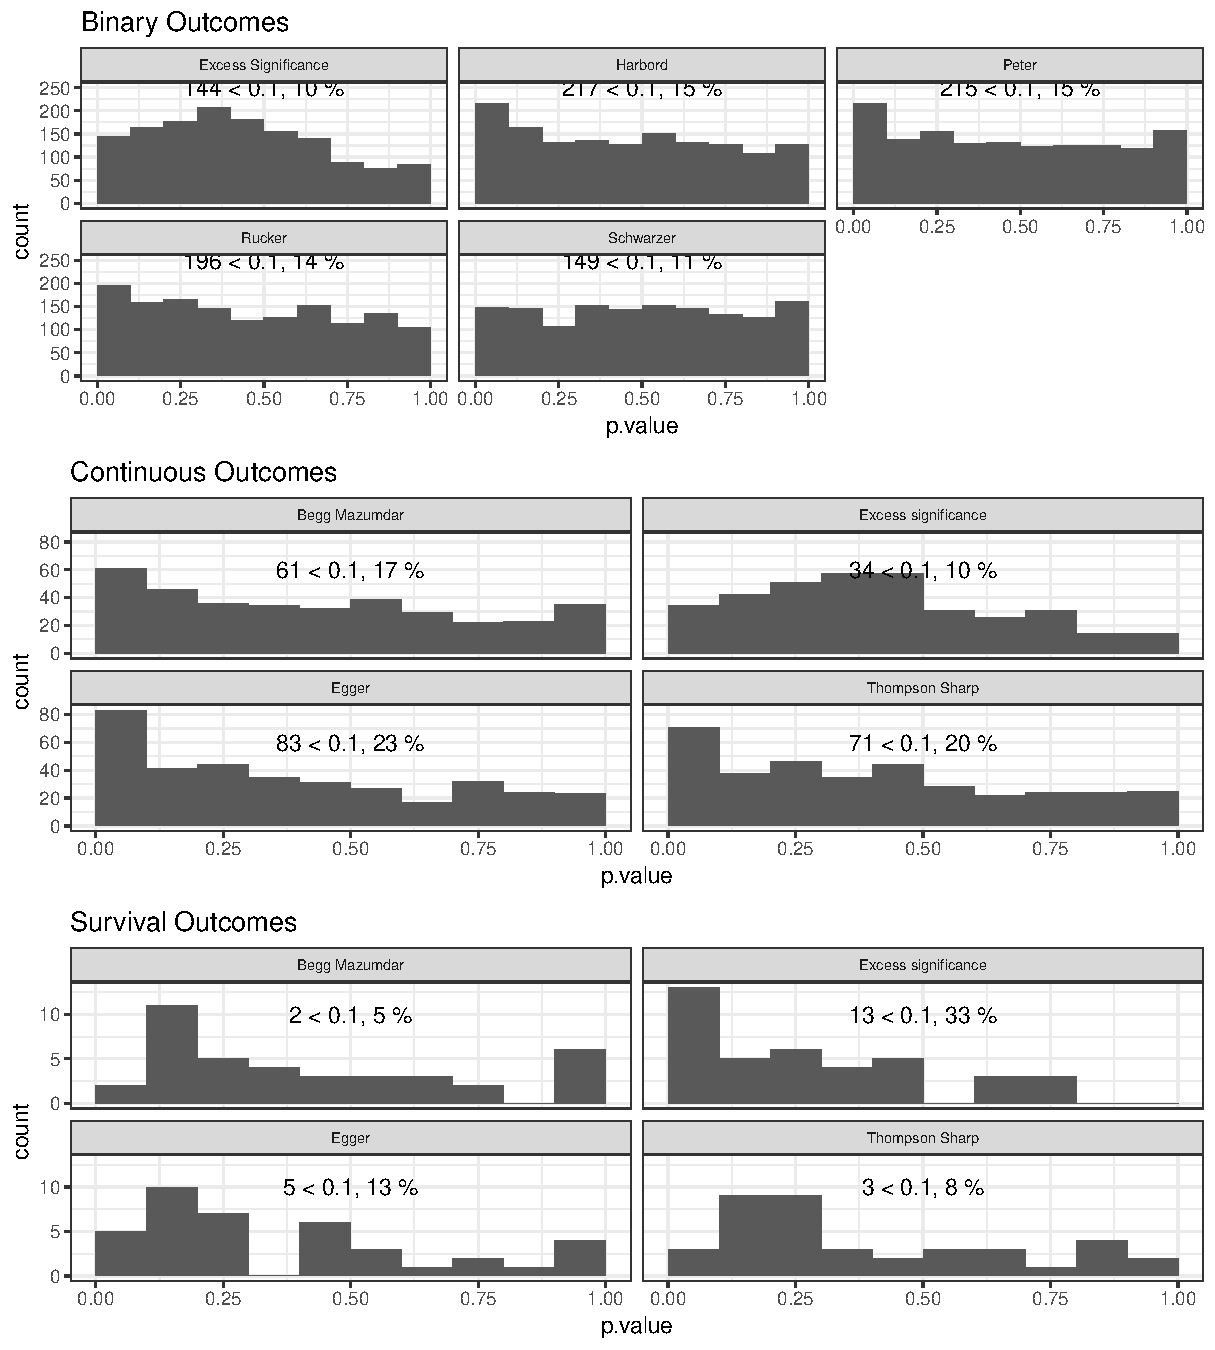
\includegraphics[width=\textwidth-3cm]{figure/ch03_figunnamed-chunk-10-1} 

}



\end{knitrout}
\caption{Histogram of one-sided $p$-values for small study effect in direction of larger effect sizes. The testing method is indicated in the header, bin width is equal to 0.1. The proportion of meta-analyses with signifiant publication bias based on the threshold of 0.1 is displayed inside the figures.}
\label{fig:test}
\end{figure}

%Agreement table -> Chunck 1
The histograms in Figure \ref{fig:test} show that most distributions are clearly skewed to the right, indicating evidence for small study effects. Exceptions from this are the excess significance and Schwarzer's test, and the tests for survival outcomes. There, there is no evidence for publication bias, and the histograms are even skewed to the left (Schwarzer). But note that the sample size of survival outcomes is small ($n$ = 39). \\
There is discrepancy between continuous and binary data test results; the evidence for small study effects in continuous data is clearly larger. Also, we see that the $I^2$ statistic of the proportion of overall between-study heterogeneity is distributed differently for the tests, with results with $I^2 = 0$ being evenly distributed in binary outcomes along the range of $p$-values, while they are more similar to the meta-analyses with larger heterogeneity for continuous outcome.\\
In the literature, the excess significance test is advised to be used in the case of no between study heterogeneity. Since there are no small $p$-values for such meta-analyses, one must conclude that there is no excess significance in the dataset. The obvious correspondence with the heterogeneity statistic however rather suggests that the test is another way to assess between study heterogeneity. Thompson test and R\"ucker's test are designed such that they take into account the between study heterogeneity when assessing small study effects. When no heterogeneity is given, Thompson's test results and Egger's test result should be equal, however, the $I^2$ statistic is computed by a more suitable estimator \citep{paulemandel} of $\tau^2$ as the estimator that Thompson and Sharp's test uses (method of moment estimator of \citet{tau.estimator}, which is more conservative by usually finding larger $\tau^2$). In the part of the histogram with $I^2 > 0$, the two tests are more reliable than the remaining tests, while the opposite is expected from simulations \citep{limitmeta} when $I^2 = 0$.\\

It cannot be seen in Figure \ref{fig:test} if the tests used are finding small study effects for the same meta-analyses. A simple method to check the consistency of test results is to compare scatterplots and empirical Spearman correlations between the test statistics. This is done in Figure \ref{fig:test.agreement}. Here, there is no separation between survival and continuous outcomes. The upper left rectangle is displaying binary outcome results and the lower right continuous and survival outcomes results. Also, the $I^2$ statistic is included. Since no test statistic is used for excess significance tests, it is not shown here

\begin{figure}
\begin{knitrout}
\definecolor{shadecolor}{rgb}{0.98, 0.98, 0.98}\color{fgcolor}

{\centering 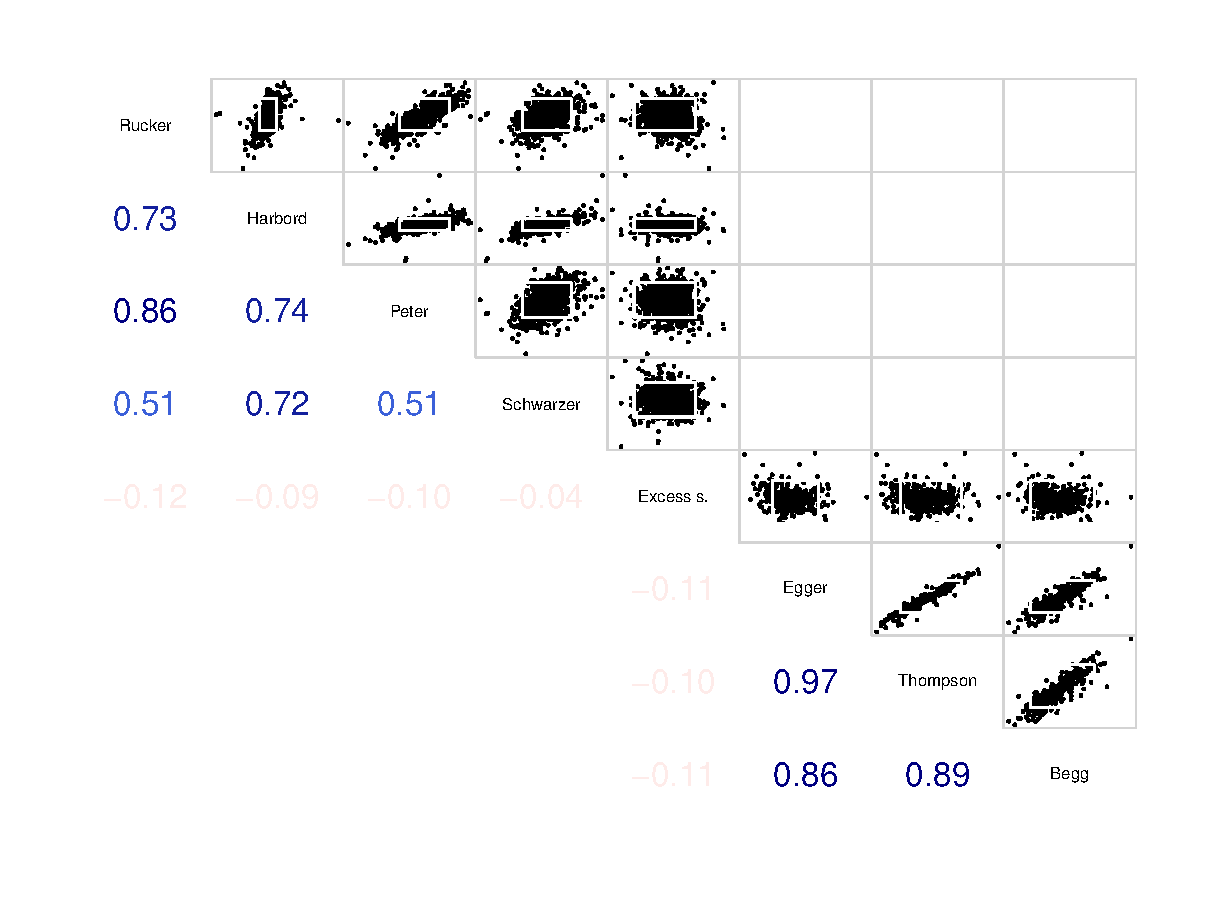
\includegraphics[width=\textwidth-3cm]{figure/ch03_figunnamed-chunk-11-1} 

}



\end{knitrout}
\caption{Pairs-plot for test statistics of small study effect and excess significance. The lower panel gives the Spearman correlations for the different test statistics, and the upper panel displays a scatterplot. The colors indicate magnitude and direction of the correlation coefficients. The rectangle with white borders displays the area within which both tests have absolute value < 1.64 (dots outside are statistically significant by 0.1 $p$-value threshold).}
\label{fig:test.agreement}
\end{figure}

The observed patterns on the scatterplots differ, and some small study effect test statistics do align better than others. Regression based tests as Egger and Thompsons test which are methodically almost identical are closely aligned, which is reflected in large correlation coefficients. Continuous and survival outcome type tests align more closely than binary outcome tests. While correlation coefficients between binary outcome tests vary between each other, Harbord's test statistic has similar correlation coefficients with the other small study effect test statistics.\\
Because scatterplots and correlation coefficients can be misleading, also a Tukey mean-difference or Bland-Altman of transformed $p$-values plot is shown for four scenarios in Figure \ref{fig:mean.diff.test}:
\begin{itemize}
\item For Egger's and Thompson's tests, which is supposedly the most similar test and should show the least deviations and systematic errors
\item For Egger's and excess significance tests
\item For Harbord's and R\"ucker's tests
\item For Harbord's and excess significance tests
\end{itemize}

This can be justified since all tests are supposed to measure the evidence for publication bias. For the plots, the $p$-values of the tests are transformed on the entire continuous scale by a logit transformation $f(x)  = \log\frac{p}{1-p}$). The mean $p$-value (($f$($p$-value no. 1) + $f$($p$-value no. 2))/2) is then displayed against the difference between the $f$($p$-value). If no systematic errors and biases exist between the measurement methods, then 

\begin{itemize}
\item the mean of the differences should be around zero (no systematic error) 
\item the points should scatter independently on the $y$-axis and no general increase or decrease with the mean of the transformed $p$-values should be visible
\end{itemize}

Although this is not formally tested, there are likely systematic errors and bias between excess significance tests, although more so for continuous tests. -- In the appendix, it can be seen that this is reproducible with the remaining small study effect tests (not there yet) -- \\
The confidence intervals from Figure \ref{fig:mean.diff.test} can be used as limits of agreement, which gives, after back-transformation, around 0.9 for Egger's and Thompson's test, and around 0.99 for Harbord's and R\"ucker's tests. This suggests that correspondence between the tests is not very good in general. 

\begin{figure}
\begin{knitrout}
\definecolor{shadecolor}{rgb}{0.98, 0.98, 0.98}\color{fgcolor}

{\centering 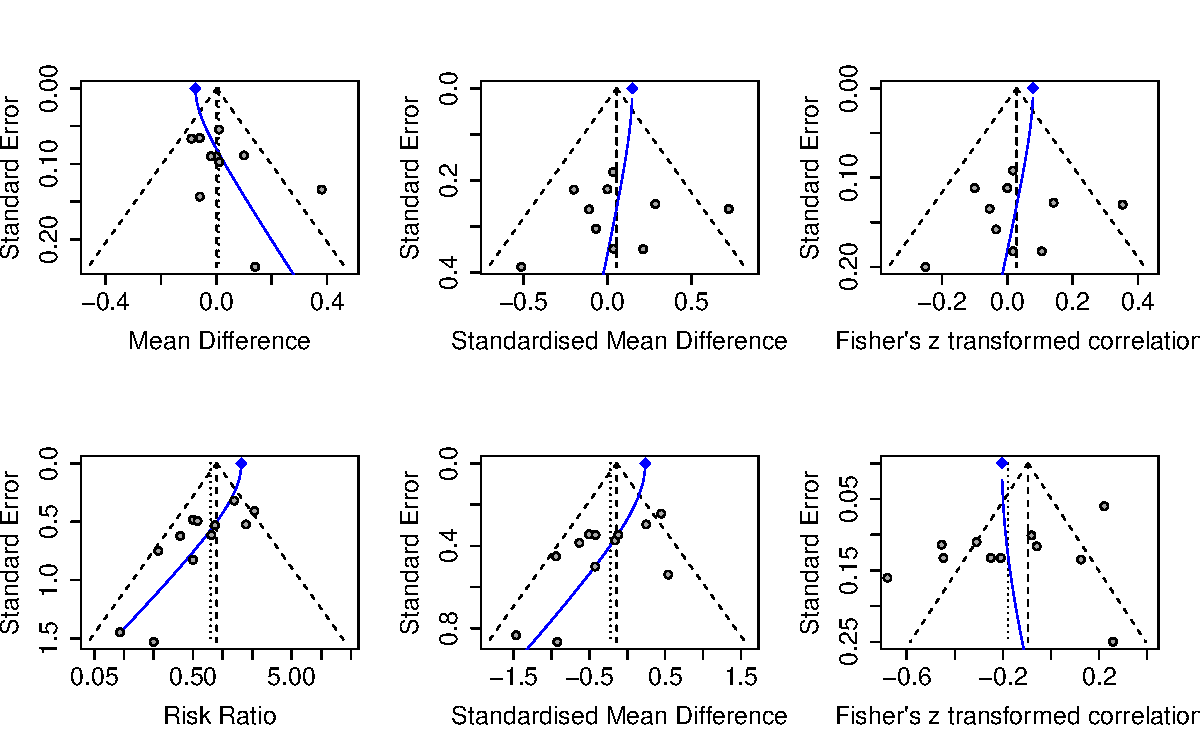
\includegraphics[width=\textwidth-3cm]{figure/ch03_figunnamed-chunk-12-1} 

}



\end{knitrout}
\caption{Mean - difference plots for logit transformed $p$-values. The mean of logit transformed $p$-values is displayed on the $x$-axis and the difference on the $y$-axis. Blue and red lines display the systematic error and the confidence intervals of the systematic error (limits of agreement).}
\label{fig:mean.diff.test}
\end{figure}

The previous results suggest that the results will also differ substantially after applying the common dichotomization of $p$-values. We expect that some proportion of the meta-analysis will only be significant for a certain test, and this is indeed observed in Table \ref{number.sig.tests}. It displays the percentage of meta-analyses with a certain number of significant test results.

% latex table generated in R 3.5.1 by xtable 1.8-3 package
% Fri Jul  5 16:13:26 2019
\begin{table}[ht]
\centering
\begingroup\footnotesize
\begin{tabular}{ccc}
  \hline
Count & Binary Outcomes & Continuous and Survival \\ 
  \hline
0 & 68 \% & 64.3 \% \\ 
  1 & 13.5 \% & 10 \% \\ 
  2 & 7.5 \% & 6.9 \% \\ 
  3 & 5.2 \% & 16.5 \% \\ 
  4 & 4.9 \% & 2.3 \% \\ 
  5 & 0.8 \% & - \\ 
   \hline
\end{tabular}
\endgroup
\caption{Counts Number of significant test results per meta-analysis, separated
       for outcome types. Last entry for continuous and survival outcomes is empty since one test less was 
       applied} 
\label{number.sig.tests}
\end{table}


Here, it is difficult to say if continuous and survival or binary outcome types show better agreement, since more tests are applied in the binary case, and the continuous and survival outcome type tests have in general more positive findings. Very few meta-analyses are significant, irrespective of the test used, but around 67\% of the dataset is not significant, no matter which test is used. \\
When only looking at small study effect tests, 27.3\% of binary outcome tests and 34.4\% of survival and continuous outcome tests had at least one significant result. After applying the Bonferroni correction for multiple testing, this shrinks to 10.5\% for binary and 17.5\% for continuous and survival outcomes. \\
% To compare significant findings for small study effect tests and excess significance tests, we limit ourselves to comparison with Harbord's or Egger's test. mean.min.bin2\% of binary outcome analyses had at least one of the two test $p$-values being significant, and equivalently, mean.min.else2\% for continuous and survival outcomes. The numbers change to mean.min.bin2.b\% for binary outcomes and mean.min.else2.b\% for continuous and survival outcomes after applying the Bonferroni correction. \\
% both.bin\% have significant Harbord's test result and significant excess significance test result  (both.bin.b\% with Bonferroni). Of the continuous outcomes, we have both.else\% with Egger's test and both.else.b\% with Bonferroni correction. 

%%%%%%%%%%%%%%%%%%%%%%%%%%%%%%%%%%%%%%%%%%%%%%%%%%%%%%%%%%%%%%%%%%%%%%%%%%%%%%%%
%%%%%%%%%%%%%%%%%%%%%%%%%%%%%%%%%%%%%%%%%%%%%%%%%%%%%%%%%%%%%%%%%%%%%%%%%%%%%%%%
%%%%%%%%%%%%%%%%%%%%%%%%%%%%%%%%%%%%%%%%%%%%%%%%%%%%%%%%%%%%%%%%%%%%%%%%%%%%%%%%
%%%%%%%%%%%%%%%%%%%%%%%%%%%%%%%%%%%%%%%%%%%%%%%%%%%%%%%%%%%%%%%%%%%%%%%%%%%%%%%%
%%%%%%%%%%%%%%%%%%%%%%%%%%%%%%%%%%%%%%%%%%%%%%%%%%%%%%%%%%%%%%%%%%%%%%%%%%%%%%%%

\section{Small Study Effects Adjustment}


\subsection{Change in Effect Size after Adjustment} \label{sec:change.size}

Since there's evidence for publication bias when applying small study effect and excess significance tests, we apply small study effect adjustment methods to take into account that small studies are likely overestimating the treatment effect. \\
However, we will see that consequences of adjustment can be; 
\begin{itemize}
\item first, the absolute size of the treatment effect can be smaller than the classical meta-analysis treatment effect, which is expected if publication bias
is the cause for the small study effect.
\item secondly, the effect can be larger than before in meta-analysis. In this case, the small study effect must be not due to publication bias for large effects (``true'' publication bias), but due to bias for small effects (``null effect publication bias'' or even ``reversed effect publication bias'', sometimes refer erred to as ``Proteus phenomenon'' \citep{proteus}).
\end{itemize}

This is because, in contrast to the small study effect tests, the applied adjustment method does not pre-specify the direction in which bias is expected. \\
To compare the effects of adjustment between meta-analyses, the outcome measures are transformed to Hedges $g$ (standardized mean differences) and Fisher's $z$-score (see section \ref{sec:transformation.effectsizes} for details). The effect of adjustments can be compared to either random or fixed effects meta-analysis estimates. \\
Figure \ref{fig:adjustment.reg} displays the difference $\delta$ between the observed meta-analysis pooled treatment effect and the regression adjusted treatment effect, $\hat{\theta}_M - \hat{\theta}_\textrm{Adj.}$. The absolute value $|\hat{\theta}_M|$ is taken and the sign of $\hat{\theta}_\textrm{Adj.}$ is adjusted accordingly such that all effects are mirrored to one side. $\delta > 0$ is equivalent to $\hat{\theta}_\textrm{Adj} < \hat{\theta}_M$, a reduction of the original effect size. Additionally, the test statistic of heterogeneity adjusted small study effect tests (R\"ucker's and Thompson's test) is displayed with green color. Test statitics smaller $< 1$ are equivalent to no evidence for small study effect, test statistics between one and two to weak evidence, and above two they indicate evidence for small study effects. Some very large and very small differences have been omitted in the $z$-score and Hedges $g$ histograms; they are shown in Table \ref{missing.differences}. 

\begin{figure}
\begin{knitrout}
\definecolor{shadecolor}{rgb}{0.98, 0.98, 0.98}\color{fgcolor}

{\centering 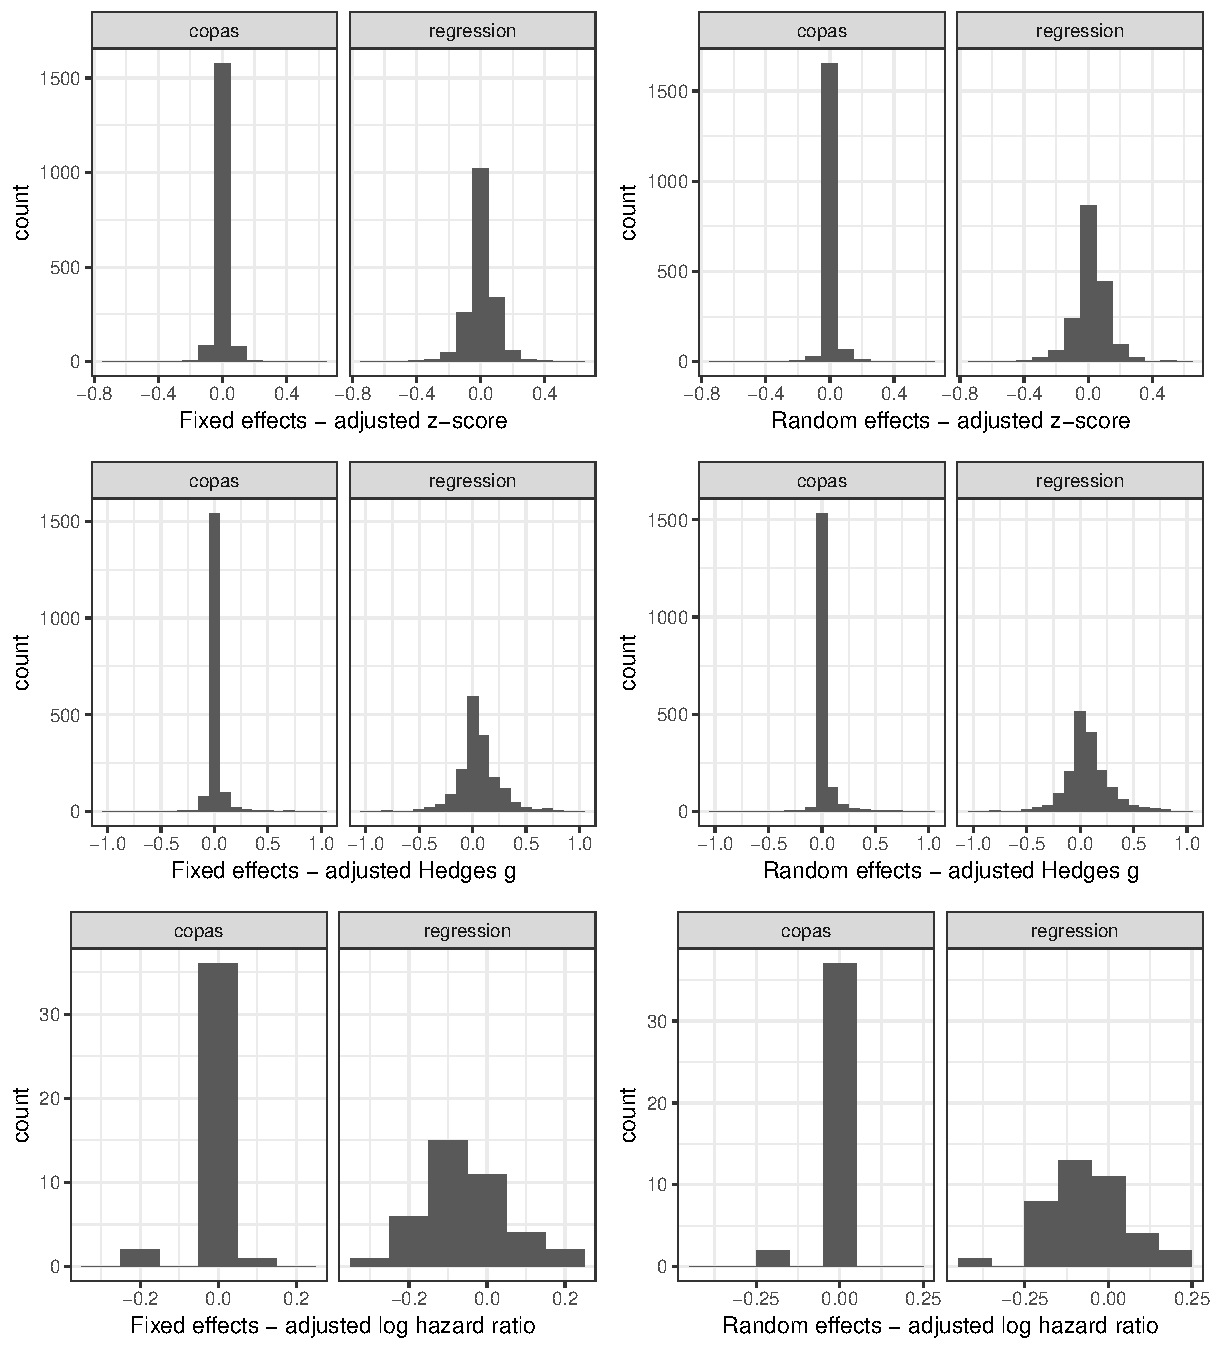
\includegraphics[width=\textwidth-3cm]{figure/ch03_figunnamed-chunk-15-1} 

}



\end{knitrout}
\caption{Histogram of the treatment effect differences between meta-analysis and regression adjusted meta-analysis. Negative differences indicate greater adjusted effect sizes than meta-analysis effect sizes. The bins are centered at zero and binwidth is equal to 0.1. Deeper green color indicates more evidence for small study effects.}
\label{fig:adjustment.reg}
\end{figure}

We see that more treatment effect sizes are negatively adjusted and diminished. Furthermore, we see that large adjustment is not necessarily connected with evidence for small study effects, but there is of course strong coincidence. The cases with no evidence and large adjustment indicate that between-study heterogeneity was not resolved by adjustment for small study effects. Adjustment was larger when random effects meta-analysis effect is used as reference, because there larger weights are given to small studies.\\
Figure \ref{fig:adjustment.copas} shows the same for effect sizes adjusted by Copas; Copas selection model substitutes its estimates with random effect estimates when it finds no evidence for small study effects. Therefore, the effect of adjustment by Copas can be seen when comparing adjusted with random effects estimates. Again, we clearly see that more effect sizes are adjusted downwards. Additionally, there is more coincidence with the small study effect test statistics and adjustment, which is as expected. \\

\begin{figure}
\begin{knitrout}
\definecolor{shadecolor}{rgb}{0.98, 0.98, 0.98}\color{fgcolor}

{\centering 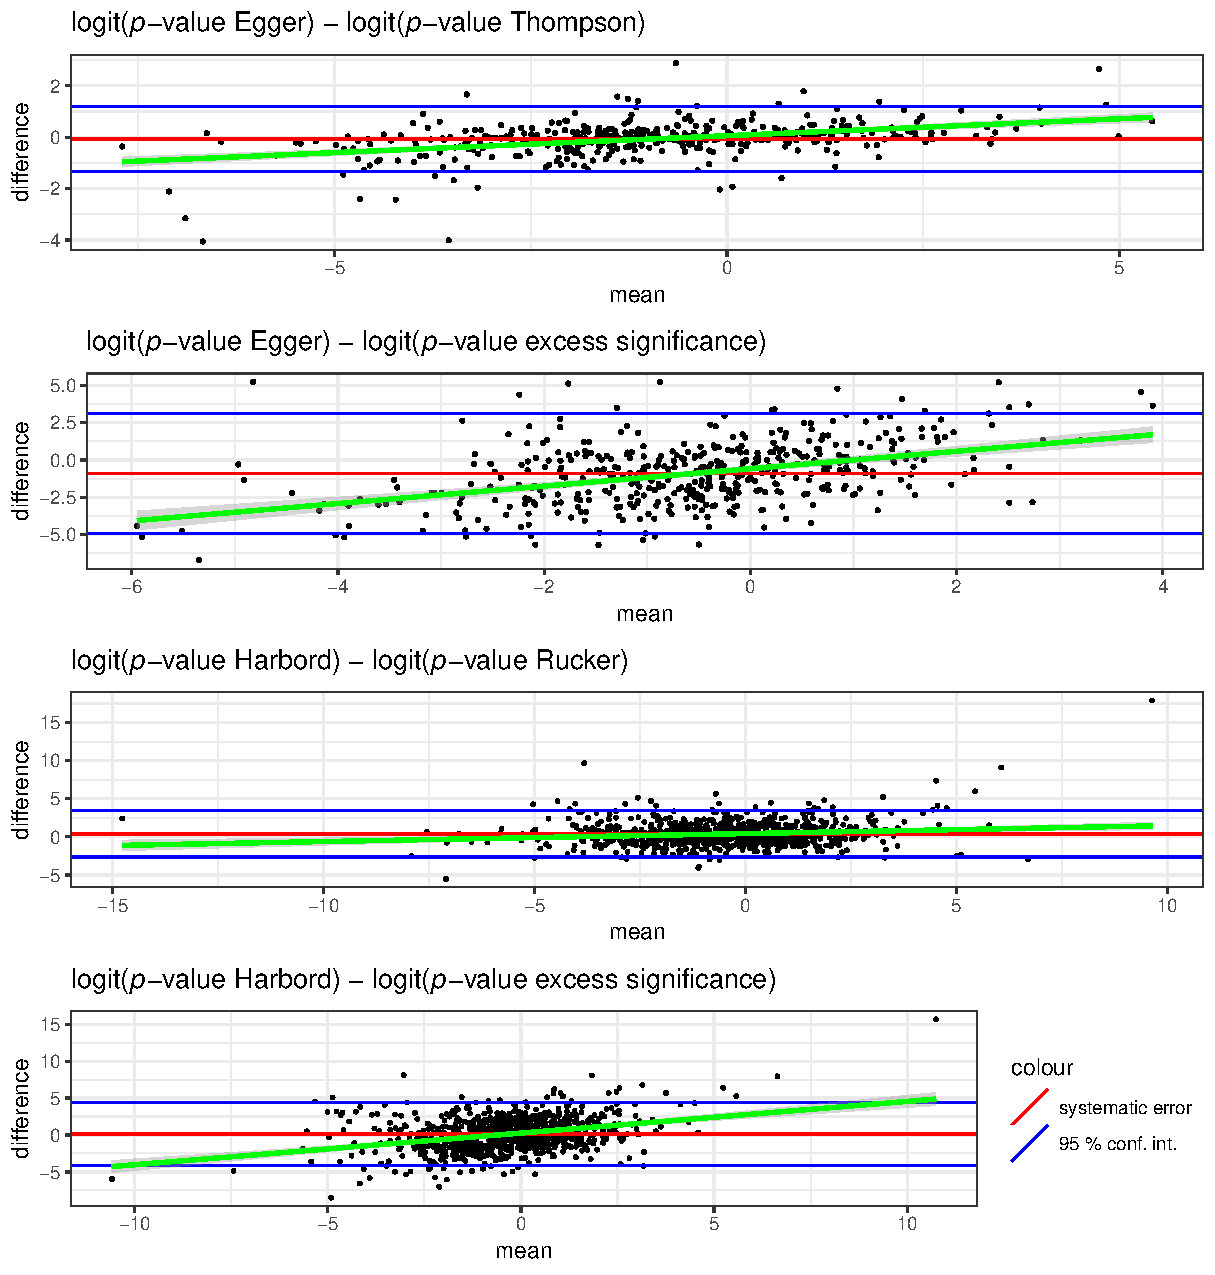
\includegraphics[width=\textwidth-3cm]{figure/ch03_figunnamed-chunk-16-1} 

}



\end{knitrout}
\caption{Histogram of the treatment effect differences between meta-analysis and Copas adjusted meta-analysis. Negative differences indicate greater adjusted effect sizes than meta-analysis effect sizes. The bins are centered at zero and binwidth is equal to 0.1. Deeper green color indicates more evidence for small study effects.}
\label{fig:adjustment.copas}
\end{figure}

Table \ref{adjustment.difference} shows the quantiles and means for the various differences and additional information. When Hedge's $g$ is used as an effect measure, there are (substantially) more reduced effect sizes. The means in Table \ref{adjustment.difference} suggest that the average reduction is small (the means of Copas in the first two rows for $z$-score are caused by one very large value, see Table \ref{missing.differences}). To recall some other findings out of Table \ref{adjustment.difference}: 5\% or 90 cases have their $z$-score reduced by more than 0.15 by regression adjustment (and 5\% or 90 increased by -0.13, fixed effects reference). Also, Hedges $g$ is reduced by 0.39 compared to fixed effects estimates in 5\% or 90 meta-analyses (or increased by 0.24). 

% latex table generated in R 3.5.1 by xtable 1.8-3 package
% Fri Jul  5 16:13:41 2019
\begin{table}[ht]
\centering
\begingroup\scriptsize
\begin{tabular}{lcccccccccr}
  \hline
 & 5\% & 25\% & 50\% & 75\% & 95\% & mean & = 0 (\%) & $>$= 0 (\%) & $>$ 0 (\%) & No adj. est. (\%) \\ 
  \hline
z: Fixed - Copas & -0.05 & -0.01 & -0.00 & 0.01 & 0.05 & -271.73 & 4.76 & 48.67 & 43.91 & 71.54 \\ 
  z: Random - Copas & -0.00 & 0.00 & 0.00 & 0.00 & 0.04 & -263.62 & 71.65 & 89.42 & 17.77 & 71.54 \\ 
  z: Fixed - Regression & -0.13 & -0.03 & 0.01 & 0.05 & 0.14 & 0.01 & 0.00 & 52.44 & 52.44 & 0.17 \\ 
  z: Random - Regression & -0.15 & -0.03 & 0.02 & 0.07 & 0.18 & 0.02 & 0.00 & 57.64 & 57.64 & 0.17 \\ 
  g: Fixed - Copas & -0.05 & -0.01 & 0.00 & 0.01 & 0.09 & 0.02 & 22.76 & 59.14 & 36.38 & 60.96 \\ 
  g: Random - Copas & -0.00 & 0.00 & 0.00 & 0.00 & 0.14 & 0.03 & 63.29 & 87.49 & 24.20 & 60.96 \\ 
  g: Fixed - Regression & -0.23 & -0.04 & 0.03 & 0.13 & 0.38 & 0.05 & 0.00 & 61.96 & 61.96 & 0.00 \\ 
  g: Random - Regression & -0.24 & -0.03 & 0.05 & 0.16 & 0.42 & 0.06 & 0.00 & 64.06 & 64.06 & 0.00 \\ 
  Log h.r.: Fixed - Copas & -0.02 & 0.00 & 0.00 & 0.00 & 0.02 & -0.00 & 46.15 & 35.90 & 82.05 & 56.41 \\ 
  Log h.r.: Random - Copas & -0.02 & 0.00 & 0.00 & 0.00 & 0.00 & -0.01 & 61.54 & 17.95 & 79.49 & 56.41 \\ 
  Log h.r.: Fixed - Regression & -0.20 & -0.13 & -0.06 & 0.02 & 0.14 & -0.05 & 0.00 & 33.33 & 33.33 & 0.00 \\ 
  Log h.r.: Random - Regression & -0.22 & -0.14 & -0.07 & 0.03 & 0.14 & -0.06 & 0.00 & 33.33 & 33.33 & 0.00 \\ 
   \hline
\end{tabular}
\endgroup
\caption{Quantiles and Means of the differences between meta-analysis pooled treatment effects and small study adjusted treatment effects. The column with the names ``> 0'' give the percentages of estimates larger than zero or larger or equal zero. The column ``No adj. est.'' gives the percentage of missing estimates due to non-significant publication bias test (for Copas) and computational errors. The row names indicate which outcome measure, meta-analysis method and adjustment method is used. Abbreviations are used for z-score (= z) and Hedges g (= g).} 
\label{adjustment.difference}
\end{table}



\subsection{Change in Evidence for Treatment Effects} \label{sec:change.evidence}
Adjustment for small study effects in meta-analysis will not only provide new effect sizes, but also standard errors thereof. Thus, also the evidence for efficacy of a treatment can be obtained, which is usually summarized in a suitable test statistic or $p$-value. It is of interest if and how the evidence for treatment effects changes if adjusted for publication bias.\\
The Wald test statistics $p$-value for fixed and random effects meta-analyses and Copas and regression adjusted treatment effects have been calculated. They are shown in Figure \ref{fig:adjustment.stat} for meta-analysis based on $z$-score, Hedges $g$ and log hazard ratios. \\
It can be seen that evidence for a treatment effect decreases after adjusting for publication bias. It does so more for Hedge's $g$ compared to $z$-scores, and for regression adjustment compared to Copas selection model. 
%Also, the evidence decreases for random effects meta-analyses compared to fixed effects meta-analyses. 
In the case of log-hazard ratio adjustment, the adjustment has only negligible impact on the $p$-values. \\
Also, Copas selection method has a very small impact on the evidence compared to random effects meta-analysis, at least using $z$-scores (again, we should rely on comparisons to random effects meta-analysis to evaluate Copas method). \\ 
% Interestingly, in contrast to the small study effect tests, there seems to be no large difference between adjusted continuous and binary meta-analysis test statistics --appendix--
%Figures \ref{fig:adjustment.stat.z} for the adjusted $z$-scores, \ref{fig:adjustment.stat.smd} for the adjusted Hedges $g$ and Cohen's d and \ref{fig:adjustment.stat.log.hazard.ratio} for the adjusted log hazard ratios.

\begin{figure}
\begin{knitrout}
\definecolor{shadecolor}{rgb}{0.98, 0.98, 0.98}\color{fgcolor}

{\centering 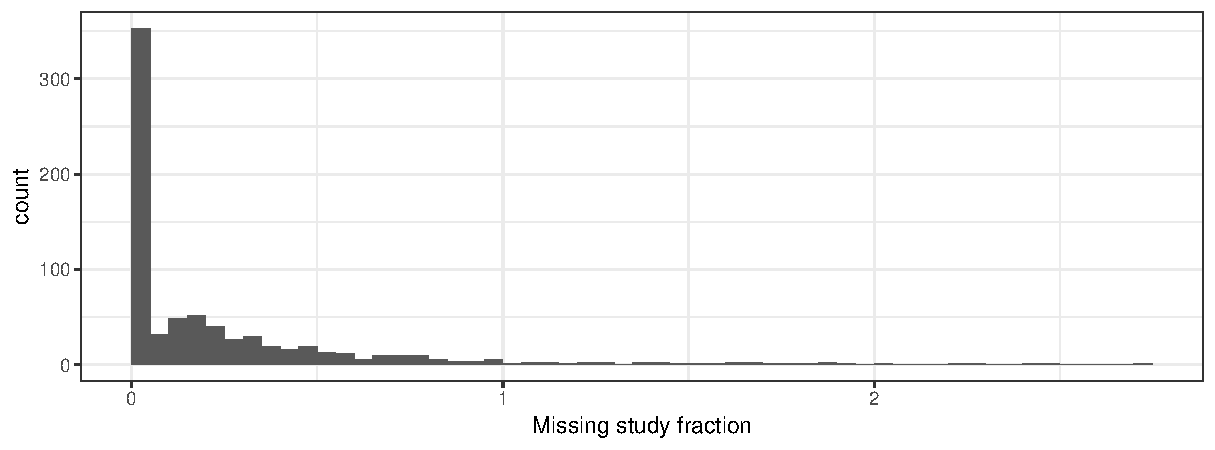
\includegraphics[width=\textwidth-3cm]{figure/ch03_figunnamed-chunk-18-1} 

}



\end{knitrout}
\caption{Histogram of the Wald test-statistic $p$-value of meta-analysis and adjusted pooled treatment effect, based on different treatment effect measures. The method is indicated in the header, bin width is set to 0.05. The significant proportion based on the threshold of 0.05 is displayed inside the figures.}
\label{fig:adjustment.stat}
\end{figure}

The Copas selection model also gives an estimate of the number of missing studies. It finds that 0 are missing, which corresponds to 0\% from all \ensuremath{2.8945\times 10^{4}} analysed studies. Figure \ref{fig:copas.missing} shows a histogram of the overall fraction of missing studies. Note that we have excluded 0 out of 1806, for which no Copas selection model estimate, but a random effects estimate was retained because the algorithm initially found no evidence for small study effects.

\begin{figure}
\begin{knitrout}
\definecolor{shadecolor}{rgb}{0.98, 0.98, 0.98}\color{fgcolor}

{\centering 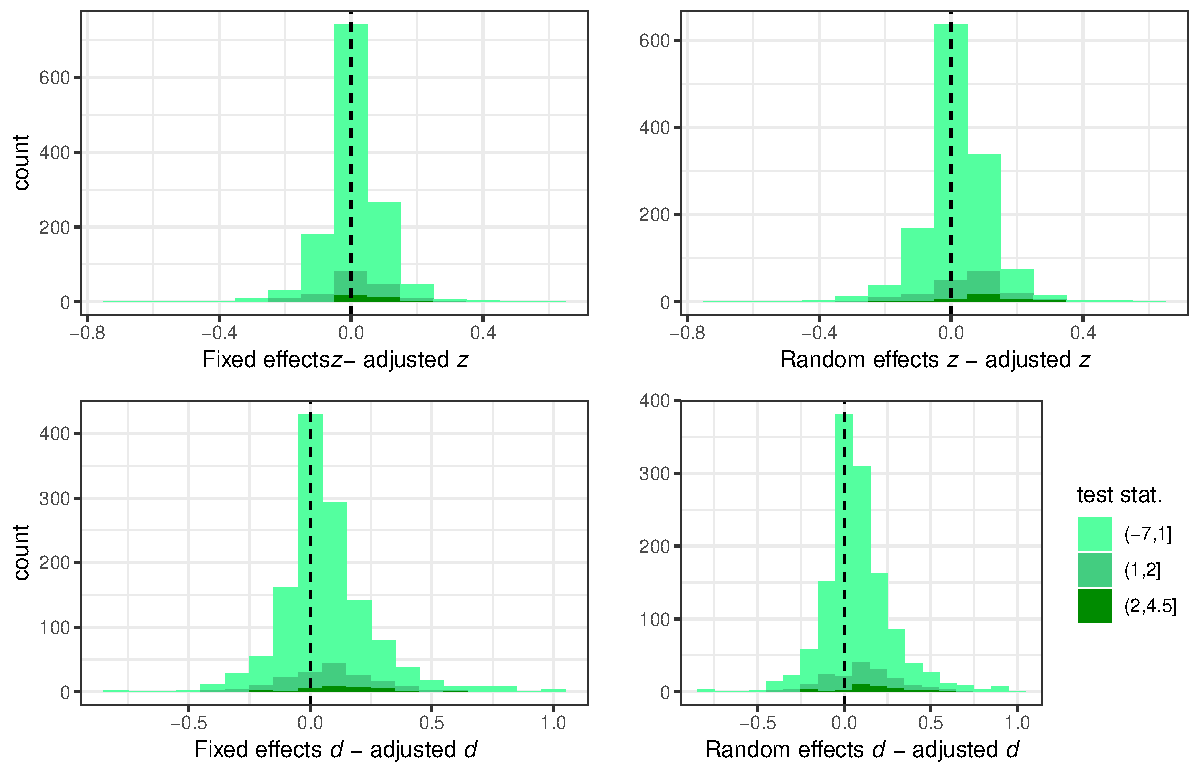
\includegraphics[width=\textwidth-3cm]{figure/ch03_figunnamed-chunk-19-1} 

}



\end{knitrout}
\caption{Histogram of the fraction of missing studies from the total number of studies in a meta-analyses (only data shown where Copas estimate was obtained, thus \\$n =$ 0)}
\label{fig:copas.missing}
\end{figure}

We can see that in some occasions, the method finds more than half of all studies are missing. In most occasions, the estimate of missing studies is zero, as can be seen in Table \ref{copas.missing}. The discrepancy between mean and median may indicate that the estimate of 0\% missing studies depends somewhat on these extreme cases. As can be written of from Table \ref{copas.missing}, 5\%, \ie 0 meta-analyses have 17.6 or more studies missing: in fact, these 5\% most extreme make up for 0, more than 30\% of missing studies.

% latex table generated in R 3.5.1 by xtable 1.8-3 package
% Fri Jul  5 16:13:42 2019
\begin{table}[ht]
\centering
\begingroup\footnotesize
\begin{tabular}{lrrrrrrr}
  \hline
 & = 0 & 5\% & 25\% & 50\% & 75\% & 95\% & mean \\ 
  \hline
Missing fraction & 323 & 0 & 0 & 0.1 & 0.3 & 1.0 & 0.2 \\ 
  Missing study number & 323 & 0 & 0 & 1.4 & 5.2 & 17.9 & 4.2 \\ 
   \hline
\end{tabular}
\endgroup
\caption{Fraction of missing studies and estimates of missing studies with their zero counts (``= 0''), quantiles and means.} 
\label{copas.missing}
\end{table}






% latex table generated in R 3.5.1 by xtable 1.8-3 package
% Fri Jul  5 16:13:42 2019
\begin{table}[ht]
\centering
\begingroup\tiny
\begin{tabular}{lcccrrrrrrrr}
  \hline
meta.id & file.nr & comparison.nr & subgroup.nr & z fixed & z random & z Copas & z regression & g fixed & g random & g Copas & g regression \\ 
  \hline
2009 & 2009 & 1 & 1 & 0.31 & 0.36 & 0.31 & 0.43 & 0.70 & 0.70 & 0.70 & 2.48 \\ 
  2068 & 2068 & 2 & 0 & 0.29 & 0.35 & 0.29 & 0.42 & 0.68 & 0.68 & 0.68 & 2.57 \\ 
  52528 & 52528 & 1 & 0 & -0.75 & -0.69 & -0.50 & -0.26 & -1.19 & -1.53 & 0.18 & -0.52 \\ 
  60546 & 60546 & 1 & 1 & 0.17 & 0.24 & 0.17 & 0.34 & 0.53 & 0.53 & 0.53 & 1.65 \\ 
  70389 & 70389 & 1 & 1 & -0.08 & -0.07 & 15.62 & -0.04 & -0.13 & -0.13 & -0.13 & -0.05 \\ 
  73769 & 73769 & 3 & 1 & -0.09 & 0.00 & 7148.96 & 0.02 & -0.01 & -0.12 & 0.01 & 0.04 \\ 
  79113 & 79113 & 2 & 0 & -0.38 & -0.38 & -0.38 & -0.48 & -0.93 & -0.93 & -2.00 & -3.47 \\ 
  90138 & 90138 & 3 & 0 & 0.30 & 0.80 & 0.30 & 0.53 & 0.72 & 0.71 & 0.71 & 2.16 \\ 
  97356 & 97356 & 2 & 0 & -0.06 & -0.33 & -0.06 & -0.11 & -0.42 & -0.35 & -1.58 & -1.82 \\ 
  98030 & 98030 & 1 & 0 & -0.09 & -0.07 & -0.09 & -0.04 & -0.41 & -0.41 & -1.50 & -2.79 \\ 
  101436 & 101436 & 1 & 5 & 0.54 & 0.62 & 0.80 & 0.90 & 1.21 & 1.21 & 1.21 & 2.74 \\ 
  118121 & 118121 & 4 & 1 & 0.25 & 0.23 & 47.73 & -0.03 & 0.44 & 0.44 & 0.44 & 0.14 \\ 
  119537 & 119537 & 3 & 0 & 0.07 & 0.15 & 0.07 & 0.29 & 0.50 & 0.50 & 1.43 & 1.81 \\ 
  119818 & 119818 & 3 & 3 & -0.25 & -0.25 & -0.20 & -0.04 & -0.50 & -0.54 & 28.44 & -0.03 \\ 
  146301 & 146301 & 1 & 0 & 0.14 & 0.26 & 472149.03 & 0.28 & 0.56 & 0.37 & 0.60 & 0.52 \\ 
   \hline
\end{tabular}
\endgroup
\caption{Missing meta-analysis pooled treatment effect and adjusted treatment effects. Abbreviations are used for z-score (= z) and Hedges g (= g).} 
\label{missing.differences}
\end{table}




\subsection{Comparison of adjustment methods}
Regression adjusted estimates are compared to the estimates of Copas selection model if these are not equal to random effects meta-analysis. A Tukey mean difference plot can serve to reveal systematic differences and biases between the two measurement methods. We will compare estimates based on all three outcome measures, i.e. original measure, $z$-score and Hedges $g$ in Figure \ref{fig:adjustment.mean.diff}. Note that the 39 survival outcome data is not included when using $z$-score and Hedges $g$.

\begin{figure}
\begin{knitrout}
\definecolor{shadecolor}{rgb}{0.98, 0.98, 0.98}\color{fgcolor}

{\centering 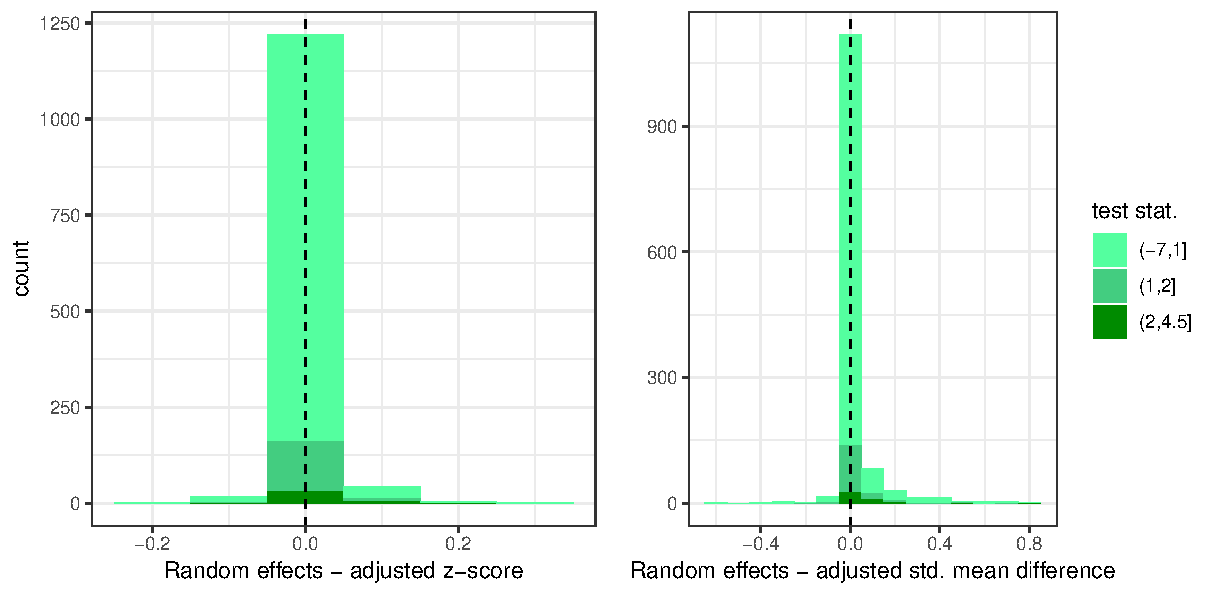
\includegraphics[width=\textwidth-3cm]{figure/ch03_figunnamed-chunk-22-1} 

}



\end{knitrout}
\caption{Mean - difference plots for publication bias adjustment methods. The mean of the adjusted treatment effects is displayed on the $x$-axis and the difference on the $y$-axis. Blue and red lines display the systematic error and the confidence intervals of the systematic error (limits of agreement). Two values have been omitted in the middle plot for Hedges $g$ and one for $z$-score (see Table \ref{missing.differences}).}
\label{fig:adjustment.mean.diff}
\end{figure}

No formal tests are provided, but the at least there seems to be no clear bias or systematic error. The limits of agreement in Figure \ref{fig:adjustment.mean.diff} are large. We conclude thus that the impact of regression adjustment on the effect sizes is in general not substantially larger than the impact of Copas selection model in the subset of data where the estimate of the Copas selection model is not equal to a random effects estimate. There is however a small difference, with regression estimates to have a little bit a larger absolute value. There might be some bias between adjusted $z$-scores, where regression estimates seem to be somewhat smaller when the mean is a little above zero, and somewhat larger when the mean is a little below zero. \\


%%%%%%%%%%%%%%%%%%%%%%%%%%%%%%%%%%%%%%%%%%%%%%%%%%%%%%%%%%%%%%%%%%%%%%

%<<'child-chapter05', child='chapter05.Rnw'>>=
%@

%%%%%%%%%%%%%%%%%%%%%%%%%%%%%%%%%%%%%%%%%%%%%%%%%%%%%%%%%%%%%%%%%%%%%%

\appendix

% LaTeX file for Chapter 01



\chapter{Appendix}

Maybe some R code here, probably a \rr{sessionInfo()}




\cleardoublepage
\phantomsection
\addtocontents{toc}{\protect \vspace*{10mm}}
\addcontentsline{toc}{chapter}{\bfseries Bibliography}


\bibliographystyle{mywiley} 
\bibliography{biblio}

\cleardoublepage

\end{document}

